\documentclass[fleqn, final]{../styles/unmphythesis}
\usepackage{../styles/qxd}
\renewcommand{\thechapter}{2}
%\newcommand{\thechapter}{1}

\makeindex
\begin{document}

%<*waveguideinterface>

\chapter{Atom-waveguide interfaces}
\section{Introduction}
In this chapter, we look at the case that only one atom is trapped nearby a waveguide. As will be discussed later, in the dispersive regime, the interaction from many atoms can be treated as a sum of the interactions from all individual atoms. To be specific, for this chapter, we consider the following scenario: a laser beam propagates through a waveguide along $ z $ direction; an alkali atom (cesium, for example) is trapped at $ \mathbf{r}_{\rm atom} =\mathbf{r}'$ in the evanescent field of the waveguide~\footnote{We will use the prime ($ ' $) notation to indicate the position of a photon emitter.} and responds to the guided optical field dispersively. In the dynamics, the atom can be treated as an optical dipole that adiabatically eliminates from an excited state to the ground state as an effective two-level system. The light, on the other hand, experiences dispersive phase shift and usually negligible intensity attenuation afterwards. Effectively, the presence of the atom outside of the waveguide changes the index of refraction\index{index of refraction} of the waveguide. 
The dispersive light shift applies when the saturation parameter is small,
\begin{align}
s=\frac{\Omega^2/4}{\Delta^2+\Gamma^2/4}\ll 1,
\end{align}
where $ \Omega $ is the Rabi frequency, $ \Gamma $ is the spontaneous emission rate of the atom, and $ \Delta=\omega_0-\omega_{eg} $ is the probe detuning from the atomic resonance frequency $ \omega_{eg} $ as a two-level system with the probe's frequency set to be $ \omega_0 $. 

\begin{figure}
\centering\makebox[\textwidth]{
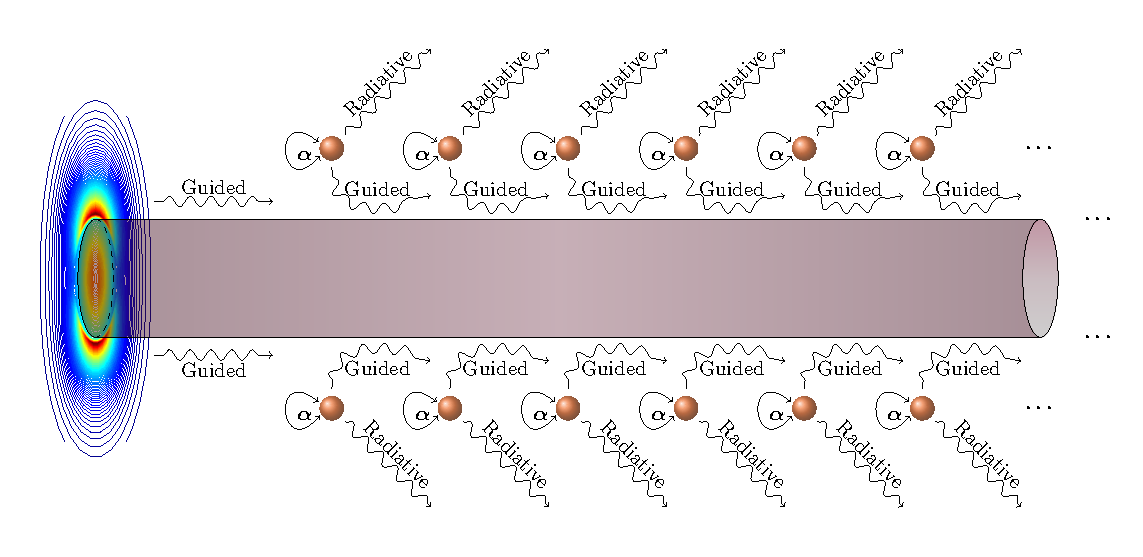
\includegraphics[width=0.85\textwidth]{../media/Figs/NanofiberTrappedAtoms}}
\caption[Guided and radiative photon emissions from atoms trapped next to a nanophotonic waveguide.]{Guided and radiative photon emissions from atoms trapped next to a nanophotonic waveguide. In the dispersive regime and when the atoms are placed a few hundred nm away from each other, the effect of the unguided radiation from the atoms can be ignored, and the photon scatterings among atoms are also negligible. For a quantum-measurement--targeted research, we mainly care about how the atomic emissions got modified by the waveguide interface and coupled to the guided modes to be detected at the measurement apparatus. Color contour on the left-hand part is an illustration of one guided mode intensity distribution of an optical nanofiber, which leaks into the free space to interact with atoms and propagates through the fiber. }\label{fig:trappedatomradiation}
\end{figure}

In this chapter, we will first outline the basic concept of the polarization state of light and introduce the experimental setup in characterizing the dispersive light shift interaction, which is called \emph{polarization spectroscopy}\index{polarization spectroscopy}.
The theme of this dissertation is set based on the atom-light interactions which includes two aspects: one is how the light respond to the presence of the atoms, and the other is how the atoms' properties are modified by the light. For the light response aspect, we will derive a general theory in the language of Green's function to formulate the atom-light interaction mainly from the semi-classical perspective where the light is treated as a continuous wave while the atom has discrete level structures. 
In simulations, we will show the radiation modes of the waveguides do not propagate too far from atoms and can be ignored for the light response detected at the measurement apparatus (see Fig.~\ref{fig:trappedatomradiation}).
For the atoms' response, we will extend the definition of polarizability of atoms from a classical oscillator picture to the multiple-level quantum representation, and then introduce the Purcell effect and derive the modified spontaneous decay rates of atoms in presence of a waveguide using the Green's function language. 
We will show the modifications of spontaneous emissions when atoms are placed at certain distance can be ignored.
At the end of this chapter, we will conclude with some geometric explanations on the unique features and advantages of using a nanophotonic waveguide interface to implement atom-light coupling over the free-space interface commonly employed in previous experiments.

\section{Polarization spectroscopy and dispersive light shift measures}
\subsection{Polarization states of light}
In free space, light is a transverse field. The polarization state of light\index{polarization} can be fully described by the amplitudes and relative phase of two orthogonal electric field components, $ \mathbf{E}_x $ and $ \mathbf{E}_y $. That is one can write the electric field of a propagating mono-chromatic light field as 
\begin{equation} \label{eq:freeEfield}
\mathbf{E}(\br,t)=\mathbf{E}_x(\br,t)+\mathbf{E}_y(\br,t)
\end{equation} 
with the two orthogonal components~\cite{Jackson1975}
\begin{align}
\mathbf{E}_x(\br,t) &= \mathcal{E}_{x}\mathbf{e}_x e^{i(k_0z-\omega_0 t)}\\
\mathbf{E}_y(\br,t) &= \mathcal{E}_{y}\mathbf{e}_y e^{i(k_0z-\omega_0 t)},
\end{align}
where $ \mathcal{E}_{0x} $ and $ \mathcal{E}_{0y} $ are the complex amplitudes, and $ \mathbf{e}_x $ and $ \mathbf{e}_y $ are the respective direction vectors along the $ x $- and $ y $-axes in the transverse plane perpendicular to the propagation direction along the $ z $ axis. 

A light is said to be \emph{linearly polarized}\index{polarization!linear polarization} if $\mathcal{E}_{x}$ and $ \mathcal{E}_{y} $ have the same phase. The polarization direction is set by the polarization angle $ \theta=\arctan(\mathcal{E}_{y}/\mathcal{E}_{x}) $ from $ \mathbf{e}_x $ direction.
The polarization magnitude is defined to be $ E=\sqrt{\mathcal{E}_{x}^2+\mathcal{E}_{y}^2} $.

A light is said to be \emph{circularly polarized}\index{polarization!circular polarization} if $\mathcal{E}_{x}$ and $ \mathcal{E}_{y} $ have the same magnitude but differ in phase by $ 90^\circ $. The wave can then be described by 
\begin{align}\label{eq:circularlightfield}
\mathbf{E}=E_0(\mathbf{e}_x \pm i\mathbf{e}_y)e^{i(k_0z-\omega_0 t)}
\end{align}
with $ E_0 $ the common real amplitude. Taking any point $ \br_0=(x_0,y_0,z_0) $ in space, the combined polarization vector $ \mathbf{e}_l(z_0)=(\mathbf{e}_x \pm i\mathbf{e}_y)e^{i(k_0z_0-\omega_0 t)} $ sweeps around in a circle at an angular frequency $ \omega_0 $. To see this, we can find the actual electric field components to be observed by taking the real part of the Eq.~\eqref{eq:circularlightfield} to give
\begin{subequations}\label{eq:circularpolinxybasis}
\begin{align}
E_x (\br,t) &= E_0\cos(k_0z-\omega_0 t)\\
E_y (\br,t)&= \mp E_0\sin(k_0z-\omega_0 t).
\end{align}
\end{subequations}
The upper sign corresponding to the $ (\mathbf{e}_x + i\mathbf{e}_y) $ basis indicates the rotation is clockwise if the observer is hit by the propagating light. The light in this case is said to be \emph{left-circularly polarized}\index{polarization!circular polarization!left-circular polarization} in optics, and has a \emph{positive helicity}\index{polarization!positive helicity} in modern physics. Correspondingly, the lower sign, $ (\mathbf{e}_x - i\mathbf{e}_y) $, indicates the light is counterclockwise rotating at a fixed point and is \emph{right-circularly polarized}\index{polarization!circular polarization!right-circular polarization}, and \emph{negative helicity}\index{polarization!negative helicity}. Therefore, one can define the circular polarization basis by the complex orthogonal unit vectors
\begin{align}
\mathbf{e}_{\pm}=\frac{1}{\sqrt{2}}(\mathbf{e}_x \pm i\mathbf{e}_y)
\end{align}
with properties
\begin{align}
\mathbf{e}_q\cdot \mathbf{e}_{q'}^* &=\delta_{q,q'}\\
\mathbf{e}_q^* &=\mathbf{e}_{-q}
\end{align}
where the field has been decomposed into the $ q=\pm $ components by 
\begin{align} 
\mathbf{E}&=\sum_q \mathcal{E}_q\mathbf{e}_q=\mathcal{E}_+ \mathbf{e}_+ +\mathcal{E}_-\mathbf{e}_-\\
&=\mathcal{E}_L\mathbf{e}_++\mathcal{E}_R\mathbf{e}_- 
\end{align} 
with $ \mathcal{E}_q=\mathbf{e}_q^*\cdot \mathbf{E} $, and the left- and right-circular polarization amplitudes $ \mathcal{E}_L=\mathcal{E}_+ $ and $ \mathcal{E}_R=\mathcal{E}_- $, respectively. 
Note that the definition of \emph{left} and \emph{right} rotations in modern physics, including quantum mechanics, is different from that in traditional optics. In order to match the classical definitions of basic concepts with the quantum mechanical derivation in Chapter~\ref{chap:quantumdynamicsrepresentation}, we will primarily stick to the definition of \emph{helicity} in this chapter. 

The Cartesian basis of the polarization measurement is usually called as the linear polarization basis (see Eq.~\eqref{eq:circularlightfield} for the circular polarization case). We can also use $ H $ (horizontal) and $ V $ (vertical) to label the $ x $ and $ y $ components of the field.
Alternatively, if the actual field is detected in the circular polarization basis, only one non-zero amplitude may be detected proportional to the circular polarization component 
\begin{align}
E_\pm(\br_0,t) &= \re\left[\mathbf{e}_\pm^* \cdot \mathbf{E}\right] = \re\left[\mathcal{E}_\pm \right].
\end{align}
I will label the polarization bases of positive and negative helicities with $ + $ and $- $ subscripts, respectively, in this dissertation. The choice of basis of polarization measurement can be operated by using beam splitters and proper wave planes in real experiments~\cite{Born1999Principles}.

If $\mathcal{E}_{x}$ and $ \mathcal{E}_{y} $ have different phases, the light is \emph{elliptically polarized}\index{polarization!elliptical polarization} in general. Represented in the circular polarization basis, the wave can be given by
\begin{align}
\mathbf{E}=(\mathcal{E}_+\mathbf{e}_+ + \mathcal{E}_-\mathbf{e}_-)e^{i(k_0z-\omega_0 t)},
\end{align}
where $ \mathcal{E}_\pm $ are complex amplitudes, and $ \mathrm{angle}\left[\mathcal{E}_+\right]$ may not equal to $\mathrm{angle}\left[\mathcal{E}_-\right] $.
When $ \mathcal{E}_+ $ and $ \mathcal{E}_- $ have different magnitudes yet the same phase, the light is elliptically polarized with the $ \mathbf{E} $ vector traced as an ellipse defined by the principle axes pointing along $ \mathbf{e}_x $ and $ \mathbf{e}_y $ directions~\cite{Jackson1975}. The semimajor and semiminor axes of the ellipse have a ratio of $ |(1+r)/(1-r)| $, where $ r=\mathcal{E}_+/\mathcal{E}_- $. 
When the two complex amplitudes in the circular polarization basis has a phase difference, $ \phi $, or $ \mathcal{E}_+/\mathcal{E}_-=re^{i\phi} $, then the traced ellipse of the $ \mathcal{E} $ vector has its principal axes rotated by an angle $ \phi/2 $ from the $ \mathbf{e}_x $ and $ \mathbf{e}_y $ axes. 
The real parameter $ r $ is the ellipticity\index{polarization!ellipticity} of the ellipse of the $ \mathbf{E} $ vector trace. For $ r=\pm 1 $, we recover the linear polarization case. 

\subsection{Stokes vectors and polarization measurement}

To help visualize the polarization state of the light, we rewrite the field amplitudes\footnote{In the terminology of modern physics, they are also the components of Jones vectors defining a polarized light~\cite{Born1999Principles}.} in the linear and circular polarization bases by
\begin{align}
\mathcal{E}_x &= E_x e^{i\delta_x},\quad & \mathcal{E}_y &= E_y e^{i\delta_y},\\
\mathcal{E}_+ &= E_+ e^{i\delta_+},\quad & \mathcal{E}_- &= E_- e^{i\delta_-},
\end{align} 
where $ E_{x/y} $, $ E_\pm  $, $ \delta_{x/y} $ and $ \delta_\pm $ are all real parameters. Traditionally, the Stokes vector $ \mathbf{S}=(S_0,S_1,S_2,S_3) $ is usually employed in literature to uniquely project the polarization state of the light onto the famous \Poincare sphere\cite{Born1999Principles} (see Fig.\ref{fig:Poincaresphere}). In terms of the linear polarization basis $ (\mathbf{e}_x,\mathbf{e}_y) $, the Stokes vector components are~\cite{Born1999Principles}
\begin{subequations}\label{eq:S_xybasis}
\begin{align}
S_0 &= |\mathbf{e}_x\cdot \mathbf{E}|^2+|\mathbf{e}_y\cdot \mathbf{E}|^2 =E_x^2+E_y^2\\
S_1 &= |\mathbf{e}_x\cdot \mathbf{E}|^2-|\mathbf{e}_y\cdot \mathbf{E}|^2 =E_x^2-E_y^2\\
S_2 &= 2\re\left[ (\mathbf{e}_x\cdot \mathbf{E})^*(\mathbf{e}_y\cdot \mathbf{E})\right] =2E_xE_y\cos(\delta_y-\delta_x)\label{eq:S2_xybasis}\\
S_3 &= 2\im\left[ (\mathbf{e}_x\cdot \mathbf{E})^*(\mathbf{e}_y\cdot \mathbf{E})\right] =2E_xE_y\sin(\delta_y-\delta_x)
\end{align}
\end{subequations}

\begin{figure}[ht] % Poincare sphere.
   \centering\makebox[\textwidth]{
   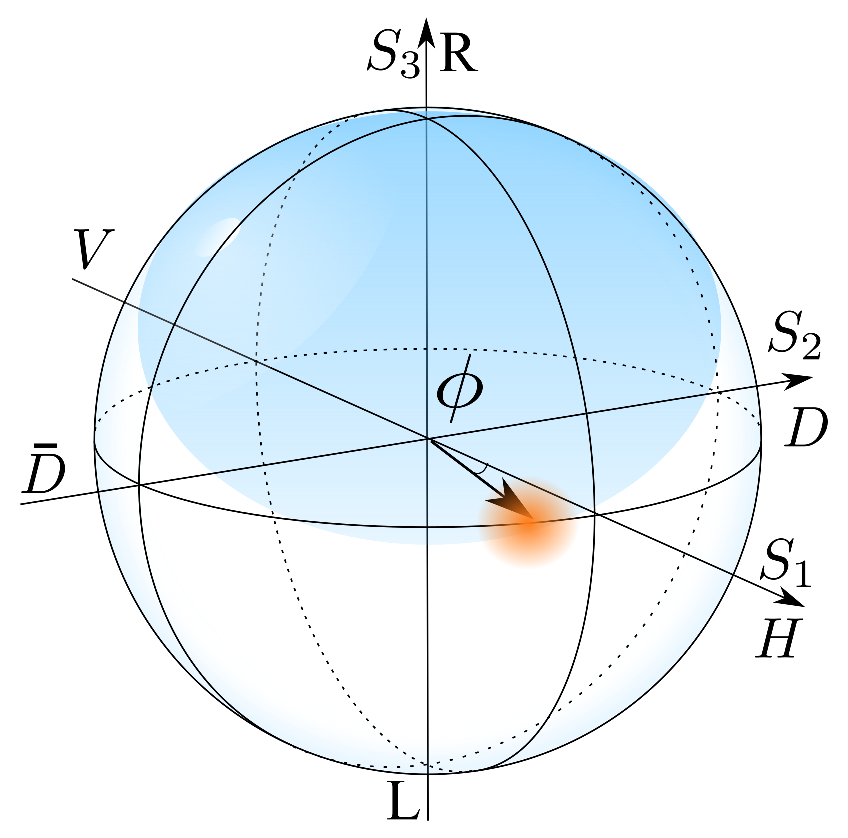
\includegraphics[width=0.55\textwidth]{../media/Figs/poincaresphere_initialS1_Faradayrot_crystal}}
   \caption[Polarization represented on the \Poincare sphere.]{\Poincare sphere and Stokes vector representation of the polarization of light. A state of polarization of the light can be represented as a vector $ \mathbf{S}=(S_0,S_1,S_2,S_3) $ with the $ S_0 $ Stokes parameter proportional to the total photon flux defining the radius of the sphere. Along the axes, $ S_1 $ direction corresponds a linearly polarized light along the $ x $ axis (labeled with $ H $), $ S_2 $ direction a linearly polarized light along the diagonal direction $ 45^\circ $ from the $ x $ axis on the $ xy $ plane (labeled with $ D $), and $ S_3 $ direction a right-circularly polarized light (labeled as $ R $). Any points on the equator of the sphere are linearly polarized states. The north and south poles are circularly polarized states. Anywhere else are elliptically polarized states. }
   \label{fig:Poincaresphere}
\end{figure}

Similarly, in the circular polarization basis $ (\mathbf{e}_+,\mathbf{e}_-) $, the Stokes vector components can be given by
\begin{subequations}\label{eq:S_circularbasis}
\begin{align}
S_0 &= |\mathbf{e}_+^*\cdot \mathbf{E}|^2+|\mathbf{e}_-^*\cdot \mathbf{E}|^2 =E_+^2+E_-^2\\
S_1 &= 2\re\left[ (\mathbf{e}_+^*\cdot \mathbf{E})^*(\mathbf{e}_-^*\cdot \mathbf{E})\right] = 2E_+E_-\cos(\delta_--\delta_+)\\
S_2 &= 2\im\left[ (\mathbf{e}_+^*\cdot \mathbf{E})^*(\mathbf{e}_-^*\cdot \mathbf{E})\right] =2E_+E_-\sin(\delta_--\delta_+)\\
S_3 &= |\mathbf{e}_+^*\cdot \mathbf{E}|^2-|\mathbf{e}_-^*\cdot \mathbf{E}|^2 =E_+^2-E_-^2 %=E_L^2-E_R^2
\end{align}
\end{subequations}
 %(\qxd{Note: should the $S_3$ be $ E_R^2-E_L^2 $ instead?})
The Stokes vector components are independent from the choice of basis. 
One can choose another set of linear polarization basis, namely, the diagonal polarization basis or $ (\mathbf{e}_D,\mathbf{e}_{\thickbar{D}}) $ basis with 
\begin{subequations}\label{eq:eDeDbar}
\begin{align}
\mathbf{e}_D &= \frac{1}{\sqrt{2}} (\mathbf{e}_x+ \mathbf{e}_y)\\
\mathbf{e}_{\thickbar{D}} &= \frac{1}{\sqrt{2}} (\mathbf{e}_y - \mathbf{e}_x)
\end{align}
\end{subequations}
that is a $ 45^\circ $ rotation from the $ (\mathbf{e}_x,\mathbf{e}_y) $ Cartesian basis in the $ xy $ plane. The $ \mathbf{E} $ vector can then be written as  \begin{align}
\mathbf{E} = \mathcal{E}_D\mathbf{e}_D + \mathcal{E}_{\thickbar{D}}\mathbf{e}_{\thickbar{D}}=E_De^{i\delta_D}\mathbf{e}_D + E_{\thickbar{D}}e^{i\delta_{\thickbar{D}}}\mathbf{e}_{\thickbar{D}} .\label{eq:E_Dbasis}
\end{align}
Plugging Eqs.~\eqref{eq:eDeDbar} and~\eqref{eq:E_Dbasis} into Eq.~\eqref{eq:S2_xybasis}, one can find that in the diagonal polarization basis
\begin{align}\label{eq:S2_Dbasis}
S_2 = E_D^2-E_{\thickbar{D}}^2.
\end{align}
%\qxd{(Comment: why not $ E_{\thickbar{D}}^2-E_{D}^2 $?)}
Based on the expressions of Stokes vectors in different bases or Eqs.~(\ref{eq:S_xybasis},~\ref{eq:S_circularbasis} and~\ref{eq:S2_Dbasis}), we can find the relation between those Stokes vector components and the intensity of field components $ E_i^2 $ in different bases as below
\begin{subequations}\label{eq:S_intensitydiff}
\begin{align}
S_0 &= E_H^2+E_V^2 = E_+^2+E_-^2 = E_D^2+E_{\thickbar{D}}^2\\
S_1 &= E_H^2-E_V^2\\
S_2 &= E_D^2-E_{\thickbar{D}}^2\\
S_3 &= E_+^2-E_-^2 %=E_L^2-E_R^2
\end{align}
\end{subequations}
Above, we have replaced $ x\rightarrow H $ and $ y\rightarrow V $.
Given the intensity components $ E_i^2 (i=H,V,L,R,D,\thickbar{D})$ are proportional to the photon fluxes of the linear and circular polarization components, $ S_0 $ is proportional to the total flux of the light, $ S_1 $ is proportional to the photon flux difference in the $ x $- and $ y $-polarization components, $ S_2 $ is proportional to the photon flux difference of the $ D $- and $ \thickbar{D} $-polarization components, and $ S_3 $ is proportional to the photon flux difference of the $ L $- and $ R $-polarization components of the light. 
Given the total photon flux of the light, one can use waveplanes and beam splitters to decompose field components and pairs of photon detectors that measure the photon flux in orthogonal polarization bases to find the normalized Stokes vector components and hence measure the polarization state of the light. 
This defines the \emph{polarization spectroscopy technique}\index{polarization spectroscopy}~\cite{Deutsch2010a,Salvail2013}.

\subsection{Polarization spectroscopy on waveguide interfaces}
In this dissertation, we will be focusing on the atom-light interfaces with nanophotonic waveguides. 
We assume the waveguide is designed so that the polarization of a transverse light beam in free space is adiabatically coupled to a unique mode of the waveguide when the light travels through the waveguide; when the light exits the waveguide, modes of the waveguide can again adiabatically recover to a unique polarization state of a transverse light in free space. The map of free-space polarization state of the light and the internal modes of the waveguide identically applies to the incidence and emergence processes. A tapered nanofiber, for example, is designed to work in this way~\cite{Nayak2007}. We also assume the dispersive and distortion effects solely due to the waveguide has been compensated before the polarization state measurement or can be extracted out from the measurement result for us to only discuss the effects caused by atom-light interaction in the nanophotonic waveguide region. As a result, we can label the modes by the polarization state of the light that is adiabatically connected to. For instance, an $ H $ mode of a nanofiber indicates the mode adiabatically connected to a linearly polarized incident light with the polarization direction along the $ x $ or $ H $ axis. To study how the atom-light interaction changes the polarization state of the light, one could only measure the state of light in the free space, and hence the same method of polarization spectroscopy technique can be applied to the waveguide platform. A typical polarization spectroscopy experimental setup is illustrated in Fig.

\begin{figure}[ht] % Poincare sphere.
   \centering\makebox[\textwidth]{
   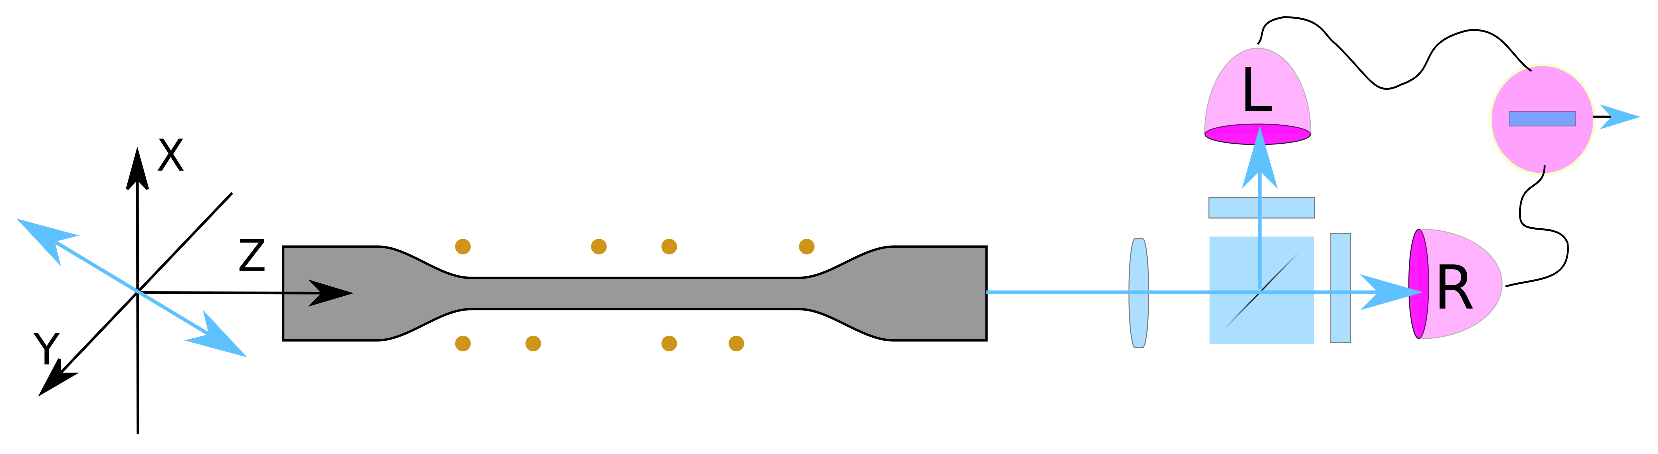
\includegraphics[width=0.85\textwidth]{../media/Figs/ProbeNanofiber_birefringence_lightpath_inputlight}}
   \caption[Polarization spectroscopy on a nanofiber platform.]{This figure shows an example of polarization spectroscopy scheme to measure the birefringence effect (see text) due to atom-light interaction near an optical nanofiber. A linearly polarized light polarized along the $ D $ direction (in blue) is incident to the tapered fiber and converted to the fiber's $ D $ mode that interacts with the atoms trapped near the surface of the waveguide. Due to the atom-light interaction, the state of polarization of the exit light is changed and can be measured with photon detectors. Shown in the figure, two photon detectors measuring the photon flux difference between the $ R $-polarized and $ L $-polarized light components is readout to indicate how much birefringence effect has been accumulated through the atom-light interaction. The measurement result can be mapped to a rotation of the Stokes vector $ \mathbf{S}=(S_0,S_1,S_2,S_3) $ on the \Poincare sphere. }
   \label{fig:polarizationspectroscopy}
\end{figure}

Although we will keep as general as possible, we will only look at single-mode waveguides that only allow degenerate fundamental modes to propagate, for simplicity reasons. The rest of this dissertation will be focusing on the atom-light interaction in the nanophotonic waveguide region and design quantum protocols for particular measurement schemes. There are two basic effects of the light response to be introduced in the following section: the \emph{birefringence effect}\index{birefringence effect} and the \emph{Faraday effect}\index{Faraday effect}.


\subsection{Birefringence and Faraday effects caused by atom-light interactions}
Let's first step back a little bit. 
For a completely polarized light\footnote{A partially polarized light satisfies $ S_0^2>S_1^2+S_2^2+S_3^2 $. For the ``natural light" or completely unpolarized light, the Stokes parameters satisfy $ S_1=S_2=S_3=0 $. Such, the degree of polarization is defined by $ R=\frac{\sqrt{S_1^2+S_2^2+S_3^2}}{S_0} \le 1$. Throughout this dissertation work, the degree of polarization is not our concern, and we assume the \Poincare sphere is properly normalized.}, they satisfy the relation~\cite{Born1999Principles}
\begin{align}
S_0^2=S_1^2+S_2^2+S_3^2
\end{align}
to fix one degree of freedom of the Stokes vectors. That leaves three independent variables to specify the $ \mathbf{S} $ vector of the polarization state of a light.
For example, in the linear polarization basis, $ E_x $, $ E_y $ and $ \delta_x-\delta_y $ uniquely define the polarization state of the light, where the phase difference between the two linear components of the field, $ \phi=\delta_x-\delta_y $, determines the helicity and the amplitudes of the two field components determine polarization magnitude and the polarization angle from the $ x $ axis. Similar rule applies to polarization representations with other bases and more complicated light patterns~\cite{Mecozzi2011Unified}. On the \Poincare sphere, $ (S_1,S_2,S_3) $ can be specified by the orientation angle $ \Psi (0\le \Psi \le \pi) $ of the ellipse, another angle $ \Theta (-\frac{\pi}{4}\le \Theta \le \frac{\pi}{4}) $ which characterizes the ellipticity and the sense in which the ellipse is being described ($ S_0 $) by~\cite{Born1999Principles}
\begin{align}
S_1 &= S_0\cos(2\Theta)\cos(2\Psi)\\
S_2 &= S_0\cos(2\Theta)\sin(2\Psi)\\
S_3 &= S_0\sin(2\Theta).
\end{align}
The factor of 2 reflects the symmetry of polarization. For example, a linear polarization is said to be orientated on the positive $ x $ direction is the same as on the negative $ x $ direction. 

To specify a polarization state if the polarization magnitude or $ S_0 $ is fixed, we only need two free variables--$ \Theta $ and $ \Psi $, for example. On the \Poincare sphere, one can specify a state of polarization from a given initial state by two consequent rotations by two orthogonal axes, respectively. 
We define the rotation around the $ S_1 $, $ S_2 $ or arbitrary linear polarization axis is physically generated by the \emph{birefringence effect}\index{birefringence effect};
the rotation around the $ S_3 $ axis is generated by the \emph{Faraday effect}\index{Faraday effect}. 
With these two polarization rotation effects, one can generate arbitrary polarization state of light from an initial state. 

Consider a light beam propagates through a cloud of atoms and generates a birefringence rotation on its polarization state. This process is possible if there is a relative speed difference of the light propagation along two orthogonal directions which are usually defined as the \emph{fast axis}\index{fast axis} and \emph{slow axis}\index{slow axis}. Correspondingly, the effective index of refraction due to the atom-light interaction along the two directions are different and denoted by $ n_f $ and $ n_s $ with $ 1\le n_f<n_s $, respectively. Therefore, there is a phase difference $ \phi $ after the light propagating by distance $ L $, where 
\begin{align}
\phi= k(n_f-n_s)L.
\end{align}
Consequently, a linearly polarized light input may become elliptically polarized after the interaction, and this phase difference above indicates how much the Stokes vector is rotated from a linear polarization axis on the \Poincare sphere define by the orientation of the fast axis.
Physically, how much the phase shift is generated due to the light components along the fast and slow axes due to the interaction with atoms determines how strong the birefringence effect is. 
Given a thickness of the atom cloud, if a linear polarization component of the light along the $ x $ axis gives the maximum phase shift after the interaction among all the other linear polarization components while the $ y $ component yields the minimum phase shift, then the $ x $ axis and the $ y $ axis define the fast axis and slow axis, respectively. Then the interaction will yield a birefringence effect of rotating the Stokes vector around the $ S_1$ axis on the \Poincare sphere. 

Similar to Eq.~\eqref{eq:S_intensitydiff}, one can generalize the physics explanation of birefringence effect due to a cloud of atoms to both birefringence and Faraday effects due to atoms trapped nearby a waveguide by looking at the phase shift difference between two orthogonal modes.
Let us consider all atoms trapped outside of a waveguide can be projected to the same position on the transverse plane of the fiber profile up to a mirror reflection symmetry across the fiber axis, which is true for the tapered nanofiber experiments with atoms trapped on an optical lattice~\cite{Dawkins2011,Vetsch2010Optical}. 
For instance, if both the $ H $ mode and $ V $ mode at the atoms' position yield the same light phase shift while the $ R $ mode and $ L $ mode yield different phase shifts, then the atom-light interaction will yield a Faraday effect which is a polarization rotation around the $ S_3 $ axis on the \Poincare sphere.

In general, as a result of the atom-light interaction, the polarization of the light will experience one of the two optical effects, the birefringence effect and the Faraday effect, or a mixture of the two effects. If we denote the polarization state of the light by $ \ket{\phi} $ and quantize the Stokes vector as a quantum operator $ \hat{\mathbf{S}}=(\hat{S}_0;\hat{S}_1;\hat{S}_2;\hat{S}_3) $ as a column vector operator, the rotation of the polarization of the light on the \Poincare sphere due to the interaction with atoms can be denoted as
\begin{align}
e^{i\boldsymbol{\chi}\cdot\hat{\mathbf{S}} }\ket{\phi},
\end{align}
where the vector $ \boldsymbol{\chi}=(\chi_0,\chi_1,\chi_2,\chi_3) $ are the rotation angles around $ S_i (i=1,2,3) $ axes and the photon number attenuation on $ S_0 $. The strength and details of the atom-light interactions hide in the $ \boldsymbol{\chi} $ vector. The key to designing particular polarization-based interactions lay on the phase response of particular waveguide modes. With this brief introduction of the polarization rotations and waveguide setups, we will dive into the beauty of atom-light interactions and inspire non-classical applications in the rest of the dissertation.

In the next section, we will step into the properties of the bare waveguide modes and the dispersive response of the waveguide modes due to the presence of the atoms from the perspective of Green's function approach.

\section{Dispersive light response in the perspective of Green's function approach}
\subsection{Eigenmodes of a dielectric waveguide}\label{sec:eigenmodesofwaveguides}
We assume that the waveguide we are going to study is infinitely long and has a uniform profile of refractive index through the fiber axis. For a nanophotonic waveguide that can trap atoms using its evanescent field, its dimension of the cross-section is smaller than the wavelength $ \lambda $ of the trapping field (typically, a quasi-monochromatic laser beam operating around $ \lambda=894 $nm or $852  $nm which are the D1 and D2 lines of the cesium atoms considered in the numerical simulations later in this dissertation). 
We assume the waveguide is a linear medium with no absorption to the traveling wave. The refractive bulk index\index{refractive index} of the waveguide can be given by
\begin{align}
n_0(\br_\perp) = \begin{cases} 
n_1(\br_\perp), &\quad \text{core region},\\
n_2(\br_\perp), &\quad \text{clad},
\end{cases} 
\end{align}
where $ n_1>n_2 $, $ \br_\perp=(x,y) $ is the coordinate in the transverse plane of the waveguide, and the index of refraction defined above applies to all transverse slices along the $ z $ axis which is the waveguide axis along the light propagation direction.

For a typical optical nanofiber as an example, it has a cylindrical cross-section with a radius $ a $. We use $ a=225 $nm, $ n_1=1.4496 $ as a constant in the core region ($ r_\perp\le a $) and $ n_2=1.0000 $ in vacuum clad region ($ r_\perp>a $), where we have set the $ z $ axis to be the symmetric center of the nanofiber and $ r_\perp =\sqrt{x^2+y^2} $.
Another nanophotonic waveguide we are going to utilize is a \SWG, which has a square cross-section of the waveguide core with a width of $ w=300 $nm, $ n_1=2.0 $ for an ideal Si$_3$N$_4$ core medium $ (|x|\le w/2,|y|\le w/2) $, and the clad is also vacuum. 
In both cases, only the fundamental guided modes are allowed to propagate through the waveguide. That is the allowed guided modes have a single propagation constant\index{propagation constant} or projected wavenumber $ \beta_0 \,(n_1k_0<\beta_0<n_2k_0)$ with wavenumber\index{wave number} $k_0=2\pi/\lambda=\omega_0/c $, where $\omega_0$ is the angular frequency of the electric field, and $ c $ is the speed of light in vacuum. 
A monochromatic electric field propagating in such a waveguide can be given by~\cite{Jackson1975}
\begin{equation}
\mathbf{E}_0(\br,t)=\boldsymbol{\mathcal{E}}_0(\br_\perp)e^{i(b\beta_0 z-\omega_0 t)} %+\frac{1}{2}\mathrm{c.c.}
=\mathcal{E}_0\mathbf{u}_0(\br_\perp)e^{i(b\beta_0 z-\omega_0 t)}, %+\frac{1}{2}\mathrm{c.c.},
\label{Ert0}
\end{equation}
where $ b=\pm $ indicating the propagating direction, and $\boldsymbol{\mathcal{E}}_0(\br_\perp)=\mathcal{E}_0\mathbf{u}_0(\br_\perp)$ is the positive-frequency electric field envelope,
with $\mathcal{E}_0$ determining the field amplitude and $\mathbf{u}_0(\br_\perp)$ as the polarization vector at $ \br_\perp=(x,y)=(r_\perp,\phi) $ in either Cartesian or cylindrical coordinate system.
In general, $\mathcal{E}$ is a complex scalar constant and $\mathbf{u}(\br_\perp)$ is a complex vector normalized to the energy flux or power across a transverse plane. The spatial dependent part of the field $ \mathbf{u}(\br_\perp)e^{ib\beta_0 z} $ can be written as a linear combination of the \emph{eigenmodes}\index{eigenmode} that are supported by the waveguide.
The fundamental modes of the nanofiber are the \HE modes with the degeneracy of propagation directions $ b=\pm $ and polarizations of two labeled by $ p $. For the single-mode \SWG, the quasi-\TE and the quasi-\TM modes together with degeneracy of propagation directions and polarizations of two. We use subscript $ \mu={j,\beta,p} $ to indicate a generic guided eigenmode, $ \mathbf{u}_\mu (\br) $, where $ j=1 $ and $ \beta=\beta_0 $ for the single-mode waveguides. Those eigenmodes satisfy the orthogonality condition,
\begin{align}
\int d^2 \mbf{r}_\perp \, n^2(r_\perp)\mathbf{u}^*_\mu (\br_\perp) \cdot \mathbf{u}_{\mu'} (\br_\perp)\big|_{\beta = \beta'} = \delta_{j,j'}\delta_{p,p'},
\end{align}
and have units $1/\sqrt{A}$, where $ A $ is area~\cite{LeKien2014}.
The degeneracy of polarizations of the \HE modes allow one to write the eigenmodes of the nanofiber on arbitrary polarization basis. Two convenient guided-mode bases are the quasilinear and quasicircular polarization modes. In Figs.~\ref{fig:Modes_Rot45HV_fiber} and~\ref{fig:Modes_Rot45LR_fiber}, we show the decomposition of a diagonally polarized $ D $ mode of a nanofiber in the $ HV $- and $ LR $-bases, respectively. From the figures, if we place an atom on the $ x $ axis, we find that the $ H $ mode component has a much stronger intensity at the atom position than the $ V $ mode component. This property of \emph{mode isotropy}\index{isotropy of waveguide modes} on azimuthal directions is intrinsic for the waveguides but doesn't exist in free propagating fundamental Gaussian laser beams that have been typically used in atom-light coupling experiments. In contrast, the decomposed $ R $ and $ L $ modes at the atom position have the same intensity. As we will see later, how to choose a good mode basis based on the atomic internal structure and fully utilize the isotropic property of the waveguide modes is the key to optimally designing some quantum operations on the atoms for wide applications, which yields great advantages of the nanophotonic waveguides over the atom-light quantum interface in vacuum. For now, we have to hold our breath to pave some necessary foundations.

\begin{figure}
\centering\makebox[\textwidth]{
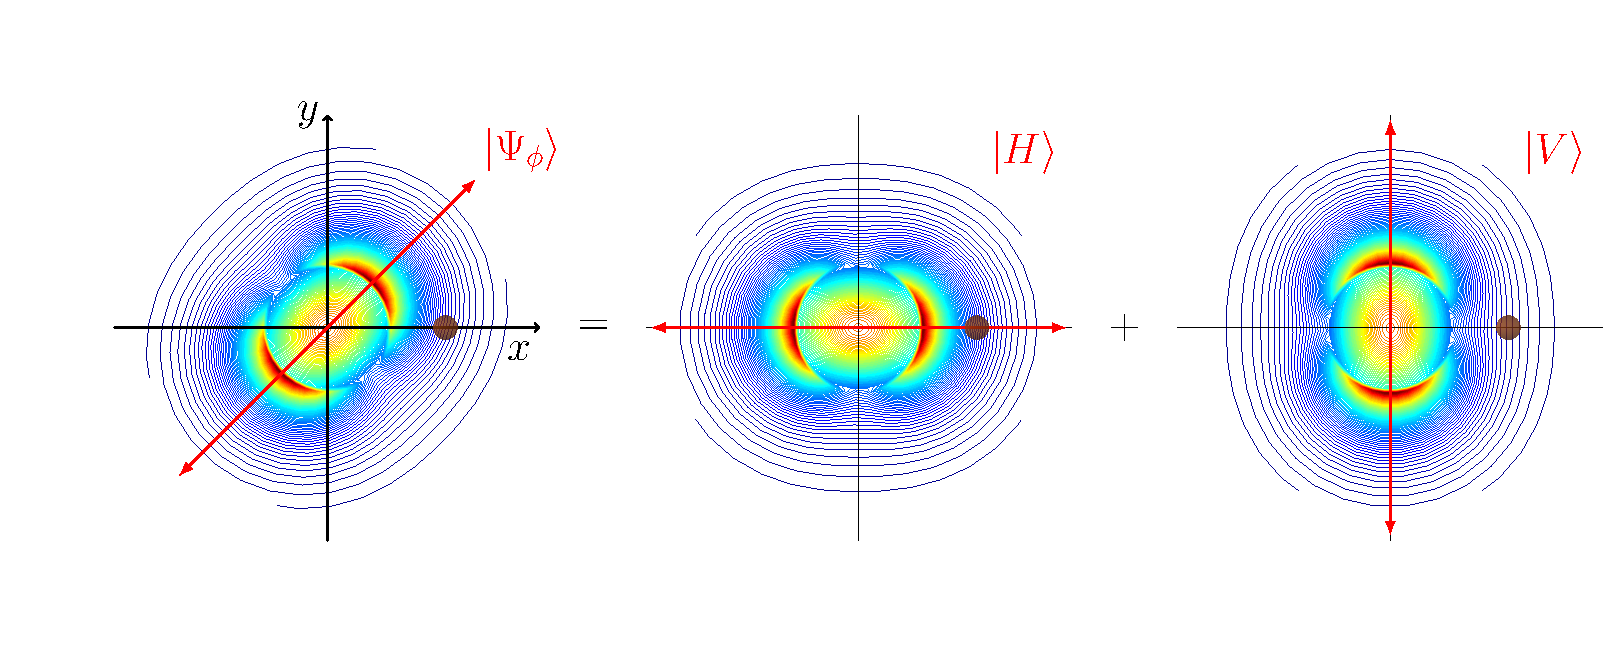
\includegraphics[width=12cm]{../media/Figs/Modes_Rot45HV}}
\caption[Mode decomposition of an input quasilinear polarized laser beam in the $ |H\rangle $ and $ |V\rangle $ mode basis.]{Mode decomposition of an input quasilinear polarized $ D $ ($ \ket{\Psi_\phi}=\ket{D} $) mode. The $ D $ mode is formed by shining an input laser beam polarized along the bisection between $ x $  and $ y $ axes. It is equivalent to have one $ H $ ($ |H\rangle $) mode and one $ V $ ($ |V\rangle $) mode with input polarized along the $ x $ axis and $ y $ axis, respectively. Shown in color are the equal-potential lines of the intensities of the modes. The dark dot indicates an possible atom position on the $ x $ axis, where the intensity of the $ H $ mode is much larger than the $ V $ mode.  }\label{fig:Modes_Rot45HV_fiber}
\end{figure}

\begin{figure}
\centering\makebox[\textwidth]{
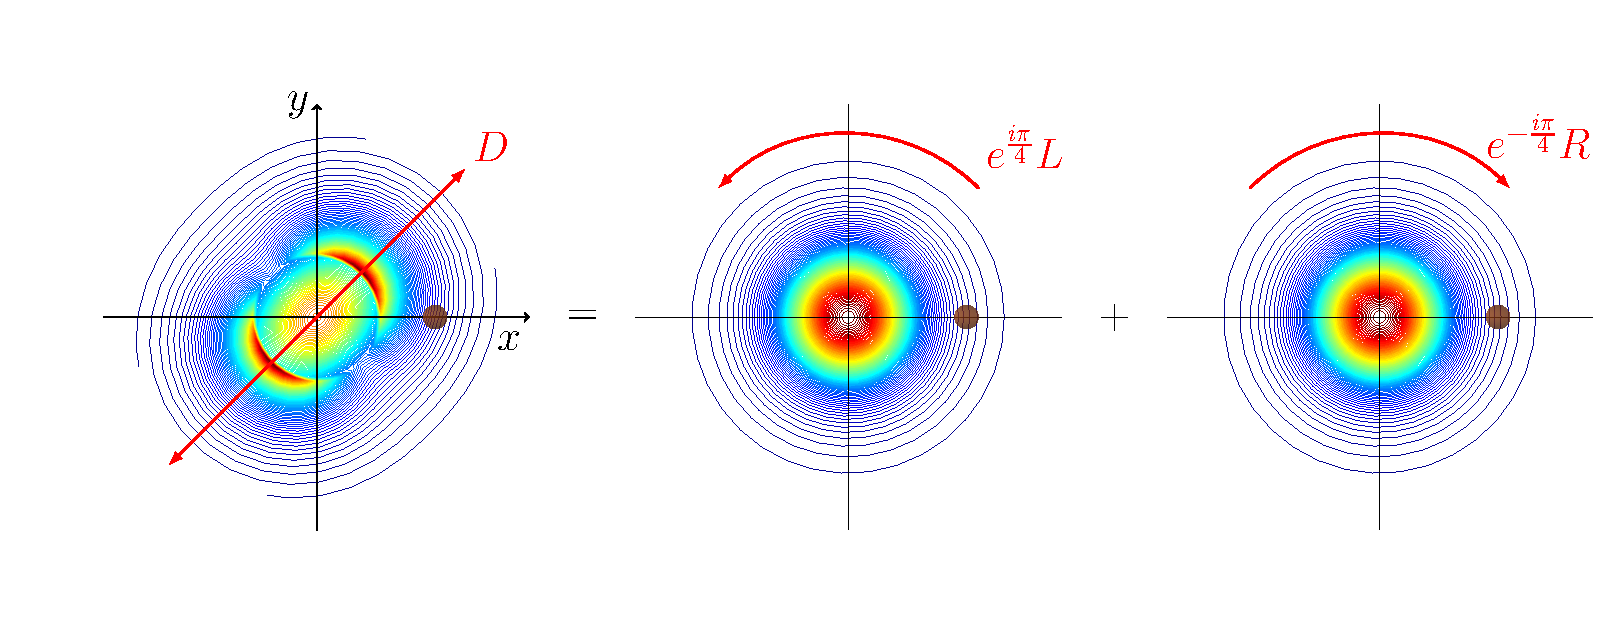
\includegraphics[width=12cm]{../media/Figs/Modes_Rot45LR}}
\caption[Mode decomposition of an input quasilinear polarized laser beam in the $ L $ ($ |L\rangle $) and $ R $($ |R\rangle $) mode basis.]{Same as Fig.~\ref{fig:Modes_Rot45HV_fiber} but decomposed into the $ LR$-mode basis. At the dark dot's position, the $ L $ and $ R $ modes have the same intensity.}\label{fig:Modes_Rot45LR_fiber}
\end{figure}

The quasi-\TE and quasi-\TM modes are eigenmodes of the \SWG with orthogonal polarizations and can be adiabatically connected to the $ x $- and $ y $-polarized linear free-space light inputs. Therefore, we can define the quasi-\TE and quasi-\TM modes as the $ H $ and $ V $ modes for the \SWG geometry. They have similar anisotropic properties as the fiber modes do.

The eigenmodes of a waveguide, in complete cases, should include both the guided (bounded) and radiation (unbounded or unguided) solutions, based on the corresponding waveguide boundary condition problem governed by the Maxwell equations~\cite{Jackson1975}. Below, we will only sketch out the condition to divide the guided and radiation modes using an analogy to the \sch equation, which will be useful to understand the radiation decompositions in sections follow.

\subsubsection{Guided and radiation modes}
If we want to fully calculate the eigenmodes of a waveguide, we need to consider both the electric and magnetic fields, the spatial parts of which are governed by the wave equations
\begin{align}\label{EBz}
\left(\nabla^2 +k^2 \varepsilon(\br_{\perp})\right) \begin{pmatrix}
\mathcal{E}_z(\br)\\
\mathcal{B}_z(\br)
\end{pmatrix} = 0,
\end{align}
where $ \varepsilon=n^2 $ is the permittivity of the medium and $ k $ is the wavenumber of the modes. The equation above is derived from the \emph{Maxwell-Helmholtz equation}\index{Maxwell-Helmholtz equation}, for example, for electric field part that
\begin{align}
\left[ -\nabla\times\nabla\times+\frac{\omega^2}{c^2}n^2(\br) \right] \boldsymbol{\mathcal{E}}(\br) &=0. \label{MaxwellHelmholtz0}
\end{align}
Notice that we only concentrate on the $ z $-component of the fields since all the other components can be expressed in terms of the $ z $-components of the fields (see detailed derivations in Appendix~\ref{MWE:components} in the cylindrical coordinate system). 

We use an ansatz that 
\begin{align}
\mathcal{E}_z (r_\perp, \phi, z) &= \psi(r_\perp,\phi) e^{i\beta z}\\
\mathcal{B}_z (r_\perp,\phi,z) &= \zeta(r_\perp,\phi) e^{i\beta z}.
\end{align}
Substituting the above into Eq.~\ref{EBz}, we obtain
\begin{align}\label{psizeta}
\left(\nabla^2_\perp +(k^2 \varepsilon(\br_{\perp})-\beta^2 )\right) \begin{pmatrix}
\psi(r_\perp,\phi)\\
\zeta(r_\perp,\phi)
\end{pmatrix} = 0.
\end{align}
Now, the problem of solving a three dimensional wave equation for $ \boldsymbol{\mathcal{E}} (r_\perp, \phi, z) $ 
and $ \boldsymbol{\mathcal{B}} (r_\perp, \phi, z)$ turns into a problem of solving a two-dimension differential 
(mode) equation for $ \psi(r_\perp,\phi) $ and $ \zeta(r_\perp,\phi) $. 

There are two special cases for the modes. If $ \psi=0 $ as a constant, which means there is no $ z $-component of the electrical field, then the propagating mode is called a TE mode\index{mode!TE mode}. Similarly, if $ \zeta=0 $ as a constant, which corresponds to zero magnetic $ z $-component, 
then this mode is called a TM mode\index{mode!TM mode}. However, in many waveguide geometries including the nanofiber case with a cylindrical symmetry, the modes cannot be grouped into TE and TM guided waves. In general, the modes with 
both electrical and magnetic nonzero $ z $-components are known as EH and HE hybrid 
modes\index{mode!HE mode}~\cite{Snyder1983Optical}--the second letter in the names indicates the field that has the dominance of the longitudinal component.

We focus on the electrical part for now. The magnetic field can be solved similarly. Eq.~\ref{psizeta} gives
\begin{align}\label{eigenpsi}
[\nabla^2_\perp + k^2\varepsilon(r_\perp)] \psi(r_\perp, \phi) = \beta^2\psi(r_\perp,\phi).
\end{align}
Compared to the time-independent \sch equation
\begin{align}
\left[\frac{\hat{P}^2}{2m}+V(\hat{\mathbf{r}}_\perp) \right] \psi(\br_\perp)&= E\psi(\br_\perp)\\
\text{or}\quad \left[ \nabla^2_\perp -V(r_\perp) \right] \psi (r_\perp, \phi) &= -E\psi(r_\perp,\phi),
\end{align}
we can conclude that the mode equation (Eq.~\ref{eigenpsi}) is basically an eigenvalue equation for the \sch wavefunctions if we make the replacement
\begin{align}
V_{ef\!f}=-k^2\varepsilon(\br\!_\perp) &\sim V(\br\!_\perp)\\
-\beta^2 &\sim E.
\end{align}
With these analogies, we can find that the guided modes dictated by the wave equation should correspond to the bounded eigenstates of the trapping potential problem obeying to the \sch equation; likewise, the radiation modes of the wave equation correspond to unbounded states in the scattering problem following the \sch equation. In details, for the time-independent \sch problem, if $ 0<E\leq V $, then the eigenstates are bounded and have discrete solutions with respect to $ E $; if $ E>V $, then the resulted states is unbounded and have continuous solutions of energy. For the waveguide's eigenmodes, similarly, we can also use the relative position of $ V_{ef\!f} $ and $ -\beta^2 $ to classify the bound and radiation modes. 

Let us consider the concrete case of a nanofiber with step-function-like permittivity as a function of $ r_\perp $. The analogy of trapping potentials of the wave equation is illustrated in Fig.~\ref{Figs/scatteredmode}. In the regime $ n_2k<\beta<n_1k $, the eigenmodes have discrete solutions with respect to $ \beta $, which yield $ \beta=\beta_0 $ for a single-mode fiber; in the $ 0<\beta<n_2k $ regime, the eigenmode solutions are continuous with respect to $ \beta $. Similar result applies to the \SWG case. 

%\scalefig{Figs/scatteredmode}{0.8}{Bound and unbound states for the nanofiber eigenvalue 
%problem. $ \varepsilon(r\!_\perp)=\varepsilon_{f} =n_1^2$ if $ r_\perp < a $; otherwise, $\varepsilon
%(r\!_\perp) =1 $. The parameter $ a $ is the radium of the nanofiber. } 

\begin{figure}
\centering\makebox[\textwidth]{
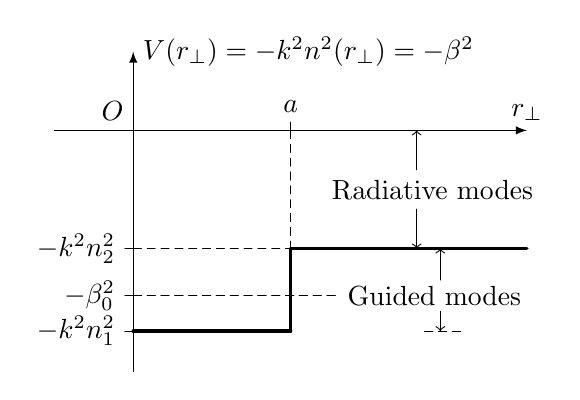
\begin{tikzpicture}[scale=1,cap=round]
% Configurable parameters
\def\k{1.5cm}
\def\eps{1.5*1.7cm}
\def\betasq{1.5*1.4cm}
\def\a{2cm}
\def\maxr{5cm}

% Styles
\tikzstyle{axes}=[arrows={-latex}]
\tikzstyle{auxline}=[densely dashed]
\tikzstyle{important line}=[very thick]

% Coordinates and points.
\coordinate (O) at (0,0);	% Origin.
\coordinate (A) at (\a,0);	% The surface distance to the axis of the fiber.
\coordinate (B) at (0,-\eps);	% -k^2\epsilon at the center of the fiber.
\coordinate (C) at (\a,-\eps);	% -k^2\epsilon on the surface of the fiber.
\coordinate (D) at (0,-\betasq);	% -\beta^2 point at the center of the fiber.
\coordinate (E) at (\a*1.3,-\betasq);	% -\beta^2 point at the end of the maximum r.
\coordinate (F) at (0,-\k);	% -k^2 point at the center of fiber.
\coordinate (G) at (\a,-\k); 	% -k^2 point on the surface of the fiber.
\coordinate (H) at (\maxr,-\k); 	% -k^2 point at the end of r.

% The graphic
 % help grid
% \draw[style=help lines,step=0.5cm] (-2.0,-2.0) grid (2.0,2.0);
  
% Draw axes and marks.
\draw [axes] (-1cm, 0) -- (\maxr,0) node [above] {$r_{\perp}$};
\draw [axes] (0, -1.2*\eps) -- (0, 1.0cm) node [right] {$V(r_{\perp})=-k^2n^2(r_{\perp})=-\beta^2$};
\draw (O) node [above left] {$O$};
\draw[thin] (A) -- (\a,3pt) node[anchor=south] {$a$}; 
\draw (B) -- (-3pt,-\eps) node[anchor=east] {$-k^2n_1^2$};
\draw (D) -- (-3pt,-\betasq) node[anchor=east] {$-\beta_0^2$};
\draw (F) -- (-3pt,-\k) node[anchor=east] {$-k^2n_2^2$};

% Draw potential lines.
\draw[important line] (B) -- (C);
\draw[important line] (C) -- (G);
\draw[important line] (G) -- (H);
\draw[auxline] (D) -- (E) node[right] {Guided modes};
\draw[auxline,very thin] (F) -- (G);
\draw[auxline,very thin] (A) -- (G);

% Other labels and auxlines.
%\draw[<->] (\a*1.25,0) -- (\a*1.25,-\k) node[midway,right] {Scattered modes};
\draw (\a*1.2,-\k/2) node[right] {Radiative modes};
\draw[<-] (\a*1.8,0) -- (\a*1.8,-0.5cm);
\draw[->] (\a*1.8,-1cm) -- (\a*1.8,-\k);
\draw[<-] (\a*1.95,-\k) -- (\a*1.95,-\k-0.4cm);
\draw[->] (\a*1.95,-\k-0.8cm) -- (\a*1.95,-\eps);
\draw[auxline] (\a*1.85,-\eps) -- (\a*2.08,-\eps);
\end{tikzpicture}
}
\caption[Trapping potential analogy of the bounded and unbounded modes of a nanofiber.]{Bound and unbound states for the fiber eigenvalue problem. $ \varepsilon(r\!_\perp)=\varepsilon_{f} =n_1^2$ if $ r_\perp < a $; otherwise, $\varepsilon(r\!_\perp) =1 $. The parameter $ a $ is the radius of the nanofiber.}
\label{Figs/scatteredmode}
\end{figure}

The division of guided and radiation modes based on the value of $ \beta $ can also be roughly understood in the perspective of geometric optics as elucidated in Fig.~\ref{fig:Fibermodes}. We regard $ \beta $ as the $ z $-projected wave number of a wave vector of the light ray on $ \vec{k} $ direction. If the ray is incident in an angle that satisfies the total internal reflection condition (in our case, $ k_0<\beta<n_1k_0 $ with $ n_2=1 $), the corresponding modes are guided; otherwise, the modes are unguided with the light leaking out and decaying along $ z $.

\begin{figure}
\centering\makebox[\textwidth]{
\begin{tikzpicture}[scale=1,cap=round]
% Configurable parameters
\def\fiberrad{1cm}	% Radius of the nanofiber.
\def\comprad{0.45cm}	% Compressed radius of the nanofiber in the view angle.
\def\fiberleftx{0}	% The x-coordiante of the center of the left surface of the fiber.
\def\fiberlefty{0}	% The y-coordiante of the center of the left surface of the fiber.
\def\fiberlength{6.6cm} % The length of the fiber.

% Styles
\tikzstyle{axes}=[arrows={-latex}]
\tikzstyle{auxline}=[densely dashed]
\tikzstyle{important line}=[thick]
\tikzstyle{dot}=[circle,inner sep=1pt,fill,label={#1},name=#1]

% Coordinates and points.
\coordinate (O) at (0,0);	% Origin.
\coordinate (LO) at (\fiberleftx,\fiberlefty); % Center of the left-side surface of the nanofiber.
\coordinate (RO) at (\fiberleftx+\fiberlength,\fiberlefty); % Center of the right-side surface
\coordinate (A) at ({\fiberleftx},{\fiberlefty+\fiberrad});	% Top-left point of the nanofiber.
\coordinate (B) at ({\fiberleftx+\fiberlength},{\fiberlefty+\fiberrad});	% Top-right point of the nanofiber.
\coordinate (C) at ({\fiberleftx+\fiberlength},{\fiberlefty-\fiberrad});	% Bottom-right point of the fiber.
\coordinate (D) at ({\fiberleftx},{\fiberlefty-\fiberrad});	% Bottom-left point of the nanofiber.

% The graph.
% help grid
% \draw[style=help lines,step=0.5cm] (-2.0,-2.0) grid (2.0,2.0);

% Draw the fiber.
\begin{scope} 
    % Outer edge.
    %\fill[left color=purple!50!black,right color=purple!50!black,middle 
%color=purple!50,shading=axis,opacity=0.25] (A) -- (B) arc (90:270:{\comprad} and {\fiberrad}) -- (D) arc 
%(270:90:{\comprad} and {\fiberrad});
    % Right-side surface.
    %\fill[top color=purple!90!,bottom color=purple!2,middle color=purple!30,shading=axis,opacity=0.25] 
%(RO) circle [x radius={\comprad}, y radius = {\fiberrad}];
    % Draw lines of all edges.
    \draw (A) -- (B);
    \draw  (RO) circle [x radius = {\comprad}, y radius =  {\fiberrad}];
    \draw (C) -- (D) arc (270:90:{\comprad} and {\fiberrad}); 
    \draw[densely dashed] (A) arc (90:-90:{\comprad} and {\fiberrad});
\end{scope}

% Draw the guide mode wave vector and propagation lines.
% First part of the ray: up-solid line.
\draw[red] (O)--(2.0*\fiberrad,\fiberrad);
%\draw[red,decoration={ markings,  % This schema allows for fine-tuning the arrows.
%      mark=at position 0.5 with {\arrow{latex'}}, 
%      mark=at position 0.82 with {\arrow{latex'}}},postaction={decorate}] (O) -- (2.0*\fiberrad,\fiberrad)-- (6.0*\fiberrad,-\fiberrad);
% The penetration part of ray: dashed line.
\draw[red,densely dotted] (2.0*\fiberrad,\fiberrad) -- (2.3*\fiberrad,1.1732*\fiberrad) -- (2.6*\fiberrad,\fiberrad);
% The reflected part: solid downarrow.
\draw[red,decoration={ markings,  % This schema allows for fine-tuning the arrows.
      mark=at position 0.2 with {\arrow{latex'}}, 
      mark=at position 0.6 with {\arrow{latex'}}},postaction={decorate}] (2.6*\fiberrad,\fiberrad)-- (6.6*\fiberrad,-\fiberrad);
% The ruler part.
\draw[important line,-latex'] (O) --(27:1) node[below,xshift=8,yshift=5] {$ \vec{k} $};
\draw[auxline] (27:1) -- ({cos(27)},-1.5)  node [below] {$\beta_0$};

% Draw radiation modes.
% Radiation ray 1:
\draw[blue,decoration={ markings,  % This schema allows for fine-tuning the arrows. 
      mark=at position 0.95 with {\arrow{latex'}}},postaction={decorate}] (O) -- (0.5,\fiberrad) -- (1.5,\fiberrad*1.1);
\draw[-latex'] (O)--(63.5:1);
\draw[auxline] (63.5:1) -- ({cos(63.5)},-2);
% Radiation ray 2:
\draw[blue,decoration={ markings,  % This schema allows for fine-tuning the arrows. 
      mark=at position 0.95 with {\arrow{latex'}}},postaction={decorate}] (O) -- (0.4,\fiberrad) -- (1.4,\fiberrad*1.4);
\draw[-latex'] (O)--(68.5:1);
\draw[auxline] (68.5:1) -- ({cos(68.5)},-2);
% Radiation ray 3:
\draw[blue,decoration={ markings,  % This schema allows for fine-tuning the arrows. 
      mark=at position 0.95 with {\arrow{latex'}}},postaction={decorate}] (O) -- (0.25,\fiberrad) -- (0.9,\fiberrad*1.9);
\draw[-latex'] (O)--(76:1);
\draw[auxline] (76:1) -- ({cos(76)},-2);
% Radiation ray 3:
\draw[blue,decoration={ markings,  % This schema allows for fine-tuning the arrows. 
      mark=at position 0.95 with {\arrow{latex'}}},postaction={decorate}] (O)-- (0,2*\fiberrad);
\draw[-latex'] (O) -- (0,\fiberrad);
% Draw dots inbetween.
\draw[dotted] ([shift=(26:1)] 0.2,1.0*\fiberrad) arc (26:45:1);
\draw[dotted] ([shift=(60:1)] 0.1,1.0*\fiberrad) arc (60:89:1);

% Labels and denotes.
\draw (O) node[dot] {};
\draw (O) node[left] {O};
\draw[auxline,-latex] (O) -- (\fiberlength*1.0,0) node [above] {$ z $};	% Z axis line.
\draw[auxline] (0,\fiberrad) -- (0,-2);
\draw[important line,-latex] (0,-2) node[left] {$ 0 $}--(2.5,-2) node[right] {$ k_z $};% kz axis.
\draw (0,-2) -- (0,-2.08);
\draw (0.5,-2) -- (0.5,-2.08) node [anchor=north] {$k_0$};
\draw ({cos(27)},-2) -- ({cos(27)},-2.08);
\draw (1.1,-2) -- (1.1,-2.08) node [below right,xshift=-5] {$k_0n_1$};
\draw (3.35,-0.5) node[red] {Guided modes};	% Guided modes label.
\draw (2.7,1.7*\fiberrad) node[blue] {Radiative modes};	% Radiative modes label.
\end{tikzpicture}
}
\caption[Fiber modes classified through the $ z $-component of the wave vector, $ \beta $.]{Fiber modes classified through the $ z $-component of the wave vector, $ \beta $. We have assumed $ n_2=1 $ for a vacuum clad. From the diagram, we define $ \beta $ is the $ z $-projection of $ \vec{k} $, that is $ \beta=k\cos\theta $, where $ k $ is the length of the wave vector following the ray-trace of the light propagating in all directions, and $ \theta $ is the angle of the ray of light to the $ z $ axis. We see that when $ \theta $ is small or $ \beta $ is longer than some value, the light can satisfy the total internal reflection condition and hence the corresponding mode solution can be guided through the fiber; if $ \theta $ is large or $ \beta $ is small, then the light cannot satisfy the total internal reflection condition, and hence the corresponding modes are unguided or radiation leaking out of the fiber.}
\label{fig:Fibermodes}
\end{figure}

If we denote $ \mathbf{u}_\nu(r\!_\perp ) $ as the radiation mode with mode index $ \nu=(\omega,\beta,m,p) $, where $ m=0,\,\pm 1,\,\pm 2,\cdots $ is the mode index, and $p=\pm$ denotes the polarization pattern. The orthogonality conditions of the guided and radiation modes can be summarized below: 
\begin{align}
\int\mathrm{d}^2\br_\perp n^2(\br_\perp)|\mathbf{u}_{\mu}(r\!_\perp )|^2 &=1,\\
\int\mathrm{d}^2\br_\perp n^2(\br_\perp)\left[\mathbf{u}_{\nu}(r\!_\perp )\cdot\mathbf{u}_{\nu'}^*(r\!_\perp )\right]_{\beta=\beta',m=m'} &=\delta(\omega-\omega')\delta_{pp'}.
\end{align}
The completeness relationships of the modes can be given by
\begin{align}
\sum_{f,p}\int \mathrm{d}\mathbf{k} \,n^2(\br_\perp)\mathbf{u}_{\mu}(r\!_\perp )\mathbf{u}_{\mu}^*(r'\!_\perp ) &= \unittensor\delta^T(r\!_\perp-r'\!_\perp),\\
\sum_{m,p}\int \mathrm{d}\mathbf{k} \, n^2(\br_\perp)\mathbf{u}_{\nu}(r\!_\perp )\mathbf{u}_{\nu}^*(r'\!_\perp ) &=\unittensor\delta^T(r\!_\perp-r'\!_\perp),
\end{align}
where $ \unittensor $ is the unit tensor, and $\delta^T(r\!_\perp-r'\!_\perp)$ is the delta function for transverse fields.

\subsubsection{Solving the eigenmodes for a nanofiber and \SWG}

To calculate the eigenmodes of a dielectric waveguide, one may find analytical solutions if the waveguide has a solvable symmetry, or will have to rely on numerical tools in most general cases by conquering the boundary condition problem with the homogeneous Maxwell equations.  
The solution of the electric field and the fundamental eigenmodes of a cylindrical fiber have been solved in previous works~\cite{Snyder1983Optical,LeKien2014}. We provide a brief review of the method to solve the fiber problem in Appendix~\ref{chap:fibereigenmodes} with solutions of the \HE eigenmodes and its group velocity. The radiation mode solution is less used in this dissertation and can be found in, for example, Ref.~\cite{LeKien2014}. 

The numerical method we used to solve the eigenmodes for the \SWG and general geometries is called \emph{Boundary Element Method}\index{Boundary Element Method} or BEM for homogeneous Maxwell equations~\cite{Fallahkhair2008}. This method divides the regions close to waveguide boundaries into finite grids to solve the wave equations by matching the boundary conditions on the grids. The wave equations are discretized into a set of linear equations. The eigenmodes are found by solving the eigenvalue problem defined by the boundary condition in the frequency domain. It is fairly efficient when we have a fixed frequency point. Checked the accuracy of the BEM calculation with the nanofiber case since we know the analytical solution, which is great in the regime we care about. Then we use BEM to solve the eigenmodes for the \SWG geometry. We will demonstrate the solved eigenmodes of the \SWG when we need it.

\qxd{Need mode plots for the nanofiber and the \SWG. Codes: \url{rectwg_TETMlow_fullvector.m} and \url{fibermodestudy.m}.}

Here are some side notes, which may help clarify the reasons why we only consider a \SWG with a width of $ 300 $ nm besides the long-studied nanofiber case. In fact, on the course of this study, we have considered ridge and other types of waveguides. Eventually, we decided to study a simple shape of waveguides--a \SWG--as a proof of principles. There has also been a long discussion on purposefully designing a rectangular waveguide and imperfections on fabricating a \SWG, in which a \SWG essentially becomes a rectangular one. Based on some back-of-envelope calculations and simple simulations, we find a useful rectangular waveguide might have to be too long to fabricate and, if we choose a width of $ 300$--$320 $ nm, the imperfections in fabricating a \SWG processes would not generate noticeable influence on the physical effects we care about. As these reasonings involve the knowledge we are going to introduce later, we provide the details in Appendix~\ref{chap:choozingSWGs} in case readers are curious about them.

\subsection{Dyadic Green's functions of dipole radiations in presence of a dielectric waveguide}
Starting from this section, we consider the light response in presence of a photon emitter outside of a dielectric waveguide. The dyadic Green's function, $ \GFT(\br,\br')=\GFT(\br,\br';\omega_0) $ is naturally a response function of the field measured at $ \br $ responding to a point radiating source at $ \br' $ in frequency $ \omega_0 $. Once the dyadic Green's function is solved, a field response due to some point sources can then be calculated. In this section, we consider a scenario that a bunch of atoms are trapped near to a nanophotonic waveguide, and formulate the general theory of field response using the Green's function method. For simplicity, we regard atoms as optical dipoles, which interact with light in terms of optical dipole radiation. The dipoles oscillate in space and time to form a current, $ \mathbf{J} $, which collectively generates an effective susceptibility for the atomic ensemble as a ``medium" and modulates the phase and amplitude of the light passing through the waveguide. 

Given the index of refraction distribution function $ n(\br) $ with the waveguide as the background medium, a chromatic electric field modulated by the presence of atoms can be described by the wave equation below~\cite{Jackson1975}: 
\begin{align}\label{eq:Maxwellwithsource2}
\left[\! -\! \nabla\!\!\times\!\nabla\!\!\times + n^2\!(\br)\frac{\omega_0^2}{c^2} \right]\!\! \boldsymbol{\mathcal{E}}(\br) &\!=\! -i4\pi\! \frac{\omega_0}{c^2}\! \mathbf{J}(\br) \!=\! -4\pi\! \frac{\omega_0^2}{c^2}\! \mathbf{P}(\br)\!=\! -4\pi\! \frac{\omega_0^2}{c^2}\! \tensor{\boldsymbol{\chi}}(\br)\! \cdot\! \boldsymbol{\mathcal{E}}(\br),
\end{align}
where the only difference from the homogeneous wave equation, Eq.~\eqref{MaxwellHelmholtz0}, is that we have brought in dipole source terms represented by the equivalent expressions on the right-hand side of the equation. For the source terms, we have defined the source of current\index{current source} $ \mathbf{J}(\br)=\pp{\mathbf{P}}{t}=-i\omega\mathbf{P}(\br)=-i\omega_0 \tensor{\boldsymbol{\chi}}(\br)\cdot \boldsymbol{\mathcal{E}}(\br) $ with electric susceptibility\index{electric susceptibility} $ \tensor{\boldsymbol{\chi}}(\br) = \sum_{\br'}\delta(\br-\mathbf{r}')\tensor{\boldsymbol{\alpha}} \, (\br')$ \footnote{We have used Gaussian-cgs units here. In SI units, the corresponding relationship is $ \tensor{\boldsymbol{\chi}}(\br) = \sum_{\br'}\delta(\br-\mathbf{r}')\tensor{\boldsymbol{\alpha}} \, (\br')$ and $\tensor{\boldsymbol{\chi}}{}^{SI}=4\pi\tensor{\boldsymbol{\chi}}{}^{G}  $. Here, $ 4\pi $ is a typical multiplier factor between the SI and the Gaussian-cgs unit systems. }, where $ \tensor{\boldsymbol{\alpha}} $ is the polarizability tensor\index{polarizability!polarizability tensor} of the atoms located at $ \br' $. Specifically, using the dipole approximation, the polarizability due to the presence of atoms, $ \mathbf{P}(\br)=\sum_{\br'}\delta(\br-\br')\mathbf{d}(\br')=\sum_{\br'}\delta(\br-\br')\tensor{\boldsymbol{\alpha}} \, (\br')\cdot \boldsymbol{\mathcal{E}}(\br) $, where $ \mathbf{d}(\br') $ is the induced dipole moment of an atom at $ \br' $. 

Based on Eq.~\eqref{eq:Maxwellwithsource2}, we define a source term 
\begin{align}
\tensor{S}(\br)=\tensor{\boldsymbol{\chi}}(\br),% \boldsymbol{\mathcal{E}}(\br),
\end{align}
so that Eq.~\eqref{eq:Maxwellwithsource2} can be solved by finding the corresponding dyadic Green's function equation\index{Green's function!dyadic Green's function} in the frequency domain\footnote{Although the definition of the source term is arbitrary, to make the relation between $ \mathbf{E}(\br) $ and the dyadic Green's function $ \GFT(\br,\br') $ consistent with our later expressions, we have chosen the source term carefully. If we define the Green's function by $\left[ -\nabla\times\nabla\times + n^2\frac{\omega_0^2}{c^2} \right] \GFT(\br,\br') = \delta^{(3)}(\br-\br')\unittensor$ and the source term $\tensor{\bf S}(\br)=-4\pi \frac{\omega_0^2}{c^2} \tensor{\boldsymbol{\chi}}(\br)$, which has a $4\pi\omega_0^2/c^2$ factor compared to our definition in the text, the $4\pi\omega_0^2/c^2$ factor will be carried over to the relation between $ \mathbf{E}(\br) $ and $ \GFT(\br,\br') $ and other quantities as well. }
\begin{align}
\left[ -\nabla\times\nabla\times + n^2\frac{\omega_0^2}{c^2} \right] \GFT(\br,\br';\omega_0) &= -4\pi \frac{\omega_0^2}{c^2}\delta^{(3)}(\br-\br')\unittensor. \label{eq:dyadicGF}
\end{align}

A special case of the dyadic Green's function is when a dipole source is placed in a homogeneous medium, say, the vacuum. In this case, one can solve the dyadic Green's function by solving a scalar Green's function, which gives 
\begin{align}
G_0(\br,\br';\omega_0) =k_0^2\frac{e^{\pm i\mathbf{k}_0\cdot (\mathbf{r}-\br')}}{|\br-\br'|},\label{eq:G0rrp}
\end{align}
where we only take the positive frequency solution for our studies. This result reflects the fact that the field responded at $ \br $ is a free spherical wave coming out from a point dipole source as we can recognize from basic electromagnetic knowledge. This solution is a key to solve radiation problems and normalize modified decay rates of atoms in presence of a waveguide as we will discuss later. When $ \br\rightarrow \br' $ or the field responded at the dipole position, the real part of the Green's function divergent yet the imaginary part of $ G_0(\br,\br') $ takes the form
\begin{align}
G_0=\im\left[ G_0(\br',\br')\right]=\frac{2}{3}k_0^3.
\end{align}
The details of solving the free-space Green's function and the techniques we are going to using without explaining, including Born approximation~\cite{Gubernatis1977Born} and other general methods of solving a radiation problem can be found in Appendix~\ref{chap:freespacegreenfunction}. 



Following the Born approximation to the first order, which has been used in Appendix~\ref{chap:freespacegreenfunction}---but here, in general, the output field in the form of a Lippmann-Schwinger equation\index{Lippmann-Schwinger eqation} (the first line in the equation below) after interacting with $ N_A $ atoms placed at $ \br'=\br'_n (n=1,2,\cdots,N_A) $ can be approximated by
\begin{subequations}
\begin{align}
\mathbf{E}(\br) &=\mathbf{E}_0(\br)+ \sum_n^{N_A} \GFT(\br,\br'_n)\cdot \tensor{\boldsymbol{\alpha}}{}^{(n)}\cdot \mathbf{E}(\br'_n)\\
&\approx \mathbf{E}_0(\br)+ \sum_n^{N_A} \GFT(\br,\br'_n)\cdot \tensor{\boldsymbol{\alpha}}{}^{(n)}\cdot \mathbf{E}_0(\br'_n)\label{eq:EGFTnatoms}
\end{align}
\end{subequations}
where $ \tensor{\boldsymbol{\alpha}}^{(n)} $ is the polarizability of the atom positioned at $ \br'_n $. The right-hand-side of Eq.~\eqref{eq:EGFTnatoms} implies that the total field after interaction includes two origins of fields: one is the original propagating field through the waveguide (the first summation part), and the other is the scattered field due to the presence of the atoms (the second summation part). Because of the Born approximation, the scattering effect terms in the equation above only contains the first-order scattering directly due to the background propagating field incident to the atoms, and the photon scattering among atoms and high-order scattering involving self-polarizations have been ignored. This approximation is valid in the dispersive regime, which can be verified based on Ref.~\cite{Asenjo-Garcia2017Atom} including the atom-atom interactions and other scattering effects using the Green's function approach~\footnote{See, for example, Eq.~(10) in Ref.~\cite{Asenjo-Garcia2017Atom} describing the field transformation relationships will be recovered to our results presented in Eq.~\eqref{eq:EGFTnatoms} if the detuning $ \Delta_A $ is much larger than the frequency shift $ J_{\xi,\mathrm{1D}} $ and the modified decay rates $ \Gamma_{\xi,\mathrm{1D} }$ of atoms, which is a condition for dispersive interactions.}. Now, the only barrier for fully solving the output electric field is to solve the dyadic Green's function.

In general, there are two strategies to solve the dyadic Green's function: one is to solve the dipole radiation problem numerically and/or analytically; the other one involves eigenmode decomposition and only needs bare waveguide modes. We call the first approach as the \emph{normalization} approach, and call the other one as the \emph{eigenmode-decomposition} approach. We will describe the two approaches in the successive subsections. 

\subsubsection{I. The \emph{normalization} approach}

We recall the equation governing the dyadic Green's function,
\begin{align}
\left[ -\nabla\times\nabla\times + n^2\frac{\omega^2_0}{c^2} \right] \GFT(\br,\br') &= -4\pi k_0^2\delta^{(3)}(\br-\br')\unittensor,
\end{align}
each column of which can be expressed as
\begin{align}
\left[ -\nabla\times\nabla\times + n^2\frac{\omega^2_0}{c^2} \right] \mathbf{G}_i(\br,\br') &= -4\pi k_0^2\mathbf{e}_i\delta(\br-\br'), \label{eq:Gi}
\end{align}
where the subscriptions $ i=r\!_\perp,\phi,z $ written in the cylindrical coordinate system or $ i=x,y,z $ in the Cartesian coordinate system denote the coordinate components. The $ \mathbf{G}_i(\br,\br') $ in the equation above is the $ i$th column of the dyadic Green's function of $ \GFT(\br,\br') $. Here, we have used $\omega_0$ to indicate the angular frequency of the radiation from the source (the difference in the full quantum description will be discussed in Section~\ref{Sec::GreensFunction}).  

Comparing Eq.~\eqref{eq:Gi} with Eq.~\eqref{eq:Maxwellwithsource2}, we find that Eq.~\eqref{eq:Gi} is exactly the chromatic wave equation of $ \mathbf{E}(\br) $ when there is a unit dipole source orientated along $ \mathbf{e}_i $ direction and placed at $ \br' $  (\qxd{the Gaussian-cgs convention factor $ -4\pi k^2 $ in some old plots following the code in \url{Example_DGF.m} and others is no longer needed based on the new standard. Although the plots might have been normalized to the vacuum values, double check and correct the unnormalized Green's function plots by multiplying $ -4\pi k_0^2$ before publishing. } ). That is to say, once we solve the electric field components with a unit dipole source orientated along all $ \mathbf{e}_i $ directions, the columns of the dyadic function is just the corresponding field components. Concretely, in the cylindrical coordinate system, the dyadic Green's function elements correspond to the following electric field components emitted by a unit dipole source orientated in the three orthogonal basis directions:
\begin{equation}
\GFT(\mathbf{r},\mathbf{r}')=\!\!\!\!\!\!\!\!\!\!\!\!\!\!\!\!\!\!\!\!\!\!\!\! \!\!\!\!\!\!\!\! \!\!\!\!\!\!\!\! \!\!\!\!\!\!\!\!
  \begin{tikzpicture}[baseline=-\the\dimexpr\fontdimen22\textfont2\relax ]
   \matrix (m)[matrix of math nodes,left delimiter=(,right delimiter=),ampersand replacement=\&] % Note: the ampersandreplacement line redefines to use \& instead of the usual & sign to separate columns in the matrix. This can avoid potential conflict with external environment where ampersands are also defined for specific purposes. See https://tex.stackexchange.com/questions/15093/single-ampersand-used-with-wrong-catcode-error-using-tikz-matrix-in-beamer
  {
  G_{r\!_\perp r\!_\perp} \& G_{r\!_\perp\phi} \& G_{r\!_\perp z}\\
  G_{\phi r\!_\perp} \& G_{\phi\phi} \& G_{\phi z} \\
  G_{zr\!_\perp} \& G_{z\phi} \& G_{zz} \\
  };
  % Hightlight columns.
  \begin{pgfonlayer}{myback}
    \fhighlight[red!30]{m-1-1}{m-3-1}
    \fhighlight[blue!30]{m-1-2}{m-3-2}
    \fhighlight[green!30]{m-1-3}{m-3-3}
  \end{pgfonlayer}
  % Make links to other equivalent expressions.
  \begin{pgfonlayer}{myback}
    \draw (m-3-1.south)+(-0.5,-0.76) node [left] {column vector $\mathbf{G}_i$:};
    \draw[implies-implies,double equal sign distance] (m-3-1.south)+(0,-0.08) -- +(0,-0.5) node[below]{$ \mathbf{G}_{r\!_\perp} $};
    \draw[implies-implies,double equal sign distance] (m-3-2.south)+(0,-0.08) -- +(0,-0.5) node[below]{$ \mathbf{G}_{\phi} $};
    \draw[implies-implies,double equal sign distance] (m-3-3.south)+(0,-0.1) -- +(0,-0.55) node[below]{$ \mathbf{G}_z $};
    \draw (m-3-1.south)+(-0.5,-1.7) node [left,align=center] {equivalent $ \mathbf{E} $ radiated\\ from a unit dipole:};
    \draw[<-] (m-3-1.south)+(0,-1.08) -- +(0,-1.5) node[below]{$ \mathbf{d}_{r\!_\perp} $};
    \draw[<-] (m-3-2.south)+(0,-1.08) -- +(0,-1.5) node[below]{$ \mathbf{d}_{\phi} $};
    \draw[<-] (m-3-3.south)+(0,-1.1) -- +(0,-1.55) node[below]{$ \mathbf{d}_z $};
    %\draw[<-] (m-3-3.south)+(0.5,-1.32) -- +(1.1,-1.32) node[right]{$\cdot (-4\pi k^2)$}; % The old normalization factor.
  \end{pgfonlayer}
  \end{tikzpicture}
\end{equation}
Note that all calculations are performed with a fixed frequency $ \omega_0 $. Alternatively, we calculate the $ ij $th element of the dyadic Green's function by
\begin{align}\label{eq:GFTijEd}
G_{ij}(\br,\br';\omega_0) =\frac{E_i(\br)}{d^{(j)}(\br')},
\end{align}
where $ d^{(j)}(\br') $ is the dipole moment of a dipole at $ \br' $ with an orientation along the $ \mathbf{e}_j $ direction, and $ E_i(\br) $ is the $ i $th component of the calculated electric field responded at $ \br $.
Therefore, the key to calculate the dyadic Green's function in this approach is to solve the field emitted by a normalized dipole in presence of the waveguide in the frequency domain. In fact, there are many ways to calculate the fields with a dipole source in a medium. 

The field can be analytically solved only if there is some special geometry of the waveguide. A nanofiber geometry is one example that one can solve the radiation problem analytically.  
in Appendix~\ref{sec:boundrad}, we provide some details to solve the $ \mathbf{E}(\br) $ field with three orthogonal unit dipoles by decomposing the dipole radiation function described by Eq.~\eqref{eq:G0rrp} into the cylindrical coordinate system and solving the guided mode and the radiation mode contributions via corresponding residual of poles and contour integrals of branch cuts. In the end, numerical integrations are simplified to integrations over the real axis to calculate the radiation mode contributions to the dyadic Green's function if the waveguide is lossless. 
Using this method, we are able to decompose the unguided mode contribution to the dyadic Green's function being the part due to free-dipole radiation, $ \GFT_0(\br,\br') $, and the reflection due to the presence of the waveguide interface, $ \GFT_R(\br,\br') $; and we interpret the guided mode contribution being a result of mode transmission. 

However, in most geometries of waveguides, an analytical solution is not always available, and numerical methods including finite-difference time-domain (FDTD) method\index{FDTD method}~\cite{Taflove2005}, boundary-element method (BEM)\index{BEM} for radiation problems~\cite{GarciadeAbajo1998Relativistic,GarciadeAbajo2002Retarded}, finite-element method (FEM)\index{FEM} and so on. The FDTD method solves the Maxwell equations by dividing the real space under consideration completely into regular Yee-cell grids and transforming the differential equations into a linear equation system on those grid points in the time domain. I have used this method to study quantum dynamics and photon emission spectrum of a many-body system involving nanophotonic cavities for my master's thesis~\cite{Qi2012}. From my past experience, the FDTD method requires a large computer memory or a long simulation time to perform first-principle time evolution of the field propagation matching the boundary conditions, and then Fourier transfers the results into the frequency domain for the dyadic Green's function we want. Since we only need to calculate the dyadic Green's function at a particular frequency point, this method is overkilling. Also, it cannot easily separate the guided mode and the radiation mode contributions to help us develop some insights and simplify the simulation with some reasonable approximations. 
On the other hand, the BEM we use calculates the Maxwell equations in the frequency domain and evolve the equations as a linear system in the $ \beta $ (projected wave vector) space, which makes it possible to separate the guided and the radiation mode contributions based on the range of $ \beta $ (see Section~\ref{sec:eigenmodesofwaveguides}). It expresses electromagnetic field in terms of charges and currents distributed on the surfaces and interfaces of the structure under consideration. The boundary conditions for the electromagnetic field yield a set of linear integral equations, with unknown charges and currents, which are eventually solved self-consistently in the presence of the external incident field from the dipole source by discretizing the integrals with a finite set of boundary points (elements). The only assumption in this method is that the different media involved in the structures under study are described by frequency-dependent local dielectric functions, which is valid for our problem and we can use constant index of refractions for our study. Therefore, the complexity of BEM only scales quadratically with respect to the points on the boundary elements, not on the full simulation space as the FDTD method does, which makes BEM computational efficient to solve our problem. FEM has a computational complexity between FDTD method and BEM, by using a flexible mesh griding trick to simplify the calculations yet not as much as BEM does. 

For our simulations, we decide to use a BEM program to simulate the electromagnetic field due to a unit dipole for the nanofiber geometry first to check the accuracy against our analytical solution, and then applied this method to the \SWG case. Since the field components on the $ z $ direction only yield a phase difference compared to the $ z=0 $ plane, we can fully solve our radiation problem on a 2D plane. With boundary points set for every $ 5 $--$ 6 $ nm away from each other on the boundary, we can achieve a negligible error deviation from our known solution (below $ 1\% $). We use $ \Delta \beta = 0.01k_0 $ interval to sample the $ \beta $-space calculations. One issue of this approach is that we have to make the medium of the waveguide ``imperfect" to avoid a divergent problem when we calculate the field response at the guided mode condition point $ \beta=\beta_0 $, by making $ n_1(\br_\perp\in \text{waveguide region})=n_1+i\delta n_1 $, where $ n_1 $ is the real waveguide bulk index of refraction constant and $ \delta n_1 $ is a small number (we find $ \delta n_1\sim 0.001 $ or $ 0.01 $ is good enough) to generate an artificial photon absorption. Without this treatment, since the field at $ \beta=\beta_0 $ is a delta function, the result will diverge. To calculate the field responded at the dipole position, which will be used for the modified decay rate calculation, we only calculate the induced electric field for a similar reason of the divergence of the real part of the Green's function. 

We provide more details in Appendix(??)\qxd{to add the Jupyter notebook to appendix}. The precision calibration is carried out in the appendix by comparing the modified spontaneous decay rates using different approaches, which we will introduce the theory in later sections.

 

\subsubsection{II. The \emph{eigenmode-decomposition} approach}

In the case that the source is extremely small, the total dyadic Green's function should be effectively equal to the transverse dyadic Green's function. To illustrate this idea, we can expand the current source of the dipole into transverse and longitudinal parts by
\begin{align}
\mathbf{J}(\br) &= \mathbf{J}_T(\br) + \mathbf{J}_L(\br),
\end{align}
where the transverse and longitudinal current components, $ \mathbf{J}_T(\br) $ and $\mathbf{J}_L(\br)$, satisfy
\begin{align}
\nabla\cdot\mathbf{J}_T (\br) &=0\\
\nabla\times \mathbf{J}_L (\br) &=0.
\end{align}
The continuity condition reads
\begin{align}
\nabla\cdot\mathbf{J}=-\pp{}{t}\rho.
\end{align}
Under Coulomb gauge ($ \nabla\cdot \mathbf{A}=0 $), the transverse and longitudinal currents can then be written as~\cite{Jackson1975} 
\begin{align}
\mathbf{J}_T &= -\frac{c}{4\pi}(\nabla^2 -\frac{1}{c^2}\spp{}{t})\mathbf{A}\label{eq:Jt_cg}\\
\mathbf{J}_L &= \frac{1}{4\pi} \pp{}{t}\nabla\phi .\label{eq:Jl_cg}
\end{align}
Notice that, the longitudinal current equation (Eq.~\eqref{eq:Jl_cg}) will become purely local for an ideal dipole source, and can be ignored. Therefore, the longitudinal components may only become important for the case with a charged source. Below, we only consider the transverse eigenmode decompositions for our analysis of neutral atoms that can be treated as neutral point dipole sources.


A complete set of eigenmodes in the presence of lossless, spatially inhomogeneous dielectric are defined according to the procedure of Glauber and Lewenstein~\cite{Glauber1991}.  We seek the eigenmodes $\eigenf(\mathbf{r})$, indexed by $\eta$, that satisfy the homogeneous wave equation in the absence of sources, i.e., \erf{eq:Maxwellwithsource2} for $\tensor{\boldsymbol{\alpha}} = 0$ or Eq.~\eqref{MaxwellHelmholtz0} with the eigen-wavenumber $k_0 \rightarrow k_\eta$.  To do so, one defines functions $\eigeng(\mbf{r}) \equiv n(\br) \eigenf(\mbf{r})$ that form a complete basis, as they are eigenfunctions of the Hermitian operator, $\mathcal{H}(k_0) = -\frac{1}{n(\br)} \nabla\times\nabla\times \frac{1}{n(\br)} + k_0^2$, according to $\mathcal{H}(k_0)  \eigeng(\mbf{r}) = \lambda_\eta \eigeng(\mbf{r})$. The eigenvalue, $\lambda_\eta= (\omega_0^2-\omega_\eta^2)/c^2$, determines the wavenumber for a given mode at frequency $\omega_\eta$.  We are interested specifically in the generalized transverse functions satisfying $\nabla\cdot [ n(\mathbf{r}) \eigeng(\br) ] = 0$ with eigenvalues $\lambda_n \neq 0$ \cite{Wubs2004}. These fall into two categories, guided ($\eta = \mu$) and unguided ($\eta = \nu$) modes, which together form a complete, orthonormal set for transverse vector functions,
	\begin{align}
	\int \mathrm{d}^3\br \, \eigeng^*(\mbf{r}) \cdot \eigengp(\mbf{r})  = \int \mathrm{d}^3\br \, n^2(\br) \eigenf^* (\br)\cdot  \eigenfp(\br) =\delta_{\eta, \eta'},\label{Eq::Orthogonality}\\
	 \sum_\eta \mathbf{g}_\eta(\br) \mathbf{g}_\eta^*(\br') =  \sum_\mu \mathbf{g}_\mu(\br) \mathbf{g}_\mu^*(\br')  + \sum_\nu \mathbf{g}_\nu(\br) \mathbf{g}_\nu^*(\br')  = \tilde{\delta}^{(T)}(\br-\br') \unittens, \label{Eq::Completeness}
	\end{align}
where $\tilde{\delta}^{(T)}(\br-\br')$ is the delta function for generalized transverse vector fields \footnote{The functions $\eigeng(\br)$ are not strictly transverse because of the spatial variation of the index of refraction, $n(r_\perp)$.  These modes do, nonetheless, constitute the far-field radiated by the dipole. For further details see Refs. \cite{Sakoda1996Optical, Wubs2004} }.  It follows that the generalized transverse dyadic Green's function can be decomposed in terms of the eigenfunctions~\cite{Sakoda1996Optical, Sondergaard2001}
	\begin{align}
		\tensor{\mathbf{G}}{}^{(T)}(\br,\br'; \omega_0) &= -4\pi \sum_{\eta} \frac{  \omega_0^2 \eigenf (\br) 
\eigenfp^* (\br')}{\omega_0^2-\omega_\eta^2},
	\end{align}
where the eigenvalues appear as $\omega_\eta^2 = c^2 k_\eta^2$.  The sum includes both guided and unguided contributions. That is,
\begin{align}
\tensor{\mathbf{G}}{}^{(T)}(\br,\br'; \omega_0) = \tensor{\mathbf{G}}_g(\br,\br'; \omega_0)+\tensor{\mathbf{G}}_{rad}(\br,\br'; \omega_0),
\end{align}
where $ \tensor{\mathbf{G}}_g $ is the guided-mode--induced dyadic Green's function, and $ \tensor{\mathbf{G}}_{rad} $ the unguided-mode--induced dyadic Green's function.

For the dielectric waveguides we are interested in, the guided modes are $\mathbf{f}_\mu (\br) = \mathbf{u}_\mu (\br_\perp) e^{i\beta z}/\sqrt{2 \pi}$, with indices $\mu=\{j, \beta , p\}$ for the $j$th guided mode with propagation constant $\beta$ at frequency $\omega_\mu=\omega(\beta)$ and polarization $p$.  The transverse mode functions are normalized according to $\int d^2 \mbf{r}_\perp \, n^2(r_\perp)\mathbf{u}^*_\mu (\br_\perp) \cdot \mathbf{u}_{\mu'} (\br_\perp)\big|_{\beta = \beta'} = \delta_{j,j'}\delta_{p,p'}$ and have units $1/\sqrt{A}$ \cite{LeKien2014}. Similarly, one can define the transverse unguided modes in a similar way with indices $ \nu=\{\omega,\beta,m,p \} $, where $ m=0,\pm 1, \pm 2,\cdots $ are the mode indices, and $ p=\pm $ indicate the polarization patterns. The unguided modes, $ \mathbf{u}_\nu (\br_\perp) $, are normalized according to $ \int\mathrm{d}^2\br_\perp n^2(\br_\perp)\left[\mathbf{u}_{\nu}(r\!_\perp )\cdot\mathbf{u}_{\nu'}^*(r\!_\perp )\right]_{\beta=\beta',m=m'} =\delta(\omega-\omega')\delta_{pp'} $. 

We consider nanophotonic waveguides that support only the lowest $ j=1 $ fundamental guided modes at the relevant frequency $\omega_0$, and hence we can drop the $ j $ index.  In this case there are four guided modes: two polarizations $p$, each with propagation constant $\beta(\omega_0) = \pm\beta_0$ corresponding to forward and backward propagation.  The guided-mode contribution to the dyadic Greens function is then 
	\begin{equation} \label{Eq::GreensEigenmodes}
		\tensor{\mathbf{G}}\!_g(\br,\br'; \omega_0) \!=\!\! \int_{\!-\infty}^\infty\!\!\!\! \mathrm{d} \beta \!\sum_{p}\! 
\frac{-2\omega_0^2}{\omega_0^2\!\!-\!\omega^2(\beta)} \mathbf{u}_\mu (\br\!_\perp)\mathbf{u}^*_\mu 
(\br_{\!\perp}^\prime) e^{i\beta(\!z\!-\!z'\!)},
	\end{equation}
and the unguided mode contribution part of the dyadic Green's function can be given by 
\begin{align}\label{Eq::GreensunguidedEigenmodes}
\tensor{\mathbf{G}}_{rad}(\br,\br'; \omega_0) \!=\!\! \int_{\!-\infty}^\infty\!\!\!\! \mathrm{d} \beta \!\sum_{m,p}\! 
\frac{-2\omega_0^2}{\omega_0^2\!\!-\!\omega^2(\beta)} \mathbf{u}_\nu (\br\!_\perp)\mathbf{u}^*_\nu 
(\br_{\!\perp}^\prime) e^{i\beta(\!z\!-\!z'\!)},
\end{align}
where $ \omega(\beta)$ is the frequency of the modes for a given $\beta$. 
Based on the division of the guided and unguided modes we have discussed in Sec.~\ref{sec:eigenmodesofwaveguides}, the guided modes only exist when $ n_2k_0<|\beta|<n_1k_0 $ with the sign of $ \beta $ indicating the direction of propagation, and the unguided modes exist when $ -n_2k_0<\beta<n_2k_0 $. Therefore, we can transfer the integration over $ \beta $ into a contour integral around discrete poles within regions of $ (-n_1k_0,-n_2k_0) $ and $ (n_2k_0,n_1k_0) $ for the guided-mode Green's function, and a integration from $ -n_2k_0 $ to $ n_2k_0 $ for unguided-mode Green's function using a similar trick discussed in Appendix~\ref{sec:boundrad} and illustrated in Fig.~\ref{fig:integralpaths} for a lossless waveguide. 

We first focus here on the guided-mode contribution to the Green's function. 
We define $v_g= \vert d\omega/d\beta \vert_{\beta=\beta_0}$ as the group velocity at $\omega_0$ so that the dispersion expansion of $ \omega_\beta $ around $ \omega_0 $ yields 
\begin{align}
\omega(\beta) &=\omega_0 + \dd{\omega_\beta}{\beta}(\beta-b\beta_0) +\cdots = \omega_0 + bv_g(\beta-b\beta_0) +\cdots\\
\Rightarrow \omega(\beta) - \omega_0 &= bv_g(\beta-b\beta_0) +\cdots
\end{align}
where $b=\pm$ indicates the propagation direction. 
For $z>z'$ ($z<z'$), the contribution of the guided modes to the retarded (causal) Green's function is found by the 
usual displacement of the pole on the positive (negative) $\beta$ axis into the upper (lower) half of 
the complex plane. The result for $z \neq z'$ is \cite{MangaRao2007Single}
	\begin{align} 
		\tensor{\mathbf{G}}^{(+)}_g(\br,\br'; \omega_0) = &2\pi i \sum_{b,p}  {\rm Res}\vert_{\beta =b\beta_0} 
\left[\frac{-2 \omega_0^2 }{ \omega_0^2-\omega^2(\beta)}\right]  \mathbf{u}_{b\beta_0, p} 
(\br_\perp)\mathbf{u}^*_{b\beta_0, p} (\br_{\perp}^\prime)e^{ib \beta_0 (z-z')} \nonumber \\
= & 2\pi i \frac{\omega_0}{v_g } \sum_{b,p} \mathbf{u}_\mu (\br_\perp)\mathbf{u}^*_\mu
(\br_{\perp}^\prime) e^{i b\beta_0(z-z')} \Theta \big( b(z-z') \big), \label{Eq::GreensGuided_general}
	\end{align}
where $\Theta \big( b(z-z') \big)$ is a Heaviside function enforcing causality for the forward- and backward-scattered fields. In the second line, we have suppressed the label $\beta_0$ as it is implicit in the definition of the guided modes at frequency $\omega_0$. 

Radiative properties of a scatterer (the decay rate and energy level shift) are determined by evaluation of the dyadic Green's function at the source point $\mbf{r} = \mbf{r}'$ \cite{Fussell2005Decay}.  However, for $z=z'$ we cannot close the contour. Instead, we expand the resonant denominator in \erf{Eq::GreensEigenmodes} with the poles moved to yield the retarded (causal) response,
\begin{equation}
\frac{1}{(\omega_0+i\epsilon)^2-\omega^2(\beta)}=\frac{1}{2 \omega(\beta)}\left[ \frac{1}{\omega_0+ i 
\epsilon - \omega(\beta)} - \frac{1}{\omega_0+ i \epsilon + \omega(\beta)} \right],
\end{equation}
 and employ the usual distribution identities \cite{Sondergaard2001},
\begin{equation}
\lim_{\epsilon \rightarrow 0_+} \frac{1}{\omega_0 + i \epsilon \mp 
\omega(\beta)}=\mathcal{P}\left[\frac{1}{\omega \mp \omega(\beta)} \right] + i \pi \delta (\omega_0 \mp 
\omega(\beta)).
\end{equation}
Only the positive-frequency component contributes to the $\delta$-function, and it follows that the imaginary part of the Green's function at $\br = \br'$ that determines the resonant Purcell enhancement of spontaneous emission into the guided modes is \cite{Dung2000, Fussell2005Decay, Chen2010Finite}
	\begin{equation}\label{Eq::ImGreenLocal_general}
		{\rm Im} \big[\tensor{\mathbf{G}}^{(+)}_g(\br',\br'; \omega_0=\omega_{eg}) \big] = \pi \frac{\omega_{eg}}{v_g } \sum_{b, p} 
		\mathbf{u}_\mu (\br_{\!\perp}^\prime)\mathbf{u}^*_\mu (\br_{\!\perp}^\prime),
	\end{equation}
where $\omega_{eg}$ is resonance frequency of the atomic scatterer.  The energy level shift of the scatterer due to its proximity to the dielectric is found from the real part of the Green's function at $\br = \br'$. 
To find the total modified spontaneous emission rate and energy level shift one must include the unguided radiation modes \cite{LeKien2005a} or employ other representations of the Green's function \cite{Klimov2004}.  

Applying a similar trick, we provide--without details of proofs--the radiation mode contribution to the positive-frequency Green's function tensor to be~\cite{LeKien2005a}
\begin{align}
\GFT_{rad}^{(+)} (\br,\br';\omega_0)&= i2\pi \omega_0  \int_{-n_2k_0}^{n_2k_0}\!\!\!\mathrm{d}\beta\sum_{b,m,p} \mathbf{u}_\nu (\br_{\!\perp}^\prime)\mathbf{u}^*_\nu (\br_{\!\perp}^\prime) e^{i b\beta_0(z-z')} \Theta \big( b(z-z') \big)
\end{align} 
for $ z\neq z' $; and for $ \br=\br' $, the imaginary part of the Green's function due to radiation modes can be given by
\begin{align}
\im\left[\GFT_{rad}^{(+)}(\br',\br';\omega_0=\omega_{eg})\right] &= \pi \omega_{eg}  \int_{-n_2k_0}^{n_2k_0}\!\!\!\mathrm{d}\beta\sum_{m,p} \mathbf{u}_\nu (\br_{\!\perp}^\prime)\mathbf{u}^*_\nu (\br_{\!\perp}^\prime).
\end{align} 

The eigenmode decomposition approach of solving dyadic Green's function works really well if the eigenmodes of the waveguide are known, especially for the guided mode contribution part. The guided modes of a waveguide can either be solved analytically or numerically, which provides an efficient and accurate method of decomposing the dyadic Green's function into the guided-mode contribution part, which is most relevant to the QND measurement study we are going to discussion in the next chapter. However, since there are infinite number of unguided modes, we usually have to cut off the sum of all unguided modes to a finite set as an approximation, which makes the calculation of the unguided-mode--induced dyadic Green's function inaccurate--especially when we look at a detection position that is far from the surface of the waveguide. 

The numerical comparison of the two approaches has been done and confirmed that these two approaches match up really well. Combining these two methods also makes the decomposition of the dyadic Green's function flexible and accurate. For instance, some numerical techniques of calculating radiation problems (like BEM) diverge at the poles due to guided modes for a lossless medium, and one has to artificially add some loss to the medium to transfer the guided-mode--induced Green's function calculation to be an integral around the poles. Given the limited width and finite data points sampled around the poles, the radiation problem solver cannot simultaneously guarantee the precision and efficiency for the guided mode contribution. In this case, using the eigenmode decomposition approach to calculate the guided mode part of the dyadic Green's function while using the radiation problem solver to calculate the unguided mode contribution to the dyadic Green's function might be a good solution in practice. For some other numerical solvers for the radiation problem, like the FDTD method, they can only calculate the total dyadic Green's function. To extra the unguided mode contribution, one can subtract the total dyadic Green's function by the guided mode contribution computed using the eigenmode decomposition approach if the guided modes are known. 

In sum, given the two approaches, we can compute the dyadic Green's function for arbitrary nanophotonic waveguides and decompose the total Green's function into its guided and unguided mode components. The strategies of performing this computing and decomposition only depends on the availability of software and computer resources. In the next section, we will assume the dyadic Green's function is known and study the dispersive response theory of the light in a semi-classical scenario.


\section{Phase shift and polarizability transformation}
Using the results for the dyadic Green's function of the guided modes, one can write the output electric field due to the guided modes (from Eq.~\eqref{eq:EGFTnatoms}) as 
\begin{align}
\mathbf{E}(\br) & = \mathbf{E}_0(\br) -4\pi k_0^2 \alpha \mathbf{G}^g(\br,\br')\cdot\mathbf{E}_0(\br'),
\end{align}
where the polarizability has been treated as a scalar. The field at the position of the atom is then
\begin{align}
\mathbf{E}(\br') &= \left[\eye-4\pi k_0^2 \alpha \mathbf{G}^g(\br',\br')\right]\cdot\mathbf{E}_0(\br').
%&\approx \exp\left[-4\pi k^2 \alpha \mathbf{G}^g(\br',\br')\right]\cdot\mathbf{E}_0(\br').
\end{align}

As a concrete example, we can consider the case that $ z'=0 $ and $ \phi'=0 $ for the atom, and the input field is the $ m=+1,\,f=+1 $ \HE forward propagating mode that
\begin{align}
\mathbf{E}_0(\br) &= E_0n_{e\!f\!f} \mathbf{u}_{m=1}^{f=1} (\br) = E_0n_{e\!f\!f} \mathbf{u}_1^1 (\mathbf{r}\!_\perp)e^{i\phi+i\beta_0 z}. 
\end{align}
The output field in the forward direction at $ z\ge 0 $ \textcolor{red}{can then be expressed by}
\begin{align}
\mathbf{E}(\br) &= E_0n_{e\!f\!f}\mathbf{u}_{1}^{1} (\br) + \sum_{m,f=\pm 1} C_{mf} E_0n_{e\!f\!f} \mathbf{u}_m^f(\br),  
\end{align}
where the projection coefficients are 
\begin{align}
C_{mf} &= -4\pi k_0^2 \alpha \!\int\! \mathrm{d}^2r\!_\perp n^2_{e\!f\!f} {\mathbf{u}^f_m}^*(\mathbf{r},z)\cdot \mathbf{G}^g(\br,\br') \!\cdot\! \mathbf{u}_1^1(\mathbf{r}^\prime,z')\\
&= -4\pi k_0^2 \alpha \!\int\! \mathrm{d}^2r\!_\perp n^2_{e\!f\!f} {\mathbf{u}^f_m}^*(\mathbf{r}\!_\perp)\cdot \mathbf{G}^g(\br,\br') \!\cdot\! \mathbf{u}_1^1(\mathbf{r}^\prime\!_\perp)\\
&= -4\pi k_0^2 \alpha \!\int\! \mathrm{d}^2r\!_\perp n^2_{e\!f\!f} {\mathbf{u}^f_m}^{\!\!*}(r\!_\perp)\!\cdot\! \mathbf{G}^g(\br,\br') \!\cdot\! \mathbf{u}_1^1(r^\prime\!\!_\perp)e^{i\beta_0(z'-fz)+i(\phi'-m\phi)}.
\end{align}
Using the transverse mode approximation of the dyadic Green's function, these coefficients become
\begin{align}
C_{mf} &= i\pi k_0 n_g\alpha \!\int\! \mathrm{d}^2r\!_\perp n^2_{e\!f\!f} {\mathbf{u}^f_m}^*(\mathbf{r}\!_\perp)\cdot\!\!\!\!\!\! \sum_{f',m'=\pm 1}\!\!\!\! \left[\mathbf{u}_{m'}^{f'}(\mathbf{r}\!_\perp){\mathbf{u}^{f'}_{m'}}^*(\mathbf{r}^\prime\!_\perp) \right]\!\cdot\! \mathbf{u}_1^1(\mathbf{r}^\prime\!_\perp)\nonumber\\
&\quad\quad\quad e^{if'\beta_0(z-z')} e^{i\beta_0(z'-fz)}\\
&= i\pi k_0 n_g\alpha  {\mathbf{u}^f_m}^*(r'_{\!\perp})\cdot \mathbf{u}_1^1(r'_{\!\perp})e^{i\beta_0 (1-f)z'+i(1-m)\phi'}.
\end{align}
Notice that, the phase factor in the exponential part depends on the position of the atom as well as the mode index $ (m,f) $. If $ m,f\neq 1 $, there will be a fast beating term in the projection coefficient, and may be averaged out in some cases. If the atom is positioned at $ \phi'=0 $ and $ z'=0 $ line, and then the phase factor part will vanish. 
%The projection coefficients can be written as 
%\begin{align}
%C_{mf} &\approx C_m\equiv  i\pi k_0 n_g\alpha  \mathbf{u}^*_m(\br'_{\!\perp})\cdot \mathbf{u}_1(\br'_{\!\perp})\\
%&= i\pi k_0 n_g\alpha  \mathbf{u}^*_m(r'_{\!\perp})\cdot \mathbf{u}_1(r'_{\!\perp})e^{i(1-m)\phi'}.
%\end{align}

Therefore, the emerged forwarding $ m=-1 $ mode has an amplitude 
\begin{align}
C_{-+}=i\pi k_0 n_g\alpha  {\mathbf{u}^1_{-1}}^*(r'_{\!\perp})\cdot \mathbf{u}_1^1(r'_{\!\perp})e^{i2\phi'}.
\end{align}
Similarly, the backwarding $ m=1 $ and $ m=-1 $ modes have amplitudes 
\begin{align}
C_{+-} &=i\pi k_0 n_g\alpha  {\mathbf{u}^{-1}_1}^*(r'_{\!\perp})\cdot \mathbf{u}_1^1(r'_{\!\perp})e^{i2\beta_0 z'}\\
C_{--} &=i\pi k_0 n_g\alpha  {\mathbf{u}^{-1}_{-1}}^*(r'_{\!\perp})\cdot \mathbf{u}_1^1(r'_{\!\perp})e^{i2\beta_0 z'+i2\phi'}.
\end{align}

The output $ m=1 $ \HE mode component in presence of the atom in the forward direction is then given by
\begin{align}
\mathbf{E}_+(\br) &= (1+C_{11})E_0n_{e\!f\!f}\mathbf{u}_{1}^{1} (\br)\\
&=\left[1 +i\pi k_0 n_g\alpha  | \mathbf{u}_1^1(r'_{\!\perp})|^2 \right] E_0n_{e\!f\!f}\mathbf{u}_{1}^{1} (\br)\\
&\approx \exp\left[i\pi k_0 n_g\alpha  | \mathbf{u}_1^1(r'_{\!\perp})|^2 \right] E_0n_{e\!f\!f}\mathbf{u}_{1}^{1} (\br)\\
&= te^{i\delta\phi}E_0n_{e\!f\!f}\mathbf{u}_{1}^{1} (\br), 
\end{align}
where the factor change of the mode's amplitude is 
\begin{align}
t=\exp\left[\Im[C_{11}]\right]=\exp\left[ -\pi k_0 n_g \Im[\alpha]  | \mathbf{u}_1^1(r'_{\!\perp})|^2 \right]
\end{align}
and the phase shift is
\begin{align}
\delta\phi &= \Re[C_{11}]\\
&=\pi k_0 n_g\Re[\alpha]  | \mathbf{u}_1^1(r'_{\!\perp})|^2\\
&= \pi \Re[\alpha] \frac{\omega_0}{v_g}  | \mathbf{u}_1^1(r'_{\!\perp})|^2\\
&= \pi \Re[\alpha] \frac{\omega_0}{v_gA'_{e\!f\!f}},
\end{align}
where the symbols $ \Im[\cdot] $ and $ \Re[\cdot] $ indicate the imaginary and real parts of the variable inside; the effective area at the atom position defined as $ A'_{e\!f\!f}=1/| \mathbf{u}_1^1(r'_{\!\perp})|^2 $. 

We can see that the attenuation of the mode comes from the state decay of the dipole source. If we use the definition of the polarizability and scattering rate of the dipole that 
\begin{align}
\alpha &=-\frac{|d_{eg}|^2}{\hbar \Delta}, \,\, (\Delta=\omega_{\mathbf{k}}-\omega_{eg}=\omega-\omega_0)\\
\Gamma^{1D}_{p,f} &= \gamma^g=2\pi \frac{|d_{eg}|^2}{\hbar A'_{e\!f\!f}}\left(\frac{\omega_0}{v_g} \right)
\end{align}
we find that 
\begin{align}\label{phaseshiftGamma1D}
\delta\phi &= -\pi \frac{|d_{eg}|^2}{\hbar \Delta} \frac{\omega_0}{v_gA'_{e\!f\!f}}=-\frac{\Gamma^{1\!D}_{p,f}}{2\Delta}.
\end{align}
The subscript $ p $ indicates polarization, and $ f $ indicates propagation direction. \textcolor{red}{Check the factor of 2 below.}

%\textcolor{red}{This result has the same form as Ivan's result derived from Heisenberg picture, except that we used $ \omega_0=\omega_{eg} $ to define the scattering rate rather than explicitly using $ \omega_{eg} $ to define the decay rate in Ivan's result. }

Using the relationships that 
\begin{align}
\Gamma_{vac} &= \frac{4}{3} \left( \frac{\omega_0}{c}\right)^3 \frac{|d_{eg}|^2}{\hbar}\\
\Rightarrow \frac{\Gamma^{1\!D}_{p,f}}{\Gamma_{vac}} &= \frac{3\pi}{2k_0^2A'_{e\!f\!f}} \frac{c}{v_g} = \frac{1}{4} \frac{c}{v_g} \frac{\sigma_0}{A'_{e\!f\!f}},\\
\sigma_0 &= \frac{3\lambda^2}{2\pi} \equiv \text{resonant cross section}
\end{align}
the 1-dimensional scattering rate can be written as 
\begin{align}\label{Gamma1DGammavac}
\Gamma^{1\!D}_{p,f} &= \frac{1}{4} \frac{c}{v_g} \frac{\sigma_0}{A'_{e\!f\!f}}\Gamma_{vac}.
\end{align}
The phase shift is then
\begin{align}
\delta\phi &= -\frac{\Gamma^{1\!D}_{p,f}}{2\Delta} = -\frac{c}{v_g} \frac{\sigma_0 }{A'_{e\!f\!f}} \frac{\Gamma_{vac}}{8\Delta} = -\frac{c}{v_g} \sigma_0 |\mathbf{u}_1^1 (r'_{\!\perp})|^2 \frac{\Gamma_{vac}}{8\Delta}.
\end{align}

\bigskip
\textbf{Field goes into the opposite rotating mode:}

Similarly, the field goes into the forward propagating $ m=-1 $ \HE mode has the form of 
\begin{align}
\mathbf{E}_{-}(\br) &=  i\pi k_0 n_{e\!f\!f}\alpha  \mathbf{u}^*_{-1}(r'_{\!\perp})\cdot \mathbf{u}_1(r'_{\!\perp})e^{i2\phi'}E_0n_{e\!f\!f}\mathbf{u}_{-1}^1(\br).
\end{align}
$ \mathbf{E}_{+}(\br) $ and $\mathbf{E}_{-}(\br)$ defines the transformation of polarization of the light. 

\bigskip
\textbf{The rotation angle on the \Poincare sphere:}

If we launch two equal-power yet orthogonal quasi-linear modes, H and V, and let the atom sit along the major axis of the H mode, the atom will feel both modes in different strengths. Equivalently, we can also launch a linearly polarized light bisect the angle between the $ x $ and $ y $ axes, and let the atom sit along the $ x $ axis. The rotation angle on the \Poincare sphere can be given by
\begin{align}
\varphi &= \delta\phi_H-\delta\phi_V= \pi \frac{\omega_0}{v_g} \Re[\alpha] \left[| \mathbf{u}_H(r'_{\!\perp})|^2- | \mathbf{u}_V(r'_{\!\perp})|^2 \right]\\
&= \sigma_0\frac{c}{v_g}\frac{\Gamma_{vac}}{8\Delta}\left[| \mathbf{u}_H(r'_{\!\perp})|^2- | \mathbf{u}_V(r'_{\!\perp})|^2 \right].\label{eq:Faradayrotang}
\end{align}

%\textcolor{red}{Diagrams for the configuration of setups...}
\begin{figure}[!tbp]
\centering\makebox[\textwidth]{
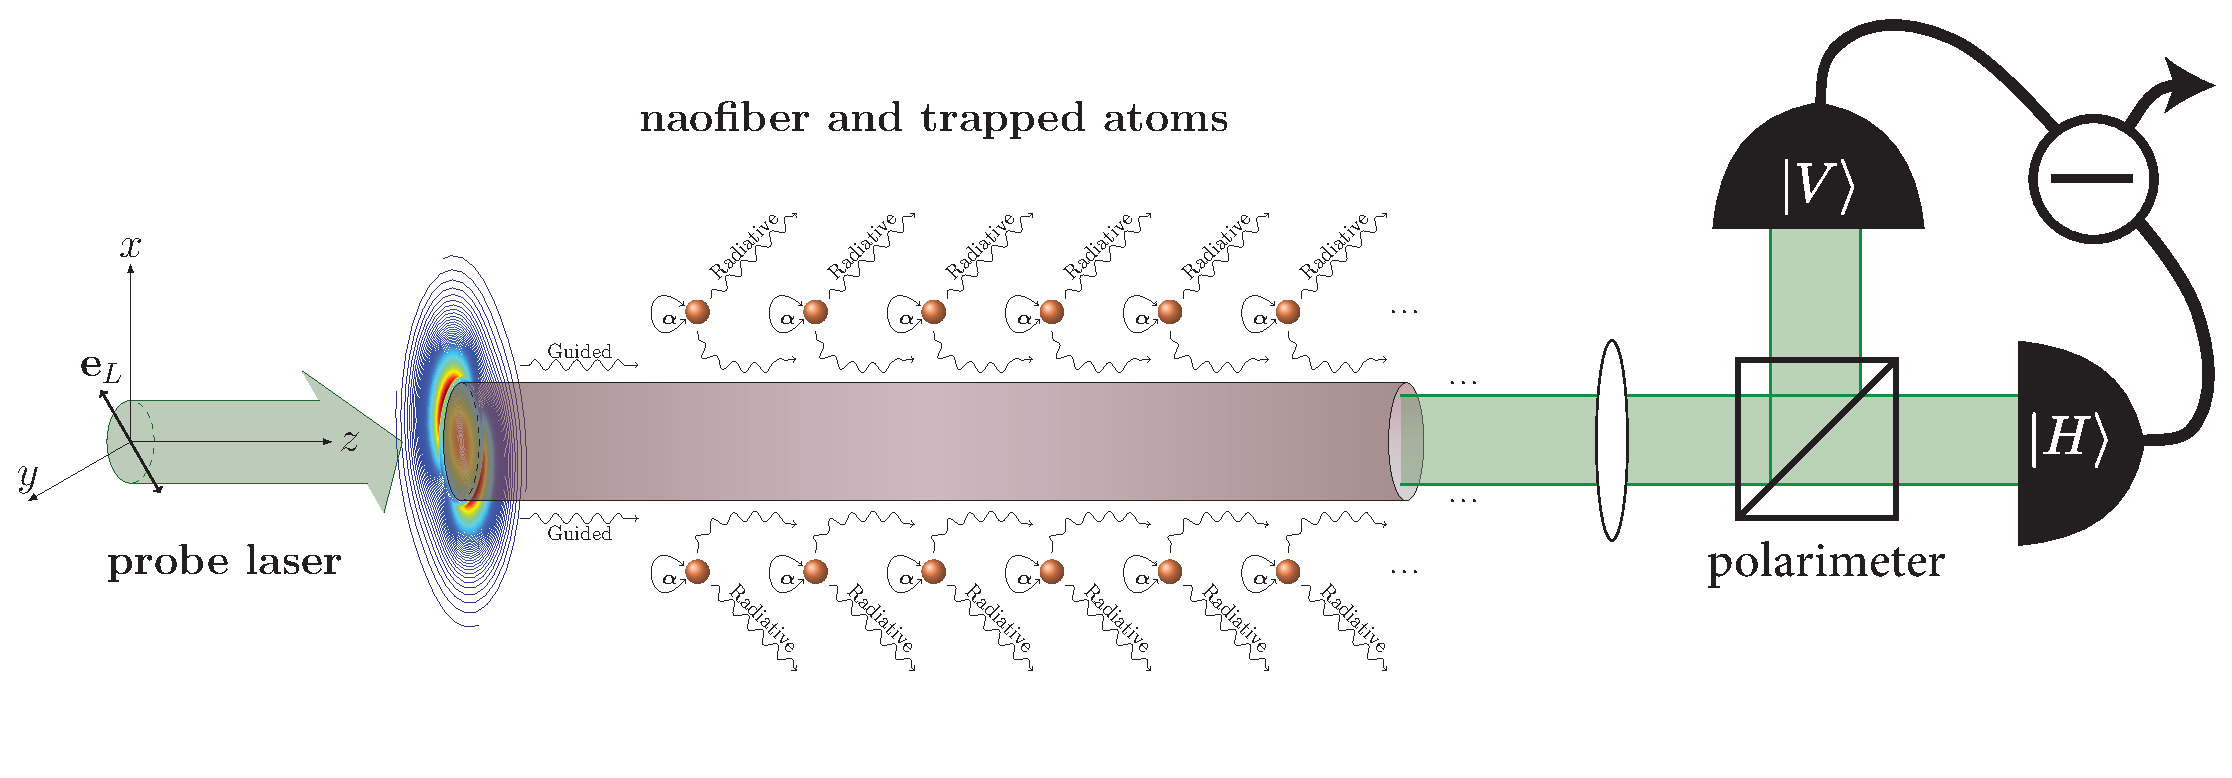
\includegraphics[width=12cm]{../media/Figs/BirefringenceMeasurement}}
\caption{Setup diagram for birefringence measurement.}
\end{figure}



\bigskip
\textbf{Comparison to the vacuum case:}

Notice that, the phase shift for an atom in vacuum can be given in a similar form by
\begin{align}
\delta\phi^{vac} &= 2\pi \frac{\omega_0}{cA} \Re[\alpha] |\mathbf{u}_{00}(\br')|^2 =  2\pi \frac{\omega_0}{c A^{vac'}_{e\!f\!f}} \Re[\alpha]=-\frac{1}{A} \sigma_0 |\mathbf{u}_{00} (r'_{\!\perp})|^2 \frac{\Gamma_{vac}}{4\Delta},
\end{align}
where $\mathbf{u}_{00}(\br')  $ is the TEM00 mode of a Gaussian laser field at the atom position, $ A=\frac{\pi W_0^2}{2} $ is the mode area of the Gaussian beam with wist $ W_0 $. Hence, the relative strength of phase shift due to the presence of a nanofiber versus vacuum can be given by
\begin{align}
\frac{\delta\phi^{nano}}{\delta\phi^{vac}} &=\frac{A_{e\!f\!f}^{vac'}}{A_{e\!f\!f}^{11}}= \frac{A}{2} \!n_g\! \frac{|\mathbf{u}_1(r_\perp^{nano'})|^2}{|\mathbf{u}_{00}(r_\perp^{vac'})|^2}.
\end{align}
In the vacuum case, the strongest mode is given by $ |\mathbf{u}_{00}(r_\perp^{vac'})|=1 $ when the atom is placed at the center of the beam waist. 



\section{Modification of the spontaneous emission of atoms trapped near a nanophotonic waveguide}


\subsection{Dipole oscillation and emission of polarized light}
Here we present some results of electrical dipole radiations.

In the Green's function language, we can obtain the electrical field emitted by an electric dipole source by
\begin{align}\label{EGd}
\mathbf{E}(\br) &=  \int\mathbf{G}(\br,\br')\cdot \mathbf{d}(\br') \mathrm{d}\br', 
\end{align}
where $ \mathbf{G}(\br,\br') $ is the dyadic Green's functions for a dipole located at $ \br' $ with a dipole moment of $ \mathbf{d}(\br') $. $\mathbf{G}(\br,\br')$ can be determined from the scalar Green's function $G_0(\br,\br')$ by 
\begin{align}
\mathbf{G}(\br,\br') = \left[\mathbbm{1} + \frac{1}{k^2}\nabla\nabla \right]G_0(\br,\br')
\end{align}
with the scalar Green's function we got in the last section given by
\begin{align}\label{scalarG}
G_0(\br,\br') = k^2\frac{e^{ik|\br-\br'|}}{|\br-\br'|}. 
\end{align}

For a discrete dipole source with $ \mathbf{d}(\br)= \mathbf{d}\delta(\br-\br') = \mathbf{d}(\br')  $, the electrical field at an arbitrary position $\br$ can be given by
\begin{align}
 \mathbf{E}(\br) &= \mathbf{G}(\br,\br')\cdot \mathbf{d}(\br'), 
\end{align}
where Gaussian units have been applied. This equation describes how a dipole emits electromagnetic wave and how the electromagnetic field distributes in space due to the oscillation of the electrical dipole source. 

In a classical picture, if there is a field $ \mathbf{E}_0 $ propagates cross the dipole source, the dipole will respond and generate a scattered field which overlaps with the incident field to yield a total field described by
\begin{align}
\mathbf{E}(\br) &= \mathbf{E}_0(\br)+\mathbf{G}(\br,\br')\cdot \mathbf{d}(\br')\\
&=\mathbf{E}_0(\br)+ \mathbf{G}(\br,\br')\cdot \tensor{\boldsymbol{\alpha}}\cdot \mathbf{E}(\br'),
\end{align}
where $ \tensor{\boldsymbol{\alpha}} $ is the atomic polarizability and $ k=\omega/c $. Under the Born approximation, the total field can be given by
\begin{align}
\mathbf{E}(\br) 
&=\mathbf{E}_0(\br)+ \mathbf{G}(\br,\br')\cdot \tensor{\boldsymbol{\alpha}}\cdot \mathbf{E}_0(\br').\label{eq:EoutG}
\end{align}

In the context of nanophotonic waveguides and atomic system, the dyadic Green's function can be written as
\begin{align}
\mathbf{G}(\br,\br') = \left\{ 
\begin{array}{lc}
\mathbf{G}_0(\br,\br')+\mathbf{G}_R(\br,\br'), & \br \, \text{ is outside of the waveguide}\\
\mathbf{G}_T(\br,\br'), & \br \, \text{ is inside of the waveguide}
\end{array}\right.,
\end{align}
where the subscript $ 0,\,R\,\text{and}\,T $ denote free-space, reflective and transmission contributions, which be can be decomposed by solving corresponding boundary value problems (will discuss in details later).
 
The atomic polarizability can be calculated through emission response models. For now, we only look at a very simple scalar response case where the polarizability tensor becomes a scalar quantity. A self-consistent equation for an atom at $ \br' $ excited by an incident electrical field can be given by 
\begin{align}
(-\omega^2+\omega_0^2)\br' &= -\frac{e}{m}\mathbf{E}(\br')\\
&=-\frac{e}{m}\left[\mathbf{E}_0(\br')+ {\alpha}\mathbf{G}(\br',\br')\cdot  \mathbf{E}(\br') \right],
\end{align}
where $\omega_0$ is the atomic resonance. Using the definitions that 
\begin{align}
\mathbf{d}(\br') &=-e\br'=\alpha \mathbf{E}(\br')\approx \alpha \mathbf{E}_0(\br'),\\
\Delta &=\omega-\omega_0,
\end{align}
and only consider the near-resonance case, we can obtain
\begin{align}
\left(-\Delta\mathbbm{1} -\frac{e^2}{2m\omega_0}\mathbf{G}(\br',\br') \right) &\cdot \mathbf{d}(\br') = \frac{e^2}{2m\omega_0}\mathbf{E}_0(\br')\\
\Rightarrow\qquad d &=\frac{\frac{e^2}{2m\omega_0}}{-\Delta-\frac{ e^2}{2m\omega_0}\hat{d}\cdot\mathbf{G}(\br',\br')\cdot \hat{d}}E_0(\br')\\
&=\frac{\frac{e^2}{2m\omega_0}}{-(\Delta+\delta \Delta)-\frac{i}{2}\Gamma}E_0(\br'),
\end{align}
where we have defined the Lamb shift $ \delta \Delta= \frac{e^2}{2m\omega_0}\re\left[\hat{d}^\dagger\cdot\mathbf{G}(\br',\br')\cdot \hat{d} \right]$ with the dipole direction $ \hat{d} $ and the radiation reaction decay rate 
\begin{align}
\Gamma &= \frac{e^2}{m\omega_0}\im\left[\hat{d}^\dagger\cdot\mathbf{G}(\br',\br')\cdot \hat{d}\right]\\
&= \Gamma_0 + \delta \Gamma,
\end{align}
with the natural linewidth $ \Gamma_0=\frac{e^2}{m\omega_0}\im\left[\hat{d}^\dagger\cdot\mathbf{G}_0(\br',\br')\cdot \hat{d}\right] $ and the shift in decay rate $ \delta\Gamma=\frac{e^2}{m\omega_0}\im\left[\hat{d}^\dagger\cdot\mathbf{G}_R(\br',\br')\cdot \hat{d}\right] $. The scripts $ \Re $ and $ \Im $ correspond to extracting real and imaginary parts operations. The scalar $ E_0(\br') $ is the projection of the incident field at $ \br' $ onto the dipole oscillating direction. Therefore, the scalar atomic polarizability can be given by
\begin{align}
\alpha &= \frac{\frac{e^2}{2m\omega_0}}{-(\Delta+\delta \Delta)-\frac{i}{2}\Gamma},
\end{align}
which includes the modification from the incident field. 

By solving the free-space dipole radiation problem, the imaginary part of the free-space Green's function can be given by
\begin{align}
\mathrm{Im}\left[ \mathbf{G}^{(0)} (\br^\prime\!_\perp, \br^\prime\!_\perp) \right] &= \mathrm{Im} 
\left[ \mathbf{G}^{rad}_{(0)}(\br'\!_\perp,\br'\!_\perp)\right]  = \frac{ 
2k^3}{3}\eye = \frac{2}{3}\left(\frac{ 
\omega}{c}\right)^3\eye
%\Im\left[\mathbf{G}_0(\br',\br') \right] =\frac{k^3}{6\pi} \mathbbm{1} \approx \frac{1}{6\pi}k^3_0\mathbbm{1}.
\end{align}
Hence the natural linewidth of an atom can be given by
\begin{align}
\Gamma_0 = \frac{2}{3}\frac{e^2\omega_0^2}{mc^3}=\frac{2}{3}k_0r_{class},
\end{align}
where $ k_0=\omega_0/c $, and $ r_{class}= \frac{e^2\omega_0}{mc^2}$ is the classical radius of the atom. After considering quantum effects, there will be a factor $ f=\frac{2m\omega_0}{\hbar e^2}|d_{eg}|^2 $ modification to the decay rates. 

\textcolor{red}{To be continued: total dipole momentum and vacuum dipole momentum, more details on quantum model for the polarizability...}
\begin{align}
\boldsymbol{\alpha} &= \sum_e \frac{\mathbf{d}_{ge}\mathbf{d}_{eg}}{-\hbar(\Delta+i\gamma_{eg}/2)}
\end{align}
The irreducible tensor decomposition can be found in the spin control and measurement long paper\cite{Deutsch2010a} or in Le Kien's dynamical polarizability of atoms paper~\cite{LeKien2013}. 


%\section{Polarizability of alkali atoms}
\subsection{Polarizability of alkali atoms}
Above, the theory we derived has not considered the real atom multilevel structure. Below, we will quantize the field and consider the inner structure of the Cs atoms.

In the interaction picture, the dipole operator associated with an atomic level $ g $ can be given by
\begin{align}\label{eq:dtop}
\hat{\mathbf{d}}(t) &= \sum_e \left[ \hat{\mathbf{d}}_{eg}e^{i(\omega_{eg}+i\gamma_{eg}/2)t} + \hat{\mathbf{d}}_{ge}e^{-i(\omega_{eg}-i\gamma_{eg}/2)t}\right]
\end{align}
where the upward and downward transitions are described by
\begin{align}
\hat{\mathbf{d}}_{eg} &= \mathbbmss{P}_e\mathbf{d}_{eg}\mathbbmss{P}_g\\
&= \ketbra{e} \mathbf{d}\ketbra{g}\\
&= \bra{e} \mathbf{d}\ket{g} \ket{e}\!\!\bra{g}\\
&= \mathbf{d}_{eg} \sigma_{eg}\\
\hat{\mathbf{d}}_{ge} &=\hat{\mathbf{d}}_{eg}^\dagger \\
&= \bra{g} \mathbf{d}^*\ket{e} \ket{g}\!\!\bra{e}\\
&= \mathbf{d}_{ge}\sigma_{ge}.
\end{align}
We denote the dipole vector $ \mathbf{d}=d\mathbf{e}_d=\sum_{q=0,\pm 1} (-1)^qd^{(q)}\mathbf{e}^*_{-q}=\sum_{q=0,\pm 1} d^{(q)}\mathbf{e}^*_{q} $ in terms of the spherical tensor components $ d^1=(d_{r\!_\perp}-id_{\phi})/\sqrt{2} $, $ d^0=d_z $ and $ d^{(-1)} =-(d_{r\!_\perp}+id_{\phi})/\sqrt{2} $, and the spherical vector basis $ \mathbf{e}_1=-((\mathbf{e}_{r\!_\perp}-i\mathbf{e}_{\phi})/\sqrt{2}) $, $ \mathbf{e}_0=\mathbf{e}_z $ and $ \mathbf{e}_{-1}=((\mathbf{e}_{r\!_\perp}+i\mathbf{e}_{\phi})/\sqrt{2}) $. The $ q $ spherical component of the dipole moment for the transition between $ e_{m'} $ and $ g_m $, for example, can be given by
\begin{align}
d^{(q)}_{e_{m'}g_{m}}&= \sum_m \langle e||d||g\rangle \bra{e,m'}g,m,1,q\rangle .
\end{align}
In the frequency domain, we define 
\begin{align}
\hat{\mathbf{d}}(\omega) &= \int_0^\infty \hat{\mathbf{d}}(t)e^{-i\omega t}\mathrm{d}t\\
&= \sum_e \left[ \frac{i\hat{\mathbf{d}}_{eg}}{ \omega -\omega_{eg}-i\gamma_{eg}/2 } + \frac{i\hat{\mathbf{d}}_{ge}}{ - \omega-\omega_{eg}-i\gamma_{eg}/2}\right].
\end{align}

Now, consider a radiation reaction that an atom is polarized in response to a traveling guided mode electric field operator $ \hat{\mathbf{E}}_0(t)=\frac{1}{2}\left[\hat{\mathbf{E}}^{(+)}_0e^{-i\omega t} +  \hat{\mathbf{E}}^{(-)}_0e^{i\omega t}\right] $, with the guided mode labeled by an index $ \mu = (\omega,f,p)$
\begin{align}
\hat{\mathbf{E}}^{(+)}_0 &= \sqrt{\frac{\hbar \omega}{v_g}} \hat{a}_\mu \mathbf{u}_{\mu} (r\!_\perp) e^{if\beta z+ip\phi},
\end{align} 
where $ \mathbf{u}_{\mu} (r\!_\perp)=\mathbf{u}_\mu(r\!_\perp,\omega) $  is one of the normalized guided modes of the nanofiber. 

The induced dipole moment can be given by
\begin{align}
\hat{\mathbf{d}}(t) 
%&= \frac{1}{2} \left[\boldsymbol{\alpha}^*(\omega)e^{i\omega t} +\boldsymbol{\alpha}(\omega)e^{-i\omega t} \right] \hat{\mathbf{E}}_0\\
&= \Re\left[ \boldsymbol{\alpha}(\omega)\hat{\mathbf{E}}_0^{(+)} e^{-i\omega t}\right]
\end{align}
with the polarizability 
\begin{align}\label{Eq::PTensorGen}
\boldsymbol{\alpha}(\omega) &=\sum_e \frac{\hat{\mathbf{d}}_{ge}\hat{\mathbf{d}}_{eg}}{\hbar(\omega_{eg} -\omega -i\gamma_{eg}/2)} =-\sum_e \frac{\hat{\mathbf{d}}_{ge}\hat{\mathbf{d}}_{eg}}{\hbar(\Delta_{eg} +i\gamma_{eg}/2)}
%\left[ \frac{1}{\omega_{eg} -\omega -i\gamma_{eg}/2 } + \frac{1}{\omega_{eg} +\omega +i\gamma_{eg}/2 } \right].
\end{align}
where we have ignored the counter-rotating terms for our near-resonance case and defined $ \Delta_{eg}=\omega-\omega_{eg} $. In the case that $ |\Delta_{eg} |\gg \gamma_{eg} $, we can ignore the $ i\gamma_{eg} $ component and simplify the polarizability of the atom as
\begin{align}
\boldsymbol{\alpha} &= -\sum_e \frac{\hat{\mathbf{d}}_{ge}\hat{\mathbf{d}}_{eg}}{\hbar\Delta_{eg}} 
\end{align} 

For a real Cesium atom case, we focus on the transition from $ F=3 $ and $ F=4 $ manifolds of the ground state $ 6S_{1/2} $ to the $ F'=3 $ manifold of the exited state $ 6P_{1/2} $. We define the dipole operator of transition from the hyperfine ground state $ f $ to the excited state $ f' $ as~\cite{Baragiola2014a}
\begin{align}
\hat{\mathbf{d}}_{f'f} &=  \sum_q \sum_{m, m'}  \bra{f' m'} d_{f'\!,f}^q \ket{f m} \op{f' m'}{f m} \mathbf{e}_q^* \\
& = \bra{ f' }| d | \ket{ f } \sum_q \sum_{m, m'}  \bravket{f m; 1 q}{f' m'} \op{f' m'}{f m} \mathbf{e}_q^*
\end{align}
where we used the Wigner-Eckart theorem to pull out the reduced matrix element $\bra{ f' }| d | \ket{ f } $.  It can be further simplified with another application of the Wigner-Eckart theorem,
	\begin{align}
		\bra{ f' }| d | \ket{ f } = \bra{ j' }| d | \ket{ j } o^{j' f'}_{j f},
	\end{align}
in terms of a reduced matrix element involving the $j \rightarrow j'$ transitions with the total nuclear angular moment quantum number $ i $ and a relative oscillator strength,
	\begin{align} \label{Eq::OscStrength}
		o^{j' f'}_{j f} \equiv (-1)^{f'+i + j' + 1} \sqrt{ (2 j'+1) (2f + 1) } 
			\left\{ 
				\begin{array}{ccc}
					f' & i & j' \\
					j & 1 & f
				\end{array}
			\right\} .
	\end{align}
that determines the spontaneous decay branching ratios on allowed dipole transitions; $\Gamma_{j' f' \rightarrow j f} / \Gamma_{j'\rightarrow j} = |o^{j' f'}_{j f}|^2$ \cite{Deutsch2010a}.	
	
This allows us to factor out characteristic units from the dipole operator and define dimensionless dipole operators,
	\begin{align}
		\hat{ \mathbf{D}}_{f' f} & = \frac{ \hat{ \mathbf{d} }_{f' f} }{\bra{ j' }| d | \ket{ j } } \\
		& = \sum_q \sum_{m, m'} \mathbf{e}_q^* o^{j' f'}_{j f} \bravket{f' m'}{f m; 1 q} \op{f' m'}{f m}. 
	\end{align}
Finally, we write the detuning from a particular hyperfine transition as
	\begin{align}
		\Delta_{f,f'} = \Delta + \delta_{f'},
	\end{align}
where we have factored out the detuning relative to the largest hyperfine excited state under $ j' $ splittings,
	\begin{align} \label{Eq::DetuningChoice}
		\Delta \equiv \Delta_{f,f'_{\rm max}} = \omega - ( \omega_{f'_{\rm max}} - \omega_f),
	\end{align} 
and $\delta_{f f'} \equiv \Delta_{f,f'} - \Delta$ is the residual detuning for the other hyperfine excited states.  All the units are collected in a characteristic polarizability\index{polarizability!characteristic polarizability},
	\begin{align} \label{Eq::alpha0}
		\alpha_0(\Delta) & =  -\frac{|  \bra{ j' }| d | \ket{ j } |^2}{\hbar \Delta } = - \frac{3 \lambda_{j' j}^3}{32 \pi^3} \frac{ \Gamma }{ \Delta }.
	\end{align}
\textcolor{red}{Note that this polarizability formula does not hold if we plug in the real numbers of Cs D1-line transition data, for example. I need to check the units later, but I would prefer to use the irreducible dipole moment element representation formula for now as it appears in Steck's data sheet.} The wavelength of the transition $\lambda_{j' j}$ and spontaneous emission rate $\Gamma$ are defined with respect to the fine-structure splitting $j' \rightarrow j$; that is,
	\begin{align}
		\Gamma = \frac{1}{\hbar} \frac{4}{3} \frac{\omega_{j j'}^3}{c^3} | \bra{ j' }| d | \ket{ j } |^2.
	\end{align}
One could define a slightly different characteristic polarizability using a different detuning in \erf{Eq::DetuningChoice}, such as the fine structure splitting on the $j \rightarrow j'$ transition.

The atomic polarizability tensor in \erf{Eq::PTensorGen} can then be written in terms of the dimensionless dipole operators and the characteristic polarizability,
\begin{align} \label{Eq::AtomicPolarizabilityF}
\tensor{\boldsymbol{\alpha}}(f) &=  \alpha_0(\Delta) \sum_{f'} \frac{ \hat{\mathbf{D}}_{f f'} \hat{\mathbf{D}}_{f' f}}{ 1 + \delta_{f'} / \Delta + i \Gamma/(2\Delta)}\\
& = \alpha_0(\Delta) \sum_{q,q'}  \sum_{f,f'} \sum_{m_1, m_2, m'}  \frac{\mathbf{e}_q \mathbf{e}^*_{q'} | o^{j'f'}_{jf} |^2 C^{fm_2;1q}_{f'm'} C^{fm_1;1q'}_{f'm'} \op{f m_2}{f m_1}}{1 + \delta_{f'} / \Delta + i \Gamma/(2\Delta)},
\end{align}
where $ C^{fm;1q}_{f'm'}=  \bravket{f' m'}{f m; 1 q}= \bravket{f m; 1 q}{f' m'}$ is the Clebsch-Gordan coefficient. Also nothing that $m' = m_1 + q'$ and $m' = m_2 + q$ and thus
\begin{align}
	m_2 - m_1 = q-q'.
\end{align}

For ${}^{133}$Cs with ground hyperfine manifolds $f = \{3,4\}$, this gives
\begin{align}
\tensor{\boldsymbol{\alpha}}(3) 
		& = \alpha_0(\Delta_{3}) \sum_{f'} \frac{ \hat{\mathbf{D}}_{3 f'} \hat{\mathbf{D}}_{f' 3}}{ 1 + \delta_{3, f'} / \Delta_{3} + i \Gamma/(2\Delta_3) } \\
		&= \alpha_0(\Delta_{3}) \sum_{f'} \sum_{q,q'} \sum_{m_1, m_2, m'}\frac{ \mathbf{e}_q \mathbf{e}^*_{q'} | o^{j'f'}_{j3} |^2 C^{3m_2;1q}_{f'm'} C^{3m_1;1q'}_{f'm'} \op{3 m_2}{3 m_1}}{ 1 + \delta_{3, f'} / \Delta_{3} + i \Gamma/(2\Delta_3) }\\
\tensor{\boldsymbol{\alpha}}(4) &=\alpha_0(\Delta_{4}) \sum_{f'} \frac{ \hat{\mathbf{D}}_{4 f'} \hat{\mathbf{D}}_{f' 4}}{ 1 + \delta_{4, f'} / \Delta_{4} + i \Gamma/(2\Delta_4) }\\
	 &= \alpha_0(\Delta_{4}) \sum_{f'} \sum_{q,q'} \sum_{m_1, m_2, m'}\frac{ \mathbf{e}_q \mathbf{e}^*_{q'} | o^{j'f'}_{j4} |^2 C^{4m_2;1q}_{f'm'} C^{4m_1;1q'}_{f'm'} \op{4 m_2}{4 m_1}}{ 1 + \delta_{4, f'} / \Delta_{4} + i \Gamma/(2\Delta_4)} .
\end{align}
We have explicitly labeled the detunings by the ground state hyperfine level $f$ in order to emphasize that the detunings are different on each of the two terms.  Unless the laser detuning is chosen such that $\Delta_3$ and $\Delta_4$ are of the same order, one of the two terms will dominant the dynamics and the other can be ignored.


% Irreducible tensors.
\subsection{Irreducible tensor representation of atomic polarizability}
\textcolor{red}{Content around this part is mainly copied from Ben's dissertation with some modifications.}
The atomic polarizability tensor, being a dyad of two vector operators, can be decomposed into rank-0, rank-1, and rank-2 irreducible tensor components \cite{Stockton2007, Hammerer2006, Geremia2006, Deutsch2010a, LeKien2013}.  The terms in the Hamiltonian can be written in a Cylindrical basis, $ (r\!_\perp,\phi,z) $, which is useful for describing atomic interaction with nanofiber field. The dimensionless Cylindrical $ij$-component of the atomic polarizability tensor\index{polarizability!polarizability tensor} in the ground hyperfine state $f$ is defined,
\begin{align} \label{Eq::alphaij}
\hat{\alpha}_{ij}(f) &\equiv \mathbf{e}_i \cdot \hat{\mathbf{D}}_{f f'} \hat{\mathbf{D}}_{f' f} \cdot \mathbf{e}_j\\
&= \sum_{q,q'} \sum_{m_1, m_2, m'} \mathbf{e}_i \cdot\mathbf{e}_q \mathbf{e}^*_{q'}\cdot \mathbf{e}_j | o^{j'f'}_{jf} |^2 C^{fm_2;1q}_{f'm'} C^{fm_1;1q'}_{f'm'} \op{f m_2}{f m_1}.
\end{align}	
It can be shown that the block-diagonal terms have a basis-independent form whose Cartesian $ij$-components are \cite{Deutsch2010a},
	\begin{align} \label{Eq::IrreducibleDecomp}
		\hat{\alpha}_{ij} (f) = C_{j' f f'}^{(0)} \delta_{ij} \hat{ I } + i C_{j' f f'}^{(1)} \varepsilon_{ijk} \hat{f}_k + C_{j' f f'}^{(2)} \left(\frac{1}{2} \big(\hat{f}_i \hat{f}_j + \hat{f}_j \hat{f}_i \big) - \frac{1}{3} \delta_{ij} \hat{ \mathbf{f} } \cdot \hat{ \mathbf{f} }  \right).  
	\end{align}
The $\hat{f}_i$ are dimensionless hyperfine spin operators satisfying
	\begin{align}
		[\hat{f}_i, \hat{f}_j] = i \varepsilon_{ijk} \hat{f}_k,
	\end{align}
with total angular momentum $f$ for each ground hyperfine manifold.  The tensor coefficients are~\cite{Deutsch2010a}
		\begin{align}
			C_{j' f f'}^{(0)} &= (-1)^{3f - f' + 1} \frac{1}{ \sqrt{3} } \frac{2f'+1}{\sqrt{2f+1}}  \left\{ \begin{array}{ccc} f& 1 & f' \\ 1 & f & 0 \end{array} \right\} |o^{j' f'}_{j f}|^2, \\
			C_{j' f f'}^{(1)} &= (-1)^{3f - f' } \sqrt{\frac{3}{ 2} } \frac{2f'+1}{ \sqrt{f(f+1)(2f+1)} }  \left\{ \begin{array}{ccc} f & 1 & f' \\ 1 & f & 1 \end{array} \right\} |o^{j' f'}_{j f}|^2, \\
			C_{j' f f'}^{(2)} &= (-1)^{3f - f' } \frac{\sqrt{30} (2f'+1)}{\sqrt{ f(f+1)(2f+1)(2f-1)(2f+3))} }  \left\{ \begin{array}{ccc} f & 1 & f' \\ 1 & f & 2 \end{array} \right\} |o^{j' f'}_{j f}|^2 .
		\end{align}	
These coefficients depend on the fine-structure quantum numbers $\{j, j'\}$ through the relative oscillator strengths, $o^{j' f'}_{j f}$, given in \erf{Eq::OscStrength}.  Note that the notation in \erf{Eq::alphaij} is different from that for the full polarizability tensor, \erf{Eq::AtomicPolarizabilityF}, (and different from that in Ref. \cite{Deutsch2010a}) in that it contains no units, detunings, or sums over excited states.  Instead its intention is to isolate the irreducible tensor components.   

When the detuning is very large compared to the excited hyperfine splitting the detuning becomes independent of $f'$ (essentially $\delta_{f'}/\Delta \rightarrow 0$).  Then, the sums over the tensor coefficients in Eqs. (\ref{Eq::GenPolarizability}) can be done explicitly to yield,
	\begin{align}
		C_{j' f}^{(0)} &\equiv \sum_{f'} C_{j' f f'}^{(0)} =   \frac{2^{j'-1/2}}{3} \label{Eq::ScalarCoefSum} \\ 
		C_{j' f}^{(1)} &\equiv  \sum_{f'} C_{j' f f'}^{(1)} = (-1)^{j'-1/2} \frac{g_f}{3} \\
		C_{j' f}^{(2)} &\equiv  \sum_{f'} C_{j' f f'}^{(2)} = 0. \label{Eq::Rank2Sum}
	\end{align}
The Land\'{e} g-factor depends on the ground state manifold:  $g_f = 1/f_{\uparrow}$ for $f_{\uparrow} = i + 1/2$ and $g_f = -1/f_{\uparrow}$ for $f_{\downarrow} = i - 1/2$.  In this far-detuned limit, we see that the $C_{j' f f'}^{(2)}$ coefficients sum to zero and the rank-2 terms in \erf{Eq::GenPolarizability} vanish,
	\begin{equation} \label{Eq::GenPolarizability}
		\hat{\alpha}_{ij} (f) \rightarrow  C_{j' f}^{(0)} \delta_{ij} \hat{ I } + i C_{j' f }^{(1)} \varepsilon_{ijk} \hat{f}_k  .
	\end{equation}
This reflects the fact that in the absence of hyperfine resolution, the nuclear spin is decoupled and the ground state angular momentum is given by the total electronic angular moment, $j=1/2$. 


\subsection{Modification of decay rates of atomic transitions}
\qxd{To be moved from the FaradayProtocol notes.}

\begin{figure}[!htb]
  \centering
  \begin{minipage}[h]{\linewidth}
  %\begin{tabular}{*{2}{b{0.2\textwidth-2\tabcolsep}}}
  \hspace{-30pt}
   \subfloat[h][$ \Gamma_{\rm nanofiber}/\Gamma_0 $]{
     \includegraphics[width=0.5\textwidth]{../media/Figs/nanofiber_decayrates.tex}
     %\includegraphics[width=0.5\textwidth]{../media/Figs/FaradayProtocol-Figure14}
     \label{fig:nanofiber_decayrates}
     }
    \hfill
   \subfloat[h][$\Gamma_{\rm SWG}/\Gamma_0$]{
     \includegraphics[width=0.51\textwidth]{../media/Figs/swg_decayrates.tex}
     %\includegraphics[width=0.51\textwidth]{../media/Figs/FaradayProtocol-Figure15}
     \label{fig:swg_decayrates}
     }
    \end{minipage}
    %\end{tabular}
\caption{Polarization-dependent decay rates for the nanofiber \protect\subref*{fig:nanofiber_decayrates} and SWG \protect\subref*{fig:swg_decayrates} as functions of the radial distance to the waveguides' symmetric centers. Line types differ the contributions from the guided and radiative modes and the combined total value; colors distinguish the polarizations of $ \sigma_\pm $, $ \pi $ and the averaged case. }\label{fig:decayrates}
\end{figure}

\section{Geometric effects of dielectric waveguide interfaces}
\subsection{Modified decay rates in the perspective of waveguide geometry}

\begin{align}
\Gamma_{vac} &= \frac{4\omega_0^3|\mathbf{d}|^2}{3\hbar c^3}=-\frac{8\pi \omega_0^2}{\hbar c^2}\left[ \mathbf{d}\cdot \mathrm{Im}[\mathbin{\color{red}{\mathbf{G}^{(0)}}}(\br',\br')]\cdot \mathbf{d}^* \right]\\
\Gamma &= -\frac{8\pi \omega_0^2}{\hbar c^2}\left[ \mathbf{d}\cdot \mathrm{Im}[\mathbf{G}(\br',\br')]\cdot \mathbf{d}^* \right]\\
&=-\frac{8\pi \omega_0^2}{\hbar c^2}\left[ \mathbf{d}\cdot \mathrm{Im}[\mathbin{\color{red}{\mathbf{G}^{(0)}}}(\br',\br')+\mathbin{\color{red}{\mathbf{G}^{(R)}}}(\br'\br')]\cdot \mathbf{d}^* \right]\\
\end{align}
\begin{align}
\Gamma &\propto -\mathbf{d}\cdot \mathrm{Im}[\mathbf{G}(\br',\br')]\cdot \mathbf{d}^* \\
&=\mathrm{tr}\left[ \mathbin{\color{red}{(\mathbf{d}^*\mathbf{d})}}\cdot\mathbin{\color{blue}{ \mathrm{Im}[\mathbf{G}^*(\br',\br')]}}  \right]\\
&= \mathrm{tr}\left[ \boldsymbol{\rho} \cdot \mathrm{Im}[\mathbf{G}^{*}(\br',\br')]  \right]\ge 0
\end{align}
where $\boldsymbol{\rho}=(\mathbf{d}^*\mathbf{d})$ is defined as the dipole orientation tensor. 

Therefore, $\mathrm{Im}[\mathbf{G}^{*}(\br',\br')]$ is positive definite. 
\begin{align}
\mathrm{Im}[\mathbf{G}^{*}(\br',\br')] &= \sum_{i=1,2,3} \mathbin{\color{red}{g_i}}\hat{\mathbf{v}}_i\hat{\mathbf{v}}_i,\,\text{with}\, g_i>0.
\end{align}
$\hat{\mathbf{v}}_i$ form the principal axes of the decay rate. 
\begin{align}
\Gamma &= C(\omega)\sum_i g_i(\hat{\mathbf{v}}_i\cdot \boldsymbol{\rho}\cdot \hat{\mathbf{v}}_i) 
= \sum_i \mathbin{\color{blue}{(d'_i)^2}} \mathbin{\color{red}{g_i}} \\
&= \mathbin{\color{red}{\Gamma_1}}\cos^2\phi\sin^2\theta+\mathbin{\color{red}{\Gamma_2}}\sin^2\phi\sin^2\theta+\mathbin{\color{red}{\Gamma_3}}\cos^2\theta,
\end{align}
where $ d'_i=\sqrt{\hat{\mathbf{v}}_i\cdot \boldsymbol{\rho}\cdot \hat{\mathbf{v}}_i}$ and $\mathbf{d}'=\sum_i d'_i\hat{\mathbf{v}}_i$ defines the equivalent dipole orientation of the atomic polarizability transition.

$$\mathbin{\color{red}{\Gamma_1}}=\Gamma_{max}\mathbin{\color{red}{\ge \Gamma (\theta,\phi) \ge}} \Gamma_{min}=\mathbin{\color{red}{\Gamma_3}}$$

\begin{figure}[!tbp]
\centering\makebox[\textwidth]{
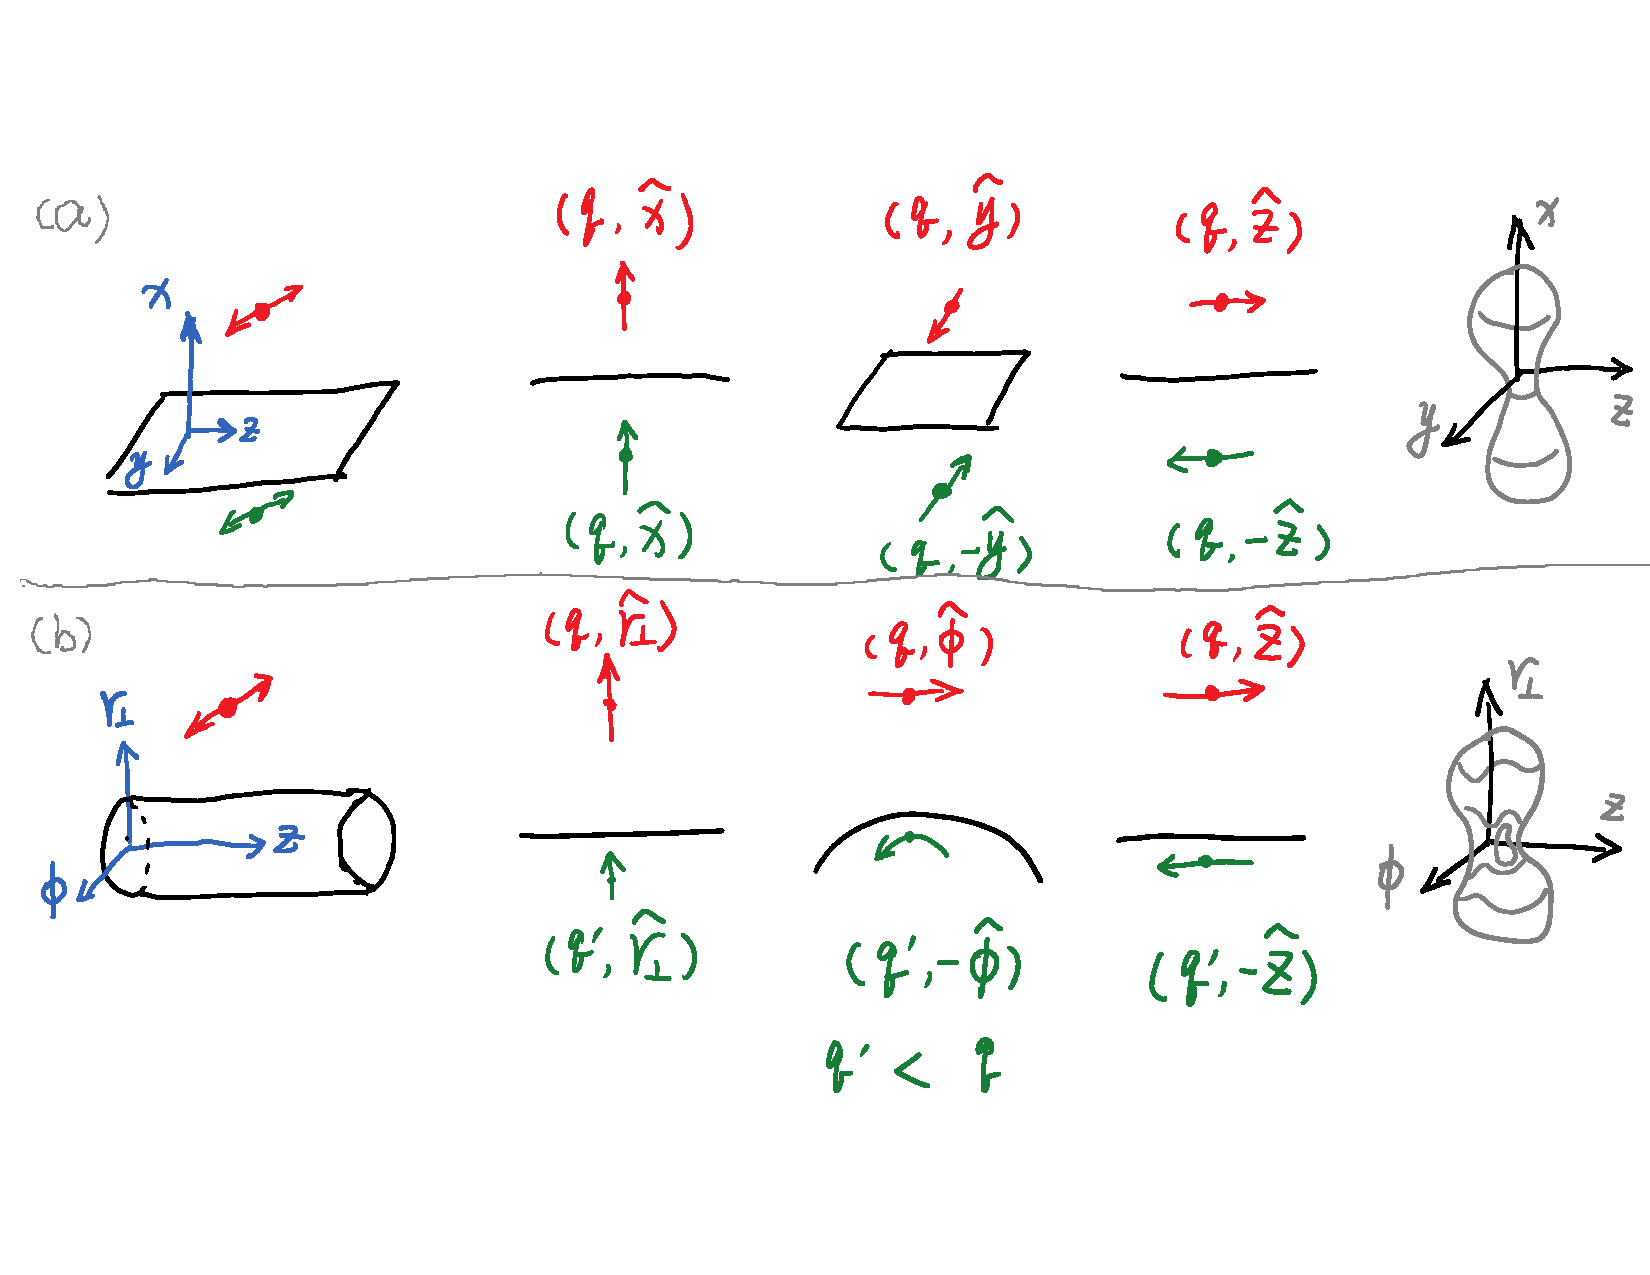
\includegraphics[width=0.8\textwidth]{../media/Figs/dipoleorientation}}
\caption{Modified dipole decay rates due to image dipoles mirrored on flat (a) and cylindrical (b) surfaces.}
\end{figure}

\begin{figure}[!tbp]
\centering\makebox[\textwidth]{
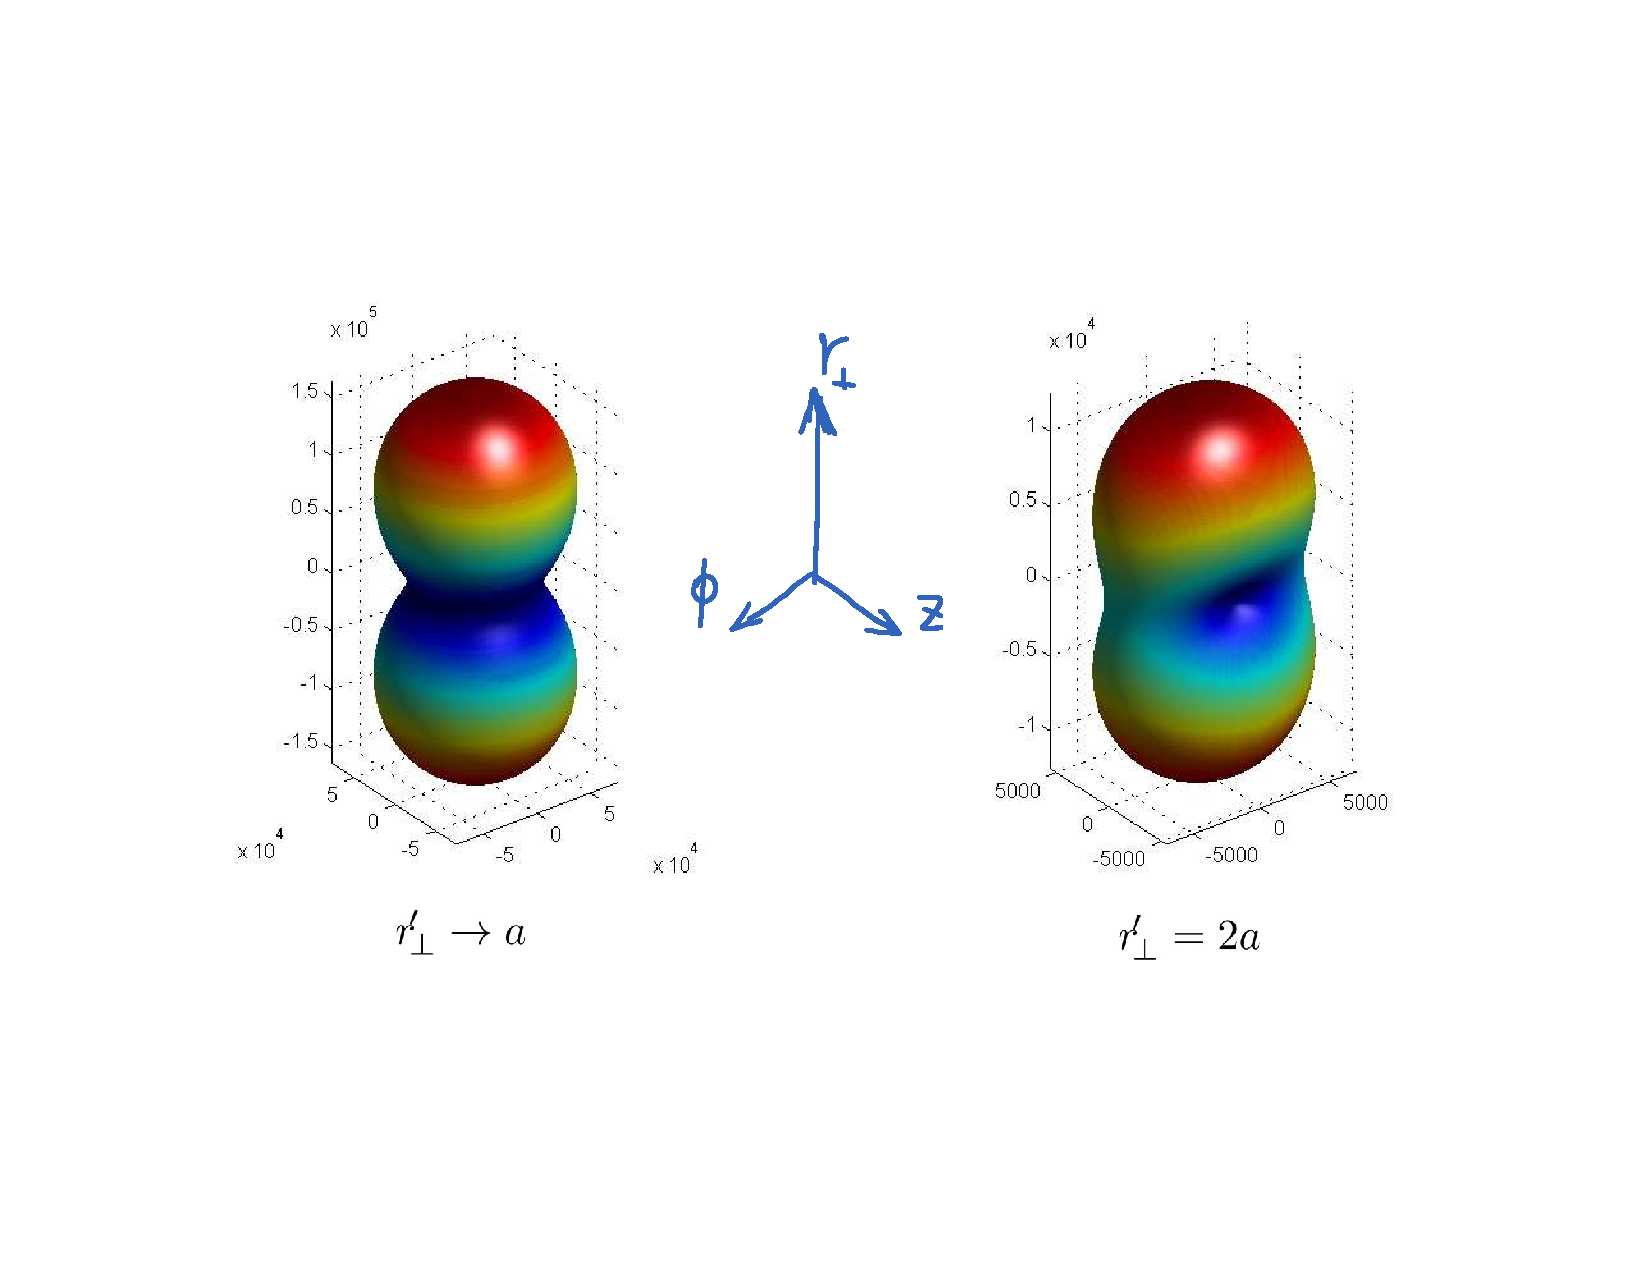
\includegraphics[width=0.8\textwidth]{../media/Figs/emissionsurfacefiber}}
\caption{Dipole emission surface in presence of a nanofiber when $ r\!_\perp=a $ (left) and $ r\!_\perp=2a $ (right).}
\end{figure}

\subsection{Enhanced anisotropy of $ H $ and $ V $ modes with different geometries of waveguides}

\begin{figure}[!tbp]
\centering\makebox[\textwidth]{
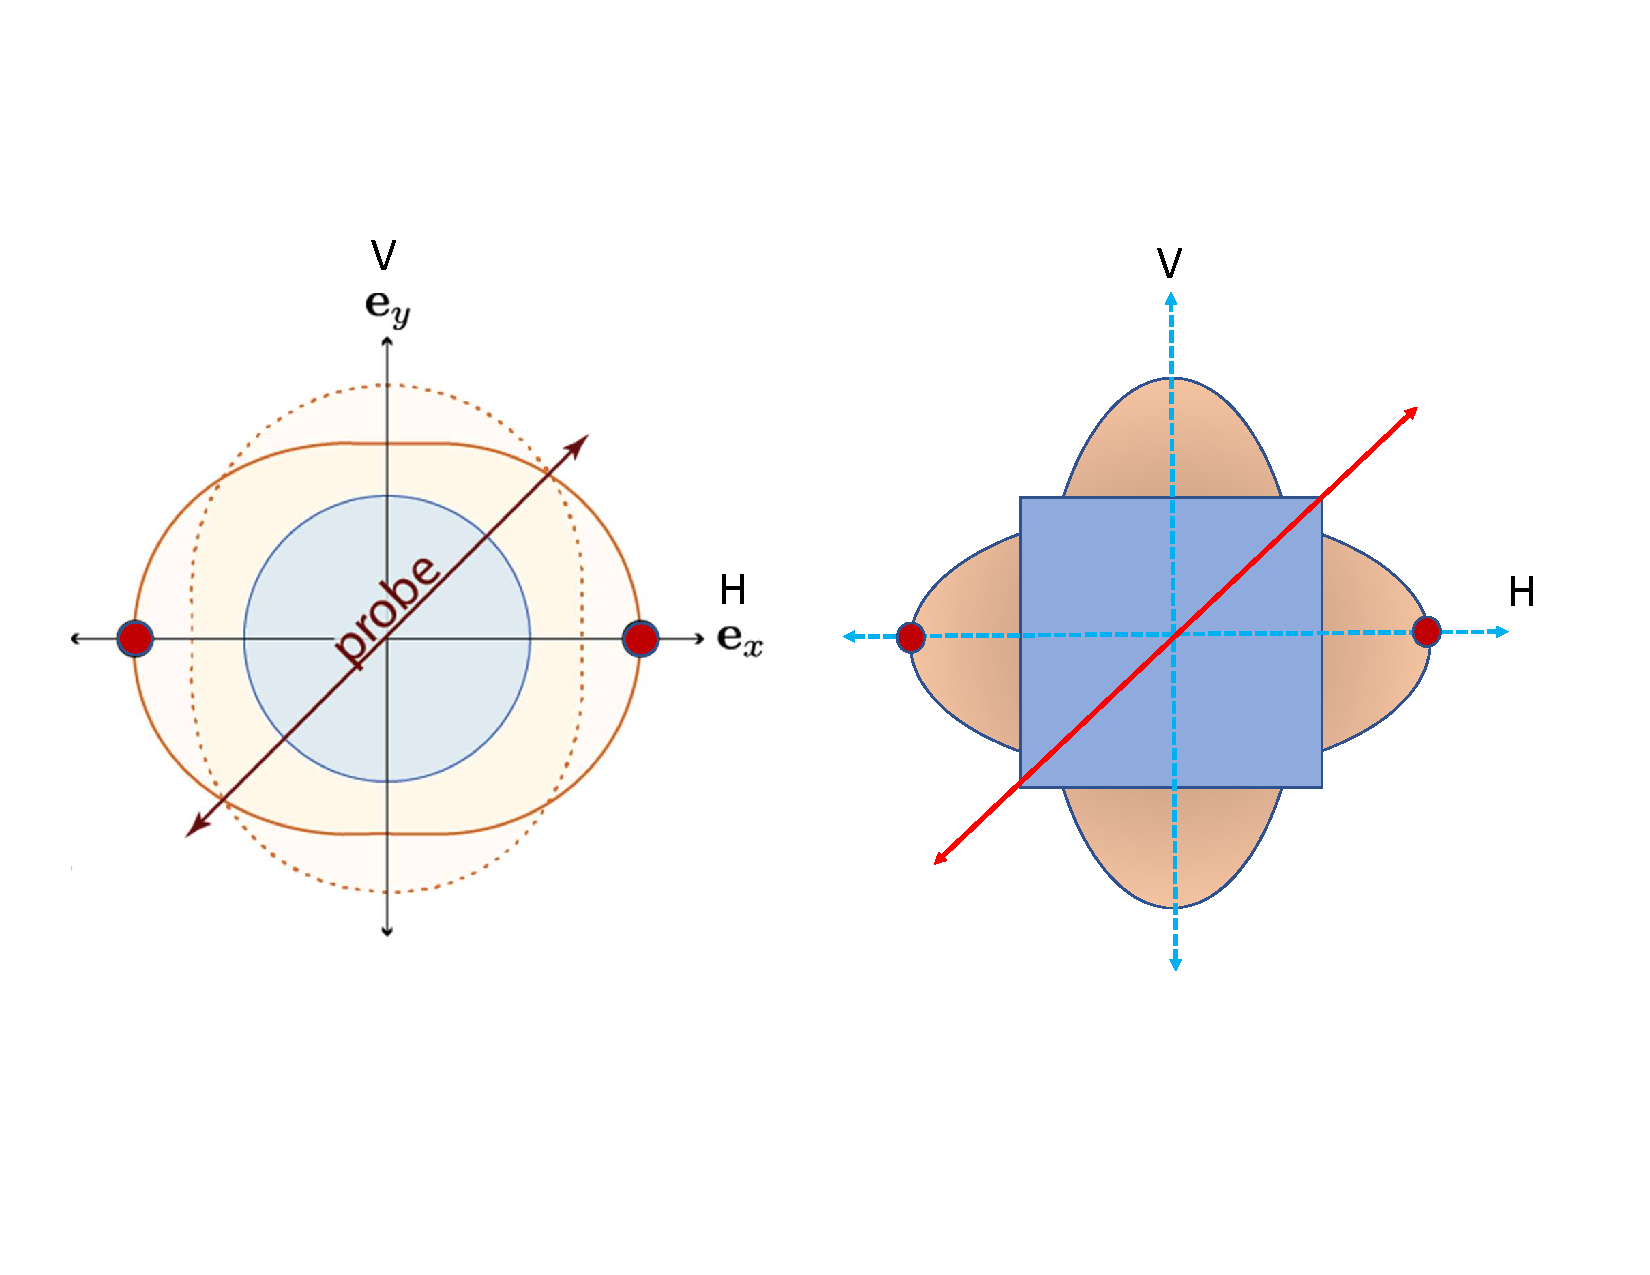
\includegraphics[width=0.8\textwidth]{../media/Figs/anisotropicmodes}}
\caption{Anisotropic guided modes of a nanofiber (left) and a \SWG (right).}
\end{figure}

%</waveguideinterface>



\appendix
% ########################### Apendix ##########################################

%<*eigenmodes>

\chapter{Fundamental eigenmodes of an optical nanofiber}\label{chap:fibereigenmodes}
In this appendix chapter, we will provide some details on solving the eigenmodes of the nanofiber starting from the homogeneous wave equation, Eq.~\ref{EBz}, and will give the formulas for mode normalization based on power and the eigenmode normalization condition. At the end of this chapter, we will also derive the formulas for calculating the group velocity of the \HE mode of the nanofiber.

First, using the relationship that
\begin{align}
\nabla^2 \!_\perp = \frac{1}{r_{\!\perp}}\pp{}{r\!_\perp}\! \left(r\!_\perp \pp{}{r\!_\perp} \right) + 
\frac{1}{r_\perp^2} \spp{}{\phi},
\end{align}
and the symmetry of the fiber,  we can separate the mode function by
\begin{align}
\psi(r\!_\perp,\phi)=\mathcal{E}_{z,\beta m}(r\!_\perp)e^{im\phi},
\end{align} 
and hence
\begin{align}
\mathcal{E}_z(r\!_\perp,\phi,z) = \mathcal{E}_{z,\beta m}(r\!_\perp)e^{i(m\phi+\beta z)},
\end{align}
where $ \mathcal{E}_{z,\beta m}(r\!_\perp) $ satisfies the Bessel's equation
\begin{align}
\left[ \spp{}{r\!_\perp}+ \frac{1}{r_{\!\perp}}\pp{}{r\!_\perp}- 
\frac{m^2}{r^2\!_\perp} + (k^2\varepsilon(r\!_\perp)-\beta^2) \right] 
\mathcal{E}_{z,\beta m}(r\!\!_\perp)=0
\end{align}
with 
\begin{align}
\varepsilon(r\!\!_\perp) = 
\begin{cases}
1, & r\!_\perp>a\\
\varepsilon_f, & r\!_\perp\leq a.
\end{cases}
\end{align}
The general solution for $ \mathcal{E}_{z,\beta m}(r\!\!_\perp) $ can be given in three cases 
corresponding to different 
boundary conditions
\begin{align}
\mathcal{E}_{z,\beta m}(r\!\!_\perp) = \begin{cases}
AJ_m(qr\!\!_\perp) + B Y_m(qr\!_\perp)&\rightarrow J_m(\theta)\sim \cos\theta,\, Y_m(\theta)\sim 
\sin\theta.\\
CI_m(qr\!_\perp) + DK_m(qr\!_\perp) & \rightarrow I_m(\theta) \sim e^\theta,\, K_m(\theta) \sim 
e^{-\theta}.\\
EH_m^{(\!1\!)}(qr\!_\perp) \!+\! FH_m^{(\!2\!)}(qr\!_\perp ) & \rightarrow H_m^{(\!1\!)} (\theta) \! \sim \! 
e^{i\theta},\, 
H_m^{(\!2\!)}(\theta)\!\sim\! e^{\!-i\theta}.
\end{cases}
\end{align}
The positive parameter $ 1/q $ is the characteristic decay length corresponding to $ 1/h_{11} $ and $ 
1/q_{11} $ 
in the $\text{HE}_{11}$ mode expression. Using the symmetric and convergent condition at $ 
r\!_\perp=0\,\text{and}\, \infty $, as for bound modes, for example, if $k< \beta\leq 
k\sqrt{\varepsilon_f}$,
\begin{align}
\left\{
 \begin{array}{lcll}
	r\!_\perp \leq a, & \mathcal{E}_{z,\beta m}(r\!_\perp )\!=\! AJ_m(h r\!_\perp), & h \!=\! 
	\sqrt{k^2\varepsilon_f-\beta^2}\! >\! 0;\\
	r\!_\perp > a, & \mathcal{E}_{z,\beta m}(r\!_\perp )\!=\!DK_m(q r\!_\perp), & q\!=\! 
	\sqrt{\beta^2-k^2}>0.
 \end{array}\right.
\end{align}
Both $ \beta $ and $ h $ are discrete for bound modes. 
For scattered modes, $ 0\leq \beta< k $, similarly, 
\begin{align}
\left\{
 \begin{array}{lcll}
	r\!_\perp \leq a, & \mathcal{E}_{z,\beta m}(r\!_\perp )\!=\! AJ_m(h r\!_\perp), & h \!=\! 
	\sqrt{k^2\varepsilon_f-\beta^2}\! >\! 0;\\
	r\!_\perp > a, & \mathcal{E}_{z,\beta m}(r\!_\perp )\!=\!EH_m^{(\!1\!)}(p r\!_\perp\!), & p\!\!=\!\! 
	\sqrt{k^2-\beta^2}>0.
 \end{array}\right.
\end{align}
Both $ \beta $ and $ p $ are continuous. 
%\textcolor{red}{(Double check the general solutions and the consistence with Eq.~\ref{ET0Rexpand}.)}
%Notice that Ref.\cite{Snyder1983} used $ J_m(hr\!_\perp)\cos m\phi $ and $ 
%(J_m(pr\!_\perp)+CH_m^{(\!1\!)})\cos m\phi $ as the basis for the general solution of $ e $ and $ o $ 
%light 
%of the radiation modes, and summed them up. They are equivalent to the solution here.  

If $ \beta $ is a pure imaginary number, the field will have an exponential decay amplitude on the $ z $ direction, and will spread the energy away from the fiber axis. Reference~\cite{Snyder1983} denotes the modes with pure imaginary $ \beta $ as evanescent modes. If $ \beta $ has both real and imaginary parts, the modes are denoted as leaky modes, which are combinations of radiation modes and evanescent modes. Except for the case that the incident light is highly directed at the complementary critical angle $ \theta_c $ of geometric optics, only the radiation modes part can propagate for a long distance along the fiber axis. In our nanofiber system, we only consider the bound and radiation modes. The ranges of some waveguide parameters are given in Table~\ref{tab:fiberparameters}. 
In the table, we have defined the normalized wave number\cite{Snyder1983Optical}, or 
$V$-number\index{$V$-number} 
of a fiber as $V  = 
k_f a \mathrm{NA}$.  Here $k_f=\frac{2\pi}{\lambda}$, is the free space wave number, $a$ is the radius 
of the core of the fiber, and $\mathrm{NA}$ is the numerical aperture\index{numerical aperture} of 
the fiber, $\mathrm{NA} = 
(n_{core}^2 - n_{cladding}^2)^{1/2} = n_{core}(2\Delta)^{1/2}$, with profile height 
parameter\index{profile height parameter} 
$\Delta =\frac{1}{2}(1-n_{cladding}^2/n_{core}^2)\approx (n_{core}-n_{cladding})/n_{core}$.  For 
different modes labeled with $ j $, we always have $V_j^2=a^2(h_j^2+q_j^2)$ and $ \lambda\beta_j/2\pi $ is a mode invariance.  The TE and TM modes have non-vanishing cut-off 
frequencies, as $ a\rightarrow 0 $.  The cutoff frequency is found from $V = a\omega (\Delta)^{1/2}/c =2.405$ for silicon fiber.  
Only the lowest HE mode, $\mathrm{HE}_{11}$, has no cutoff frequency as $ a\rightarrow 0 $.  For $0 < V < 2.405$, which is the case of the nanofiber we are studying, it is the only mode that propagates in the 
fiber. For fixed $ \varepsilon_f $, in the range that $ 0\leq \beta \leq 
k\sqrt{\varepsilon_f} $, we can distinguish the radiation and bound mode as follows:
\begin{align}
\begin{cases}
0\leq \beta < k, &\rightarrow \emph{unbounded radiation modes;}\\
k< \beta \leq k \sqrt{\varepsilon_f}, &\rightarrow \exists a,\, \emph{HE}_{11}\, \emph{is the only 
bound mode.}
\end{cases}
\end{align}


\begin{minipage}{0.97\textwidth}
\centering
\captionof{table}{Ranges of fiber parameters for different modes. } \label{tab:fiberparameters} 
\begin{tabular}{|l|c|c|c|}
\hline  & $\beta$ & $h$ & $p$ \\ 
\hline Bound modes & $k<\beta_j \leq k\sqrt{\varepsilon_f} $ & $ 0\leq h_j<V/a $ & $ p^r_j=0,\, p^i_j>0 $ \\ 
\hline Radiation modes & $0\leq \beta<k$ & $V/a < h\leq k\sqrt{\varepsilon_f}$ & $0<p\leq k $\\ 
\hline Evanescent modes & $ \beta^r=0,\, \beta^i>0 $ & $ k\sqrt{\varepsilon_f} < h $ & $ k<p $ \\ 
\hline 
\end{tabular} 
\par
\bigskip
%The caption:
Superscripts $ r $ and $ i $ denote real and imaginary parts. Subscripts $ j $ denotes the discrete indeces for bound modes. Adapted from Ref.~\cite{Snyder1983} P.P.516 Table 25-1. This can also be understood in geometric optics as shown in Fig.(\ref{fig:Fibermodes}).
\end{minipage}
\bigskip



Due to the symmetry of equations, we also have
\begin{align}
\mathcal{B}_z(r\!_\perp,\phi,z) = \mathcal{B}_{z,\beta m}(r\!_\perp)e^{i(m\phi+\beta z)},
\end{align}
where $  \mathcal{B}_{z,\beta m}(r\!_\perp) $ satisfies the same Bessel's equation as above.  

In the case of a nanofiber with a sub-wavelength radius, the high-order modes of the nanofiber can hardly be supported, which only leaves over the \HE mode\index{mode!HE11 mode@HE$_{11}$ mode} propagating along the nanofiber. Assuming the incident light is quasi-linearly polarized, the Cartesian components of the bound optical field are given, for $ r_\perp>a $ (outside the fiber), by~\cite{Lacroute2012,LeKien2004}
\begin{subequations}
\label{Ertrga}
\begin{align}
E_x^g(r_\perp,\phi,z,t) &= iA \frac{\beta_{11}J_1(h_{11}a)}{2q_{11}K_1(q_{11}a)}[(1-s_{11})K_0(q_{11}r_\perp)\cos (\varphi_0) \nonumber\\
&\qquad + (1+s_{11})K_2 (q_{11}r_\perp) \cos (2\phi-\varphi_0) ] e^{-i(\omega t-f\beta_{11}z)},\\
E_y^g(r_\perp,\phi,z,t) &= iA \frac{\beta_{11}J_1(h_{11}a)}{2q_{11}K_1(q_{11}a)}[(1-s_{11})K_0(q_{11}r_\perp)\sin (\varphi_0) \nonumber\\
&\qquad + (1+s_{11})K_2 (q_{11}r_\perp) \sin (2\phi-\varphi_0) ] e^{-i(\omega t-f\beta_{11}z)},\\
E_z^g(r_\perp,\phi,z,t) &= fA \frac{J_1(h_{11}a)}{K_1(q_{11}a)}K_1(q_{11}r_\perp)\cos (\phi-\varphi_0) e^{-i(\omega t-f\beta_{11}z)},
\end{align}
\end{subequations}
and, for $ r_\perp<a $ (inside the nanofiber), by
\begin{subequations}
\label{Ertrla}
\begin{align}
E_x^g(r_\perp,\phi,z,t) &= iA \frac{\beta_{11}}{2h_{11}}[(1-s_{11})J_0(h_{11}r_\perp)\cos (\varphi_0) \nonumber\\
&\qquad - (1+s_{11})J_2 (h_{11}r_\perp) \cos (2\phi-\varphi_0) ] e^{-i(\omega t-f\beta_{11}z)},\\
E_y^g(r_\perp,\phi,z,t) &= iA \frac{\beta_{11}}{2h_{11}}[(1-s_{11})J_0(h_{11}r_\perp)\sin (\varphi_0) \nonumber\\
&\qquad - (1+s_{11})J_2 (h_{11}r_\perp) \sin (2\phi-\varphi_0) ] e^{-i(\omega t-f\beta_{11}z)},\\
E_z^g(r_\perp,\phi,z,t) &= fA J_1(h_{11}r)\cos (\phi-\varphi_0) e^{-i(\omega t-f\beta_{11}z)},
\end{align}
\end{subequations}
with
\begin{subequations}
\begin{align}
s_{11} &= \left[\frac{1}{(h_{11}a)^2}+ \frac{1}{(q_{11}a)^2} \right] \left[ \frac{J_1'(h_{11}a)}{h_{11}aJ_1(h_{11}a)} + \frac{K'_1(q_{11}a)}{q_{11}aK_1(q_{11}a)} \right],\\
h_{11} &= \sqrt{k_0^2 n_1^2-\beta_{11}^2},\\
q_{11} &= \sqrt{\beta^2_{11}-k_0^2 n_2^2}.
\end{align}
\end{subequations}
Here, $ k_0 $ is the vacuum wavenumber\index{wavevector!vacuum wavenumber} of the incident light; $ f=+,- $ indicates forward or backward propagation direction; $ \phi $ denotes the azimuthal angle in the transverse plane; $ \varphi_0 $ indicates the polarization axis for the incident polarization relative to the $ x  $ axis; $ n_1 $ and $ n_2 $ are the refractive indices\index{refractive index}\index{index of refraction} of inside and outside the nanofiber; $ \beta_{11} $ is the mode propagation constant; $ 1/h_{11} $ is the characteristic decay length for the bound mode inside the fiber; $ 1/q_{11} $ is the characteristic decay length outside the fiber; $ A $ is the real-valued amplitude for the linearly polarized input; $ J_l $ and $ K_l  $ are the $ l $th Bessel function of the first kind\index{Bessel function!Bessel function of the first kind} and the modified Bessel function of the second kind\index{Bessel function!modified Bessel function of the second kind}. As shown in Equs.~\ref{Ertrga} and~\ref{Ertrla}, we can factorize the $ \mathbf{E}^g(r_\perp,\phi,z,t) $ as $ \mathbf{E}^g(r_\perp,\phi,z,t)= \boldsymbol{\mathcal{E}}^g(\br)e^{i\omega t} $. 

Using the coordinate system transformation relationships that
\begin{align}
\hat{\br}\!_\perp &= \hat{\mathbf{x}}\cos\phi + \hat{\mathbf{y}}\sin\phi,\\
\hat{\phi} &= -\hat{\mathbf{x}}\sin\phi + \hat{\mathbf{y}}\cos\phi,
\end{align}
one can also express the transverse components of the electric field components in the polar coordinate, for $ r\!_\perp>a $, by
\begin{subequations}
\label{Erptlrga}
\begin{align}
E_{r\!_\perp}^g(r_\perp,\phi,z,t) &= iA \frac{\beta_{11}J_1(h_{11}a)}{2q_{11}K_1(q_{11}a)}[(1-s_{11})K_0(q_{11}r_\perp) \nonumber\\
&\qquad + (1+s_{11})K_2 (q_{11}r_\perp) ]\cos (\phi-\varphi_0) e^{-i(\omega t-f\beta_{11}z)},\\
E_\phi^g(r_\perp,\phi,z,t) &= -iA \frac{\beta_{11}J_1(h_{11}a)}{2q_{11}K_1(q_{11}a)}[(1-s_{11})K_0(q_{11}r_\perp) \nonumber\\
&\qquad - (1+s_{11})K_2 (q_{11}r_\perp) ]\sin (\phi-\varphi_0) e^{-i(\omega t-f\beta_{11}z)},
\end{align}
\end{subequations}
and, for $ r_\perp<a $, by
\begin{subequations}
\label{Ephirtlrla}
\begin{align}
E_{r\!_\perp}^g(r_\perp,\phi,z,t) &= iA \frac{\beta_{11}}{2h_{11}}[(1-s_{11})J_0(h_{11}r_\perp) \nonumber\\
&\qquad - (1+s_{11})J_2 (h_{11}r_\perp)  ]\cos (\phi-\varphi_0) e^{-i(\omega t-f\beta_{11}z)},\\
E_\phi^g(r_\perp,\phi,z,t) &= -iA \frac{\beta_{11}}{2h_{11}}[(1-s_{11})J_0(h_{11}r_\perp) \nonumber\\
&\qquad + (1+s_{11})J_2 (h_{11}r_\perp)  ]\sin (\phi-\varphi_0) e^{-i(\omega t-f\beta_{11}z)}.
\end{align}
\end{subequations}

Alternatively, we can use the fundamental mode with rotating polarization to decompose arbitrary polarized mode propagating in the fiber. The solutions for the cylindrical components of the circulating polarized fundamental mode are given~\cite{Lacroute2012,Vetsch2010Opticala}, for $ r_\perp<a $, by
\begin{subequations}
\label{Ertcrla}
\begin{align}
E^{(\mu)}_{r_\perp}(r_\perp,\phi,z,t) &=iA\frac{\beta_{11}}{2h_{11}}e^{-i(\omega t-f\beta_{11} z -p\phi)}\nonumber\\
&\qquad \left[ (1-s_{11})J_0(h_{11}r_\perp)-(1+s_{11})J_2(h_{11}r_\perp) \right]\\
E^{(\mu)}_\phi(r_\perp,\phi,z,t) &=  -pA \frac{\beta_{11}}{2h_{11}}e^{-i(\omega t-f\beta_{11} z -p\phi)} \nonumber\\
&\qquad \left[ (1-s_{11})J_0(h_{11}r_\perp) +(1+s_{11})J_2(h_{11}r_\perp) \right] \\
E^{(\mu)}_z(r_\perp,\phi,z,t) &= fA J_1(h_{11}r_\perp) e^{-i(\omega t-f\beta_{11} z -p\phi)},
\end{align}
\end{subequations}
and, for $ r_\perp>a $, by
\begin{subequations}
\label{Ertcrga}
\begin{align}
E^{(\mu)}_{r_\perp}(r_\perp,\phi,z,t) &=iA\frac{\beta_{11}}{2h_{11}}\frac{J_1(h_{11}a)}{K_1(q_{11}a)}e^{-i(\omega t-f\beta_{11} z -p\phi)} \nonumber\\ 
&\qquad \left[ (1-s_{11})K_0(q_{11}r_\perp)+(1+s_{11})K_2(q_{11}r_\perp) \right]\\
E^{(\mu)}_\phi(r_\perp,\phi,z,t) &=  -pA \frac{\beta_{11}}{2h_{11}} \frac{J_1(h_{11}a)}{K_1(q_{11}a)}e^{-i(\omega t-f\beta_{11} z -p\phi)} \nonumber\\ 
&\qquad \left[ (1-s_{11})K_0(q_{11}r_\perp) - (1+s_{11})K_2(q_{11}r_\perp) \right] \\
E^{(\mu)}_z(r_\perp,\phi,z,t) &= fA \frac{J_1(h_{11}a)}{K_1(q_{11}a)} K_1(q_{11}r_\perp) e^{-i(\omega t-f\beta_{11} z -p\phi)}.
\end{align}
\end{subequations}
In Eqs.~\ref{Ertcrla} and~\ref{Ertcrga}, we denote the normalized bound fundamental modes as $ \mathbf{E}^{(\mu)} (\br,t)$ by an index $ \mu=(\omega,f,p) $, where $ f=+,- $ denote forward or backward propagation direction, and $ p=+,- $ denote the conterclockwise or clockwise of polarization. Similar to the qusi-linear case, we use $ \boldsymbol{\mathcal{E}}^{p=\pm} $ to indicate the spatial components of the field with a given circulation pattern. For a linearly polarized \HE mode, the cylindrical components are just the superposition of the two circular fields, 
\begin{align}\label{Eilincyc}
E_i^{lin} = \frac{1}{\sqrt{2}}(E_i^+ + E_i^-)\quad \mathrm{or}\quad \mathcal{E}_i^{lin} = \frac{1}{\sqrt{2}}(\mathcal{E}_i^+ + \mathcal{E}_i^-),\quad i\in(r_\perp,\phi,z).
\end{align}

\section{Power flow and normalization factor $ A $}
As discussed in Vetsch's dissertation~\cite{Vetsch2010a}, the real-valued amplitude factor $ A $ can be calculated by normalizing the total power of the light propagating in the fiber via the Poynting vector\index{Poynting vector}
\begin{align}
\left<\mathbf{S}\right>=\frac{1}{2} \Re\left[\boldsymbol{\mathcal{E}}^g(\br)\times{\boldsymbol{\mathcal{H}}^g(\br)}^* \right],
\end{align}
where $ \boldsymbol{\mathcal{H}}^g(\br) $ is the magnetic field of the guided light. 
Since the $ z $-component of the Poynting vector\index{Poynting vector} $ \left< S_z\right> $ qualifies the energy flux of the electromagnetic field in the propagation direction, integrating $ \left< S_z \right> $ over the transverse plane leads to the power propagating inside and outside the fiber
\begin{align}
P_{in} &= \int_0^{2\pi} \mathrm{d}\phi \int_0^a \left< S_z \right> r_\perp \mathrm{d}r_\perp\\
P_{out} &= \int_0^{2\pi} \mathrm{d}\phi \int_a^\infty \left< S_z \right> r_\perp \mathrm{d}r_\perp.
\end{align}
Using the total transmission power $ P=P_{in}+P_{out} $, the normalization constant $ A $ reads
\begin{align}\label{eq:A}
A=\sqrt{\frac{4\mu_0\omega P}{\pi a^2 \beta_{11}}}\left(D_{in} + D_{out} \right)^{-1/2},
\end{align}
where
\begin{align}
D_{in} &= (1-s_{11})\left[ 1+(1-s_{11})\frac{\beta_{11}^2}{h_{11}^2}\right] \left(J_0^2(h_{11}a) + J_1^2(h_{11}a) \right) \nonumber\\
&\quad + (1+s_{11})\left[ 1+(1+s_{11})\frac{\beta_{11}^2}{h_{11}^2}\right] \left(J_2^2(h_{11}a)- J_1(h_{11}a)J_3(h_{11}a) \right)\\
D_{out} &= \frac{J_1^2(h_{11}a)}{K_1^2(q_{11}a)}\left\{ (1-s_{11})\left[ 1-(1-s_{11})\frac{\beta_{11}^2}{q_{11}^2}\right] \left(K_0^2(q_{11}a) - K_1^2(q_{11}a) \right)\right. \nonumber\\
&\quad \left. + (1\!+\! s_{11})\left[ 1\!-\! (1\!+\! s_{11})\frac{\beta_{11}^2}{q_{11}^2}\right] \left(K_2^2(q_{11}a)\! -\! K_1(q_{11}a)K_3(q_{11}a) \right) \right\}.
\end{align}
The ratio of $ D_{in} $ and $ D_{out} $ indicates the intensity distribution division inside and outside of the nanofiber. 

\section{Energy density and normalization factor for traveling field quantization}
The energy per unit length stored in the waveguide is defined as
\begin{align}
W &= \frac{1}{2} \int \mathrm{d}\br\!_\perp n^2(\br\!_\perp) |\boldsymbol{\mathcal{E}}^g(\br\!_\perp)|^2.
\end{align} 
In our case, we can reform the integral over the transverse plane into the inside of the nanofiber and outside of the nanofiber parts. That is to say
\begin{align}
\int \mathrm{d} \br\!_\perp &= \int_0^{2\pi}\!\!\!\! \mathrm{d} \phi \int_0^a\!\!r\!_\perp \mathrm{d}r\!_\perp + \int_0^{2\pi}\!\!\!\! \mathrm{d} \phi \int_a^\infty\!\!r\!_\perp \mathrm{d}r\!_\perp.
\end{align}
Hence, the energy stored per unit distance of propagation can be rewritten as 
\begin{align}
W &= n_1^2P_1+n_2^2P_2,
\end{align}
where the power flow or the intensity distribution factors $ P_1 $ and $ P_2 $ can be found by
\begin{align}
\!\!\!\!\! P_1 &= \int_0^{2\pi} \!\!\mathrm{d} \phi \int_0^a\!\!\mathrm{d}r\!_\perp r\!_\perp|\boldsymbol{\mathcal{E}}^g(\br\!_\perp)|^2\\
&= \frac{\beta^2}{4h^2}\!\left\{(1\!-\! s)^2\!\left[J_0^2(ha)\!+\! J_1^2(ha) \right] \!+\!(1\!+\!s)^2\!\left[J_2^2(ha)\!-\!J_1(ha)J_3(ha) \right]\right\}\nonumber\\
&\quad +\frac{1}{2}\left[J_1^2(ha)-J_0(ha)J_2(ha) \right] \\
\!\!\!\!\! P_2 &= \int_0^{2\pi} \!\!\mathrm{d} \phi \int_a^\infty\!\!\mathrm{d}r\!_\perp r\!_\perp|\boldsymbol{\mathcal{E}}^g(\br\!_\perp)|^2\\
&= \frac{\beta^2J_1^2(ha)}{4q^2K_1^2(qa)}\!\left\{\phantom{\frac{1}{1}}\!\!\!\!(1\!-\!s)^2\!\left[K_1^2(qa)\!-\!K_0^2(qa) \right]\right.\nonumber\\
&\quad\left. \!+(1\!+\!s)^2\!\!\left[K\!_1\!(qa)K\!_3\!(qa)\!-\! K_2^2\!(qa) \right]\!+\!\frac{2q^2}{\beta^2}\!\!\left[K\!_0\!(qa)K\!_2\!(qa)\!-\!K_1^2\!(qa) \right]  \right\}.
\end{align}

Also, to quantize the traveling field of waveguide modes, we can define the normalization factor to be~\cite{LeKien2005a}
\begin{align}
N_g &= \int_0^{2\pi} \!\!\mathrm{d} \phi \int_0^\infty\!\!\mathrm{d}r\!_\perp r\!_\perp\,  n^2(\br\!_\perp)|\boldsymbol{\mathcal{E}}^g(\br\!_\perp)|^2\\
&= 2\pi A^2 a^2 (n_1^2P_1 + n_2^2P_2),
\end{align}
where the factor $ A $ is defined in Eq.~\eqref{eq:A} related to the input power. The full expression of radiation modes of the nanofiber system can also be found in Ref.~\cite{LeKien2005a}.

For some cases, the total power $ P $ can also be defined as
\begin{align}
P &= \int \mathrm{d}\br\!_\perp \langle S(\br\!_\perp)\rangle =\int \mathrm{d} \br\!_\perp I(\br\!_\perp)=\frac{\varepsilon_0 c n_{e\!f\!f}}{2}\int |\boldsymbol{\mathcal{E}}^g(\br\!_\perp)|^2,
\end{align}
where $ n_{e\!f\!f} $ is the effective index of refraction of the waveguide. 
By plugging in the field expression from Eqs.~\eqref{Ertcrla} and~\eqref{Ertcrga}, we find the effective index of refraction for the \HE modes of the nanofiber can be given by
\begin{align}
n_{e\!f\!f} &=\frac{\int \mathrm{d}\br\!_\perp n^2(\br\!_\perp) |\boldsymbol{\mathcal{E}}^g(\br\!_\perp)|^2}{\int |\boldsymbol{\mathcal{E}}^g(\br\!_\perp)|^2}\\
&= \frac{n_1^2\int_0^{2\pi} \!\!\mathrm{d} \phi \int_0^a\!\!r\!_\perp\mathrm{d}r\!_\perp|\boldsymbol{\mathcal{E}}^g(\br\!_\perp)|^2 + n_2^2\int_0^{2\pi}\!\! \mathrm{d} \phi \int_a^\infty\!\!r\!_\perp \mathrm{d}r\!_\perp|\boldsymbol{\mathcal{E}}^g(\br\!_\perp)|^2}
{\int_0^{2\pi} \!\!\mathrm{d} \phi \int_0^a\!\!r\!_\perp\mathrm{d}r\!_\perp|\boldsymbol{\mathcal{E}}^g(\br\!_\perp)|^2 + \int_0^{2\pi}\!\! \mathrm{d} \phi \int_a^\infty\!\!r\!_\perp \mathrm{d}r\!_\perp|\boldsymbol{\mathcal{E}}^g(\br\!_\perp)|^2}\\
&= \frac{n_1^2P_1+n_2^2P_2}{P_1+P_2}.
\end{align}
Notice that, the group index of refraction is not the same as the $ n_{e\!f\!f} $ defined above. We will discuss group velocity and group index of refraction of a waveguide later. See also the notes on \emph{Group velocity of the nanofiber}. 


In this Appendix we provide, for reference, the fundamental HE$_{11}$ solutions to the homogeneous wave equation, \erf{Eq::WaveEquationSource} with $\tensor{\boldsymbol{\alpha}} = 0$, for a cylindrical nanofiber of radius $a$ and index of refraction given by \erf{Eq::IndexofRefraction}.  At a given frequency, $\omega_0 = c k_0$, the magnitudes of the longitudinal and transverse wave vectors for a guided mode are related by $n^2 k_0^2 = \beta_0^2 + k_\perp^2$.  
The positive propagation constant, $\beta_0 \equiv \beta(\omega_0)$, is determined from the eigenvalue equation that results from enforcing physical boundary conditions at the fiber surface \cite{Snyder1983Optical},
	\begin{align}
		\frac{J_0(ha)}{ha J_1(ha)} = - \frac{n_1^2+n_2^2}{2n_1^2} \frac{K'(qa)}{qa K_1(qa)} + \frac{1}{h^2 a^2} - \bigg[ \bigg(\frac{n_1^2 - n_2^2}{2 n_1^2} \frac{K'(qa)}{qa K_1(qa)} \bigg)^2  + \frac{\beta_0^2}{n^2_1 k^2} \bigg(\frac{1}{q^2a^2} + \frac{1}{h^2a^2} \bigg)^2 \bigg]^{1/2}.
	\end{align}
Inside the nanofiber the transverse wavevector is real, $k_\perp = q$, where $q=\sqrt{\beta_0^2- n_2^2k_0^2}$, and outside the nanofiber it is purely imaginary, $k_\perp = i h$, where $h=\sqrt{n_1^2 k_0^2 - \beta_0^2}$.  The vector eigenfunctions are expressed as $\mbf{f}_{\mu}(\br) = (2\pi)^{-1/2}\mbf{u}_{b,p}(\mbf{r}_\perp) e^{i b \beta_0 z}$, where the modes are indexed by frequency $\omega_0$, propagation direction $b = \pm$, and polarization $p$.

A relatively simple form for the guided mode functions can be expressed in a cylindrical basis $(r_\perp, \phi, z)$ with longitudinal unit vector $\mathbf{e}_z$, oriented along the fiber axis.  
The transverse unit vectors are related to their fixed Cartesian counterparts via the relations
\begin{subequations}
	\begin{align}
		\mathbf{e}_{r_{\!\perp}}     &= \mathbf{e}_x \cos \phi + \mathbf{e}_y \sin \phi, \\
		\mathbf{e}_\phi &= - \mathbf{e}_x \sin \phi + \mathbf{e}_y \cos \phi.
	\end{align}
\end{subequations}
The transverse profile for the quasicircular guided modes, $p = \pm$, is
	\begin{align} \label{Eq::QuasicircularModes}
		\mbf{u}_{b,\pm}(\mathbf{r}_\perp) = \big[\mathbf{e}_{r_{\!\perp}} u_{r_{\!\perp}}(r_\perp) \pm i \mathbf{e}_\phi u_\phi(r_\perp) +  i b \mathbf{e}_z  u_z(r_\perp) \big]e^{ \pm i \phi}, 
	\end{align}
and for the quasilinear guided modes, $p = \{H,V\}$, is
	\begin{subequations} \label{Eq::QuasilinearModes}
	\begin{align}
		\mbf{u}_{b,H}(\mathbf{r}_\perp) = & \sqrt{2} \big[ \mathbf{e}_{r_{\!\perp}} u_{r_{\!\perp}}(r_\perp) \cos \phi - \mathbf{e}_\phi u_\phi(r_\perp) \sin \phi +  ib \mathbf{e}_z  u_z(r_\perp) \cos \phi \big] \\
		\mbf{u}_{b,V}(\mathbf{r}_\perp) = & \sqrt{2} \big[ \mathbf{e}_{r_{\!\perp}} u_{r_{\!\perp}}(r_\perp) \sin \phi + \mathbf{e}_\phi u_\phi(r_\perp) \cos \phi +  ib \mathbf{e}_z  u_z(r_\perp) \sin \phi \big]. 
	\end{align}
	\end{subequations}
The modes are expressed in terms of real-valued functions that depend only on the radial coordinate $r_\perp$,
	\begin{subequations} \label{Eq::ProfileFunctions}
	\begin{align} 
		u_{r_{\!\perp}}(r_\perp) =& u_0 \big[ (1-s) K_0(q{r_{\!\perp}}) + (1+s)K_2(q{r_{\!\perp}})\big] \\
		u_\phi(r_\perp) =& u_0\big[ (1-s) K_0(q{r_{\!\perp}}) - (1+s)K_2(q{r_{\!\perp}})\big] \\
		u_z(r_\perp) =& u_0 \frac{2 q}{\beta_0} \frac{K_1(qa)}{J_1(ha)} J_1(h{r_{\!\perp}}), \label{Eq::zprofile}
	\end{align}
	\end{subequations}
where $u_0$ is set by the normalization condition, $\int d^2 \mathbf{r}_\perp n(r_\perp) | \mathbf{u}_\mu(\br_\perp)|^2=1$, $J_n$ and $K_n$ are the $n^{th}$ Bessel functions of the first and second kind, $f'(x)$ indicates a derivative with respect to the argument $x$, and 
	\begin{align}
		s = \frac{1/(q^2 a^2)^{2} + 1/(h^2 a^2)^{2}}{[J'_1(ha)/haJ_1(ha) + K'_1(qa)/qaK_1(qa)]}.
	\end{align}  
Of particular interest is the $z$-component, \erf{Eq::zprofile}, which can become appreciable.  Note that the phase convention in Eqs. (\ref{Eq::QuasicircularModes}-\ref{Eq::ProfileFunctions}) has been chosen to emphasize properties of the quasilinear modes and differs from that of \emph{Le Kien et al.} -- for instance in Ref. \cite{LeKien2014}.  
Further details about the guided mode fields inside the nanofiber ($r_\perp\leq a$), the radiation (unguided) modes, and the quantized form of both can be found in Refs. \cite{Sondergaard2001,Tong2004,Kien2004,LeKien2005,Vetsch2010Opticala}.


\section{Calculation of group velocity and group index of refraction ($ v_g $ and $ n_g $)}
For a guided mode in a waveguide, the phase index of refraction is defined as
\begin{align}
n_p &= \frac{\beta}{k}.
\end{align}
Correspondingly, the group velocity and group index of refraction for a guided mode in a waveguide can be given by
\begin{align}
v_g &= \dd{\omega}{\beta},\\
n_g &= \frac{c}{v_g}=\dd{\beta}{k}.
\end{align}
Therefore, the group velocity and group index of refraction of the $ HE_{11} $ mode can calculated from the eigen function of $ \beta $ (see Appendix A of Ref.~\cite{LeKien2005a}). 

In general, the eigen function of $ \beta $ can be expressed as
\begin{align}
f(h,q,k,\beta) &=0
\end{align}
with $ h $ and $ q $ are both functions of $ k $ and $ \beta $. 
We differentiate the equation above with respect to $ \beta $ on both sides, and obtain
\begin{align}
\dd{f}{\beta} &= \pp{f}{h} \left(\pp{h}{k}\dd{k}{\beta}+\pp{h}{\beta} \right) + \pp{f}{q}\left(\pp{q}{k}\dd{k}{\beta}+\pp{q}{\beta} \right) +\pp{f}{k}\dd{k}{\beta}+\pp{f}{\beta}=0\\
\Rightarrow & \left( \pp{f}{h}\pp{h}{k}+\pp{f}{q}\pp{q}{k}+\pp{f}{k} \right)\dd{k}{\beta} = -\left(\pp{f}{h}\pp{h}{\beta}+\pp{f}{q}\pp{q}{\beta}+\pp{f}{\beta} \right)
\end{align}
\begin{align}
\Rightarrow &\quad\quad n_g = \dd{\beta}{k} = -\frac{\pp{f}{h}\pp{h}{k}+\pp{f}{q}\pp{q}{k}+\pp{f}{k}}
{\pp{f}{h}\pp{h}{\beta}+\pp{f}{q}\pp{q}{\beta}+\pp{f}{\beta}}.
\end{align}

Physically, the group index of refraction indicates the waveguide dispersion for a given propagating mode. Here, we can ignore the material dispersion due to the small response delay of the silica molecules of the waveguide substrate. Since the waveguide dispersion is merely a property of the waveguide, the presence of the radiating atom does not affect the group index of refraction at all (have checked numerically through solving the eigen function of $ \beta $ in presence of an atom). 

From the perspective of energy flowing, the group velocity can also be given by
\begin{align}
v_g&=\frac{P}{W}.
\end{align}
The physics interpretation of group and phase velocity of a waveguide mode can be found in the notes on \emph{Group velocity of the nanofiber}. The effective zig-zag ray model is also described in the notes for understanding the mechanism of group and phase index of refractions. For our nanofiber case, the $ D_2 $ transition line of Cs atoms does not have a strong enhancement of group index of refraction for the guided mode, compared to the phase index of refraction. The $ D_1 $ line has a relatively strong enhancement of group index since the wave can penetrate into the clad much deeper compared to the $ D_2 $ line case. 


%</eigenmode>


%<*paraxialexpansion>
\chapter{Paraxial expansion of a propagating dipole radiation mode}
In the case that the light fields propagate along a certain direction $ z $ and spread out only slowly in the transverse direction, we can use the \emph{paraxial approximation}\index{paraxial approximation} to simplify the light propagation problem, especially the analytical integral of the Fourier integrals of the fields. In that case, the $ z $ component of the wavevectors can be expanded in a series as
\begin{align}
k_z=k\sqrt{1-(k^2_x+k^2_y)/k^2}\approx k-\frac{(k^2_x+k^2_y)}{2k}.
\end{align}
This reflects the physical fact that the wavevectors\index{wavevector} $ \mathrm{k}=(k_x,k_y,k_z) $ in the angular spectrum representation are almost parallel to the $ z $ axis and the transverse wavenumbers $ (k_x,k_y) $ are small compared to $ k $. 

Meanwhile, in paraxial approximation\index{paraxial approximation} $ \theta\rightarrow 0 $,
\begin{align}
\hat{\mathrm{r}} &= \sin\theta\cos\phi \, \hat{\mathrm{e}}_x + \sin\theta \sin\phi\, \hat{\mathrm{e}}_y + \cos\theta \, \hat{\mathrm{e}}_z\\
&\approx \hat{\mathrm{e}}_z.
\end{align}

The Green's function solution for a point emitter in free space can then be expanded to be
\begin{align}
\frac{e^{i\mathrm{k}\cdot \mathrm{R}}}{R}\approx \frac{e^{ik_0(z-z')}}{z-z'}\exp\left[ \frac{ik_0}{2(z-z')} \left| \mathrm{r}_\perp - \mathrm{r}_\perp'\right|^2 \right],
\end{align}
where $ \mathrm{R}=\br-\br' $. 
A far field from a point light emitter is usually paraxial approximation obedient. 
%</paraxialexpansion>


%<*freespacegreenfunction>
\chapter[Green's function method for a homogeneous medium and beyond]{Green's function method for a homogeneous medium and calculation methods}\label{chap:freespacegreenfunction}
As one simple example, we consider a free-space case where the photon emitter is emerged in a vacuum background. We a vector potential $ \mathbf{A}(\br) $ and a scalar potential $ \phi(\br) $ by
\begin{align}
\boldsymbol{\mathcal{E}}(\br) &= ik_0\mathbf{A}-\nabla\phi(\br) \label{eq:EAphi}\\
\boldsymbol{\mathcal{B}}(\br) &= \nabla\times\mathcal{A}(\br)
\end{align}
also satisfying the Lorentz Gauge transformation relation that
\begin{align}
\nabla \cdot \mathbf{A}(\br) &= ik_0\phi(\br).\label{eq:LorentzGauge}
\end{align} 
Using the Maxwell equations, Eqs.~\ref{eq:maxwelldiv} and~\ref{eq:maxwellgrad}, one can easily prove the following wave equations for the two potentials:
\begin{align}
\left[ \nabla^2+k_0^2 \right]\mathbf{A}(\br) &= -\frac{4\pi}{c} \mathcal{J},\\
\left[ \nabla^2+k_0^2 \right]\phi(\br) &= -4\pi\rho.
\end{align}
We have used the relation that $ \nabla\times\nabla\times =-\nabla^2+\nabla\nabla\cdot $. 
These wave equations are all in the following form,
\begin{align}
\left[\nabla^2+k_0^2 \right]f(\br) &= -g(\br).
\end{align}
Therefore, one can define a Green's function by
\begin{align}
\left[\nabla^2+k_0^2 \right]G_0(\br,\br') &= -4\pi k^2_0\delta(\br-\br').
\end{align}
This can be solved easily by transforming the equation above into the k-space by the Fourier transformation so that 
\begin{align}
\left[ -k^2+k_0^2\right] G_0(\mathbf{k},\mathbf{k}') &= -4\pi k_0^2 e^{-i\mathbf{k}\cdot(\br-\br')},\label{eq:Gkk'equation}
\end{align}
which leads to 
\begin{align}
G_0(\mathbf{k},\mathbf{k}') =\frac{4\pi k_0^2 e^{-i\mathbf{k}\cdot(\br-\br')}}{k^2-k_0^2}.
\end{align}
When we transfer the $ k $-space solution to the real 3D $ \br $ space, we obtain the valid scalar Green's function solutions of a point source:
\begin{align}
G_0(\br,\br') =k_0^2\frac{e^{\pm i\mathbf{k}_0\cdot (\mathbf{r}-\br')}}{|\br-\br'|},
\end{align}
where the $ \pm $ signs correspond to the outgoing and incoming propagating waves from the point source, which is a spherical wave. The different signs are obtained by choosing different contour integrals when we do the inverted Fourier transform. We can just use the positive frequency or the outgoing solution for our radiation problem due to causality. With this scalar Green's function, we can find the vector potential by
\begin{align}
\mathbf{A} (\br) &= \frac{c}{\omega_0^2} \int_V \mathcal{J}(\br')G_0(\br,\br')\mathrm{d}^3 r'.\label{eq:freespaceAG0int}
\end{align}
A similar equation holds for the scalar potential $ \phi(\br) $. 

In the meantime, if we plug in the Lorentz Gauge transformation relation, Eq.~\ref{eq:LorentzGauge}, into Eq.~\ref{eq:EAphi}, we can find that 
\begin{align}
\boldsymbol{\mathcal{E}}(\br) &= ik_0\left[1+ \frac{1}{k_0^2}\nabla\nabla\cdot \right]\mathbf{A}(\br).\label{eq:freespaceEA}
\end{align}

Compared to the wave equation based on Eq.~\ref{eq:Maxwellwithsource2} that
\begin{align}\label{eq:freespacewaveeq}
-\left[\nabla\times\nabla\times +\frac{\omega_0^2}{c^2}\right]\boldsymbol{\mathcal{E}}(\br) =  -4\pi\! \frac{\omega_0^2}{c^2}\! \tensor{\boldsymbol{\chi}}(\br)\! \cdot\! \boldsymbol{\mathcal{E}}(\br)=-i4\pi\frac{\omega_0}{c^2}\mathcal{J},
\end{align}
where we have set $ n=1 $ for the vacuum medium from Eq.~\eqref{eq:Maxwellwithsource2}, we can define a dyadic Green's function $ \tensor{\mathbf{G}}(\br,\br') $ by 
\begin{align}
\left[ -\nabla\times\nabla\times + n^2\frac{\omega_0^2}{c^2} \right] \GFT(\br,\br') &=-4\pi k_0^2\delta^{(3)}(\br-\br')\unittensor,\label{eq:freespaceGFTJ}
\end{align}
so that 
\begin{align}
\boldsymbol{\mathcal{E}}(\br)&= \frac{i}{\omega_0}\int_V \GFT(\br,\br')\mathcal{J}(\br')\mathrm{d}^3 r'.\label{eq:freespaceEGint}
\end{align}
This is the scattered or radiated field from the point source current. 

The first column vector of $ \GFT(\br,\br') $, or $ \mathbf{G}_x $, defined in Eq.~\ref{eq:freespaceGFTJ} is formally the electric field due to a point source current $ \mathcal{J}=\frac{\omega_0}{i}\delta^{(3)}(\br-\br')\mathbf{e}_x $. Based on Eq.~\ref{eq:freespaceAG0int}, the vector potential from this source current is 
\begin{align}
\mathbf{A}(\br) &= \frac{1}{ik_0}G_0(\br,\br')\mathbf{e}_x.
\end{align}
Substituting this into Eq.~\ref{eq:freespaceEA} and using Eq.~\ref{eq:freespaceEGint}, we find 
\begin{align}
\mathbf{G}_x (\br,\br') &= \left[1+ \frac{1}{k_0^2}\nabla\nabla\cdot \right]G_0(\br,\br')\mathbf{e}_x.
\end{align}
One can derive similar equations for $ \mathbf{G}_y $ and $ \mathbf{G}_z $. Using the definition that $ \nabla\cdot\left[G_0\unittensor \right]=\nabla G_0 $, one can rewrite the vector equations of the Green's function above into the full tensor form by
\begin{align}
\GFT(\br,\br') &=  \left[\unittensor + \frac{1}{k_0^2}\nabla\nabla \right]G_0(\br,\br').
\end{align}
This is the Green's function of a free dipole in a homogeneous background expressed in terms of the scalar Green's function $ G_0(\br,\br') $. Then the field can be expanded as a volume integral by
\begin{align}
\boldsymbol{\mathcal{E}}(\br) &= \boldsymbol{\mathcal{E}}_0(\br) + \frac{i}{\omega_0}\int_V\GFT(\br,\br')\mathcal{J}(\br')\mathrm{d}^3 r'\\
&=\boldsymbol{\mathcal{E}}_0(\br) + \int_V\GFT(\br,\br')\tensor{\boldsymbol{\chi}}(\br')\cdot\boldsymbol{\mathcal{E}}(\br')\mathrm{d}^3 r',\label{eq:EGFTinteq}
\end{align}
where $ \boldsymbol{\mathcal{E}}_0(\br) $ is an input field (if any) propagating in the free background medium. Eq.~\ref{eq:EGFTinteq} is the integration equation with a dipole point source to solve the electric field $ \boldsymbol{\mathcal{E}} $. Corresponding to the free-propagating field $ \boldsymbol{\mathcal{E}}_0 $, we define the scattering term due to the presence of the source by
\begin{align}
\boldsymbol{\mathcal{E}}_s(\br) &= \int_V \GFT(\br,\br') \tensor{\boldsymbol{\chi}}(\br')\! \cdot\! \boldsymbol{\mathcal{E}}(\br') \mathrm{d}^3 r'. \label{eq:Escattint}
\end{align}

In general, scattering problems cannot be solved analytically, due to the presence of the complicated scattered field and medium geometries. By the use of Green's function method, we have converted our differential equation for the scattered field into volume integral equations. One can use the formalism above defined by the integration equation, Eq.~\ref{eq:EGFTinteq}, to solve a general scattering problem with arbitrary boundary condition and source distributions by placing the sources into well-characterized volumes of media. The formalism derived above are very important since they form the basis for various formalisms such as the \emph{method of moments}\index{method of moments}, the \emph{Lippmann-Schwinger equation}\index{Lippmann-Schwinger equation}, and the \emph{coupled dipole method}\index{coupled dipole method}~\cite{Novotny2012,Wubs2004}. In Appendix~\ref{sec:boundrad}, instead of solving the integration equations directly, we will use the solution of $ G_0(\br,\br') $ as a dipole's Green function in free space and their links to $ \mathbf{A}(\br) $ and $ \phi(\br) $ potentials to solve the electric and magnetic field components, given a boundary condition of a cylindrical waveguide geometry, in which the key is to find the decomposition expression for the Green's function of free dipole to match up with the boundary geometry. 

In other cases, we may develop a Liouville–Neumann series\index{Liouville–Neumann series} solution to the equation, namely the Born series\index{Born series} to solve problems of multiple scatterings.

The Born series is typically derived by assuming that the scattering potential is very
weak, and may be written as $ \tensor{\boldsymbol{\chi}}(\br)\rightarrow \delta \tensor{\boldsymbol{\chi}}(\br) $, where $ \delta $ is a dimensionless parameter, which ultimately will be set to be $ 1 $ to obtain the solution of the electrical field. We then seek a series of solutions for the total field of the form
\begin{align}
\boldsymbol{\mathcal{E}}(\br) &= \sum_{n=0}^{\infty} \delta^n \mathbf{V}_n(\br).
\end{align}
On substituting the expression above into Eq.~\ref{eq:EGFTinteq}, we find the series
\begin{align}
\mathbf{V}_0 &= \boldsymbol{\mathcal{E}}_0,\\
\mathbf{V}_1 &= \int_V \GFT(\br,\br')\tensor{\boldsymbol{\chi}}(\br')\cdot\boldsymbol{\mathcal{E}}_0(\br') \mathrm{d}^3 r',\\
\ldots & \ldots\\
\mathbf{V}_n &= \int_V \GFT(\br,\br')\tensor{\boldsymbol{\chi}}(\br')\cdot\boldsymbol{\mathcal{E}}_{n-1}(\br') \mathrm{d}^3 r',
\end{align}
where $ R=|\br-\br'| $ with $ \mathbf{R}=(\br-\br') $, and the \emph{Born approximation}\index{Born series!Born approximation} only includes up to the first-order term. Under the Born approximation, the solution for the electrical field with one single atom can be given by
\begin{align}
\boldsymbol{\mathcal{E}} (\br) &= \boldsymbol{\mathcal{E}}_0 (\br) + \int_V \GFT(\br,\br')\tensor{\boldsymbol{\chi}}(\br')\cdot\boldsymbol{\mathcal{E}}_0(\br') \mathrm{d}^3 r'\\
&= \boldsymbol{\mathcal{E}}_0(\br) +\sum_{\br'}\GFT(\br,\br') \tensor{\boldsymbol{\alpha}}(\br') \! \cdot\!\boldsymbol{\mathcal{E}}_0 (\br'),
\end{align}
where $ \boldsymbol{\alpha}(\br') $ denote the polarizability of atoms or dipoles at $ \br' $. We provide the generic field solution under the Born approximation in both volume integration form for continuous medium, and the discrete summation form for the case with finite number of sources. Note that Born series does not necessarily converge. Usually, we need to verify if the perturbation fields are much weaker than the field $ \boldsymbol{\mathcal{E}}_0 $ before using Born series. Depending on the problems, $ \GFT(\br,\br') $ in equations above can be in any concrete form, which can usually be solved by merely using the boundary condition of the problem without the sources.

Back to the scattering problem with a homogeneous medium background, when $ \br\rightarrow \br' $ or when we measure the self-induced field at the point source's position $ \br' $, the real part of the Green's function divergent. However, the imaginary part can be calculated. At that position, the tensor Green's function reduced to the scalar Green's function, and the imaginary part of it can be calculated by first extract the imaginary part of the Green's function in the Fourier domain or the $ k $-space following Eq.~\ref{eq:Gkk'equation}, and then transform it back to the real 3D space by using the corresponding contour integral part (assuming outgoing radiation part). One can show that at the atom position, the imaginary part reads
\begin{align}
G_0=\im\left[ G_0(\br',\br')\right]=\frac{2}{3}k_0^3.
\end{align}

Note that, using different conventions of Green's function or units might result in a different expression. For example, without the factor of $ k_0^2 $ when we defining the Green's function equation, $ G_0= \frac{2}{3}k_0 $ (the usual Gauss units); or in the SI units, one might get $ G_0=\frac{\varepsilon_0 k_0^3}{6\pi} $~\cite{Novotny2012}. One can prove that, if the dipole is radiating in a homogeneous medium with index of refraction $ n $, then $ G_0 $ will need to replace $ k_0 $ with $ nk_0 $ from the expressions above. Other equations can be adapted from our derivations above straightforwardly.

We use the expression of $ G_0 $ to normalize the waveguide modified spontaneous decay rates of atoms with respect to their natural linewidth in related chapters.

%</freespacegreenfunction>


%<*nanofiberradiationproblem>

\chapter[Dipole radiations coupled to an optical nanofiber]{Dipole radiation coupled to the guided and radiation modes of an optical nanofiber}\label{sec:boundrad}
In our study, it is critical to separate the bound mode and the radiation mode. In this section, we will 
go through a light propagation theory in the scenario of a nanofiber with a trapped atom. 

Considering that the atom emits photons around the nanofiber, the total electrical field in our problem 
can be written as 
\begin{align}\label{Esrt0}
\boldsymbol{\mathcal{E}}(\br) = \boldsymbol{\mathcal{E}}_{source}(\br) + 
\boldsymbol{\mathcal{E}}_{fiber}(\br)=\boldsymbol{\mathcal{E}}_{source}(\br) + 
\boldsymbol{\mathcal{E}}_{ref}(\br) +\boldsymbol{\mathcal{E}}_{tran}(\br),
\end{align}
where $ \boldsymbol{\mathcal{E}}_{source} $ is the electrical field generated by the atom source;  $ \boldsymbol{\mathcal{E}}_{fiber} $ is the field due to the presence of the nanofiber, which includes the 
reflected electrical field $ \boldsymbol{\mathcal{E}}_{ref}(\br) $ (outside the nanofiber) and transmitted field $ 
\boldsymbol{\mathcal{E}}_{tran}(\br) $ (inside the nanofiber). 


First, we only consider the light propagating in a nanofiber without any scatterers. We estimate 
the field propagating along the nanofiber is a cylindrical wave due to the geometrical symmetry of the nanofiber. 



Next, we consider the case that an atom--which can be treated as an electric dipole in the regime we are interested in--is placed next to the 
nanofiber. Eq.~\eqref{Esrt0} can be rewritten as 
\begin{align}
\boldsymbol{\mathcal{E}}(\br) &= \boldsymbol{\mathcal{E}}_{source}(\br) + 
\boldsymbol{\mathcal{E}}_{ref}(\br)+\boldsymbol{\mathcal{E}}_{tran}(\br)\\
&=
	\begin{cases}
	  \boldsymbol{\mathcal{E}}_{dipole} (\br)+ \boldsymbol{\mathcal{E}}_{ref}(\br) & r\!_\perp \geq a,\\
	  \boldsymbol{\mathcal{E}}_{tran}(\br) & r\!_\perp<a.
	\end{cases} \\
&=
	\begin{cases}
		  \boldsymbol{\mathcal{E}}^{(0)} (\br)+ \boldsymbol{\mathcal{E}}^{(R)}(\br) & r\!_\perp \geq a,\\
		  \boldsymbol{\mathcal{E}}^{(T)}(\br) & r\!_\perp<a.
		\end{cases} \label{Etotalfiber}
\end{align}


For longitudinal components of the electrical and magnetic fields we expand them as follows
\begin{subequations}\label{ET0Rexpand}
\begin{align}
\mathcal{E}^{(T)}_z &= \sum_{m=-\infty}^\infty \int \mathrm{d}\beta e^{im(\phi-\phi') + i\beta (z-z')} \mathcal{E}^{(T)}_{z,m\beta}(r\!_\perp)\\
&= \sum_{m=-\infty}^\infty \int \mathrm{d}\beta e^{im(\phi-\phi') + i\beta (z-z')} c_{m\beta} J_m (hr\!_\perp),\\
% + B_{m\beta} Y_m(hr\!_\perp)\right],\\
\mathcal{E}^{(0)}_{z} &= \sum_{m=-\infty}^\infty \int \mathrm{d}\beta e^{im(\phi-\phi') + i\beta (z-z')} \mathcal{E}^{(0)}_{z,m\beta}(r\!_\perp)\\
\mathcal{E}^{(R)}_z &= \sum_{m=-\infty}^\infty \int \mathrm{d}\beta e^{im(\phi-\phi') + i\beta (z-z')} \mathcal{E}^{(R)}_{z,m\beta}(r\!_\perp)\\
&= \sum_{m=-\infty}^\infty \int \mathrm{d}\beta e^{im(\phi-\phi') + i\beta (z-z')} a_{m\beta} H_m^{(1)} (pr\!_\perp),
\end{align}
\end{subequations}
\begin{subequations}\label{BT0Rexpand}
\begin{align}
\mathcal{B}^{(T)}_z &= \sum_{m=-\infty}^\infty \int \mathrm{d}\beta e^{im(\phi-\phi') + i\beta (z-z')} \mathcal{B}^{(T)}_{z,m\beta}(r\!_\perp)\\
&= \sum_{m=-\infty}^\infty \int \mathrm{d}\beta e^{im(\phi-\phi') + i\beta (z-z')} d_{m\beta} J_m (hr\!_\perp),\\
% + E_{m\beta} Y_m(hr\!_\perp)\right],\\
\mathcal{B}^{(0)}_{z} &= \sum_{m=-\infty}^\infty \int \mathrm{d}\beta e^{im(\phi-\phi') + i\beta (z-z')} \mathcal{B}^{(0)}_{z,m\beta}(r\!_\perp)\\
\mathcal{B}^{(R)}_z &= \sum_{m=-\infty}^\infty \int \mathrm{d}\beta e^{im(\phi-\phi') + i\beta (z-z')} \mathcal{B}^{(R)}_{z,m\beta}(r\!_\perp)\\
&= \sum_{m=-\infty}^\infty \int \mathrm{d}\beta e^{im(\phi-\phi') + i\beta (z-z')} b_{m\beta} H_m^{(1)} (pr\!_\perp),
\end{align}
\end{subequations}
where the subscripts indicate the field components of reflection ($R$), dipole oscillation in free space ($0$) and transmission ($ T $). Notice that we have chosen $ m=\pm 1 $, as the nanofiber can only support HE$_{11}$ modes. 
The $ r\!_\perp $ and $ \phi $ components of the fields can be obtained using Eq.~\eqref{EHzgauss} and $ \mathcal{B}=\mathcal{H} $ in Gauss units for given $ m $. Also notice, in the nanofiber case we are studying, we can define $ z'=0 $ and $ \phi'=0 $, and hence the factor $ e^{im(\phi-\phi') + i\beta (z-z')} $ in the equations above becomes $ e^{im\phi + i\beta z} $. That is what Klimov and others have used in their paper.

The free space dipole emits an electromagnetic field described by
\begin{align}
\mathcal{A} &= -ik \mathbf{d}_0 \frac{e^{ik|\br-\br'|}}{|\br-\br'|},
\end{align}
\begin{align}
\mathcal{B}^{(0)} &= \nabla\times \mathcal{A}\nonumber \\
&=-ik\nabla(\frac{e^{ik|\br-\br'|}}{|\br-\br'|})\times\mathbf{d}_0=-ik\nabla G_0(\br,\br')\times\mathbf{d}_0\nonumber\\
&=\quad\left[\frac{d_z}{r\!_\perp}\pp{G_0(\br,\br')}{\phi}\!-\! d_\phi\pp{G_0(\br,\br')}{z}\right]\mathbf{e}_{r\!_{\perp}}\nonumber\\
&\quad+\left[d_{r\!_\perp}\pp{G_0(\br,\br')}{z}\!-\!d_z\pp{G_0(\br,\br')}{r\!_\perp} \right]\mathbf{e}_\phi \nonumber\\
&\quad+ \left[d_\phi\pp{G_0(\br,\br')}{r\!_\perp}\!-\! \frac{d_{r\!_\perp}}{r\!_\perp}\pp{G_0(\br,\br')}{\phi} \right]\mathbf{e}_z\\
&=\mathcal{B}^{(0)}_{r\!_\perp}\mathbf{e}_{r\!_{\perp}} +\mathcal{B}^{(0)}_\phi\mathbf{e}_\phi + \mathcal{B}^{(0)}_z\mathbf{e}_z,\\
\mathcal{E}^{(0)} &= \frac{i}{k} \nabla\times \mathcal{H}^{(0)}=\frac{i}{k}\nabla\times \mathcal{B}^{(0)}\nonumber\\
&=\frac{i}{k}(\frac{1}{r\!_\perp}\!\pp{\mathcal{B}^{(\!0\!)}_z}{\phi}\!-\! \pp{\mathcal{B}^{(\!0\!)}_\phi}{z})\mathbf{e}_{r\!_{\perp}} \!\!+\! \frac{i}{k}(\!\pp{\mathcal{B}^{(\!0\!)}_{r\!_\perp}}{z} \!-\! \pp{\mathcal{B}^{(\!0\!)}_z}{r\!_\perp})\mathbf{e}_\phi \!\!+\! \frac{i}{r\!_\perp\! k} (\!\pp{(\! r\!_\perp \mathcal{B}^{(\!0\!)}_\phi)}{r\!_\perp} \!\!-\!\! \pp{\mathcal{B}^{(\!0\!)}_{r\!_\perp}}{\phi}\! )\mathbf{e}_z\\
&=\mathcal{E}^{(0)}_{r\!_\perp}\mathbf{e}_{r\!_{\perp}} +\mathcal{E}^{(0)}_\phi\mathbf{e}_\phi + \mathcal{E}^{(0)}_z\mathbf{e}_z,
\end{align}
or, by Eq.~\eqref{EGd}. Here, $ \mathbf{d}_0 $ is the dipole momentum in vacuum. We denote $d_{r\!_\perp},\, d_\phi$ and $d_z$ as the cylindrical components of the dipole momentum at arbitrary observation point ${\rm {\bf r}}=\left( {r\!_\perp ,\phi ,z}\right) $; while we use $d^0_{r\!_\perp}$, $d^0_\phi$ and $d^0_z$ to indicate the cylindrical components of the dipole momentum at the dipole position ${\rm 
{\bf {r}^{\prime }}}=\left( {{r\!_\perp }^{\prime },{\phi }^{\prime },{z}^{\prime }}\right) $. As shown in Fig.(\ref{fig:dipolemomentumtransmission}) on page~\pageref{fig:dipolemomentumtransmission}, we defined the vector from the center of the nanofiber's core pointing to the atom position as the $x$ axis, and the rotating symmetric axis of the nanofiber as the $z$ axis. The relationships between the dipole momentum components at $\mathbf{r}$ and $\mathbf{r}'$ can be given by
\begin{align}
d_{r\!_\perp}\! &= \cos(\phi\!-\!\phi')d^0_{r\!_\perp}\!\!+\!\sin(\phi\!-\!\phi')d^0_\phi=\frac{1}{\sqrt{2}}\left(-e^{-i(\phi\!-\!\phi')}d_++e^{i(\phi\!-\!\phi')}d_- \right),\\
d_\phi &=\cos(\phi\!-\!\phi')d^0_\phi\!-\!\sin(\phi\!-\!\phi')d^0_{r\!_\perp}=\frac{i}{\sqrt{2}}\left(e^{-i(\phi\!-\!\phi')}d_++e^{i(\phi\!-\!\phi')}d_- \right),\\
d_z &= d^0_z,
\end{align}
where we have defined the position-independent reduced dipole vector components
\begin{align}
d_\pm \equiv \mp \frac{1}{\sqrt{2}}(d^0_{r\!_\perp}\pm id^0_{\phi}).
\end{align}
The terms associated with $d_\pm$ in the dipole moment formula lower or raise the mode index by $1$. Notice that we have used $\phi\!-\!\phi'$ as the projected angle between $\mathbf{r}$ and $\mathbf{r}'$ to make the relationship work in general. 
Note that we have dropped the subscript $ _0 $ for $ k_0 $, $ \beta_0 $ and $ \omega_0 $ defined in the main text for shortcuts in this appendix. 

\begin{figure}
\centering\makebox[\textwidth]{
\begin{tikzpicture}[scale=2,cap=round]
% Local definitions
  \def\AngleAtr{60}	% angle of r w.r.t x axis
  \def\AngleOfd{30}	% angle of d w.r.t. x axis
  \def\LenOfd{1cm} % length of the dipole momentum vector
  \def\drp{0.8660cm}	% drp at r'
  \def\dphi{0.5cm}	% dphi at r'
  \def\drpr{0.8660}	% drp at r
  \def\dphir{-0.5}	% dphi at r
  \def\Angledrp{\AngleAtr}	% angle of drp w.r.t. x axis
  \def\Angledphi{150}
  
  \coordinate (O) at (0,0);		% origin
  \coordinate (R) at (2.0cm,0); % position of the dipole at r'
  \coordinate (r) at (\AngleAtr:1.3cm);	% position of observation point

  % Colors
  \colorlet{anglecolor}{green!50!black}
  \colorlet{rvectorcolor}{red}
  \colorlet{assisvectorcolor}{orange!80!black}
  \colorlet{momentumcolor}{blue}

  % Styles
  \tikzstyle{axes}=[]
  \tikzstyle{important line}=[very thick]
  \tikzstyle{information text}=[rounded corners,fill=red!10,inner sep=1ex]

  % The graphic
  % help grid
  %\draw[style=help lines,step=0.5cm] (-2.0,-2.0) grid (2.0,2.0);
  
  % circle for the nanofiber scope
  \draw (0,0) circle (1cm); 
  \draw[<->] (0,0) --node[left=1mm] {$a$} (225:1cm) ;
  \draw (-30:1.8cm) node {\text{nanofiber intersection}};
  % coordinates
  \begin{scope}[style=axes]
    \draw[->] (-1.3cm,0) -- (3.0cm,0) node[right] {$\mathbf{x}$};
    \draw[->] (0,-1.3cm) -- (0,2.0cm) node[above] {$\mathbf{y}$};
    \draw (-1mm,1mm) node {$O$};
  \end{scope}
  
  % angle and position vector for r
  \filldraw[fill=green!20,draw=anglecolor] (0,0) -- (3mm,0pt) arc(0:\AngleAtr:3mm);
    \draw (20:6mm) node[anglecolor] {$\phi\!-\! \phi'$};
  \draw[->,style=important line,rvectorcolor] (O) -- (r) node[left=1.5mm] {$\mathbf{r}$};
  % arc between two decomposition approaches
  \filldraw[fill=green!20,draw=anglecolor] (r.center)--($(r.center)+(2mm,0)$) arc (0:\AngleAtr:2mm);
  \draw ($(r.center)+(10:4.4mm)$) node[anglecolor] {$\phi\!-\! \phi'$};
  % dipole momentum vector at r
  \draw[->,style=important line,momentumcolor] (r) -- +(\AngleOfd:\LenOfd) node[right] {$\mathbf{d}_0$};
  
  % d vector components at r
  \draw[->,dashed,thick,assisvectorcolor] (r) -- +(0:\drp) node[right] {$d^0_{r\!_\perp}$};
  \draw[style=dotted,assisvectorcolor] ($(r.center)+(0:\drp)$) -- ($(r.center)+(\AngleOfd:\LenOfd)$);
  \draw[->,dashed,thick,assisvectorcolor] (r) -- +(90:\dphi) node[left] {$d^0_\phi$};
  \draw[style=dotted,assisvectorcolor] ($(r.center)+(90:\dphi)$) -- ($(r.center)+(\AngleOfd:\LenOfd)$);
  \draw[->,thick,dashed,anglecolor] (r) -- +(\Angledrp:\drpr) node[yshift=8mm,xshift=1.8cm,anchor=north] {$d_{r\!_\perp}\!=\frac{1}{\sqrt{2}}\left(-e^{-i(\phi\!-\!\phi')}d_++e^{i(\phi\!-\!\phi')}d_- \right)$};
  \draw[style=dotted,anglecolor] ($(r.center)+(\Angledrp:\drpr)$) -- ($(r.center)+(\AngleOfd:\LenOfd)$);
  \draw[->,thick,dashed,anglecolor] (r) -- +(\Angledphi:\dphir) node[right] {$d_\phi=\frac{i}{\sqrt{2}}\left(e^{-i(\phi\!-\!\phi')}d_++e^{i(\phi\!-\!\phi')}d_- \right)$};
  \draw[style=dotted,anglecolor] ($(r.center)+(\Angledphi:\dphir)$) -- ($(r.center)+(\AngleOfd:\LenOfd)$);
  \draw [fill=blue] (r) circle (0.2mm) node {}; % starting point at r
   
  % dipole momentum vector for r'
  \draw[->,style=important line,rvectorcolor] (O) -- (R) node[below=1mm] {$\mathbf{r}'$};
  \draw[->,style=important line,momentumcolor] (R) -- +(\AngleOfd:\LenOfd) node[right] {$\mathbf{d}_0$};
  \draw[->,very thick,dashed,assisvectorcolor] (R) -- +(0:\drp) node[below] {$d^0_{r\!_\perp}$};
  \draw[style=dotted,assisvectorcolor] ($(R.center)+(0:\drp)$) -- ($(R.center)+(\AngleOfd:\LenOfd)$);
  \draw[->,thick,dashed,assisvectorcolor] (R) -- +(90:\dphi) node[left] {$d^0_\phi$};
  \draw[style=dotted,assisvectorcolor] ($(R.center)+(90:\dphi)$) -- ($(R.center)+(\AngleOfd:\LenOfd)$);
  \draw [fill=blue] (R) circle (0.2mm) node {}; % starting point at r'
\end{tikzpicture}}
\caption{Dipole momentum decompositions in the $xy$ plane.}
\label{fig:dipolemomentumtransmission}
\end{figure}

Using the expansion of the free-space scalar Green's function (Eq.~\eqref{scalarG}) for the space $ \left(r\!_\perp <r_\perp ^{\prime}\right) $ that 
\begin{align}
\frac{G_0(\br,\br')}{k^2} &={\frac{{e^{ik{\left| {{\rm {\bf r}}-{\rm {\bf {r}^{\prime }}}}\right| }}}}{{{%
\left| {{\rm {\bf r}}-{\rm {\bf {r}^{\prime }}}}\right| }}}}\nonumber\\
&={\frac{{i}}{{2}}%
}{\sum\limits_{m=-\infty }^{\infty } {{\oint\limits_{C_{1}}{\mathrm{d}\beta \;e^{im\left( {\phi -{\phi }%
^{\prime }}\right) +i\beta \left( {z-{z}^{\prime }}\right) }J_{m}\left( {pr\!_\perp
}\right) H_{m}^{\left( {1}\right) }\left( pr_\perp ^{\prime
}\right) }}}},
\end{align}
and for $ \left(r\!_\perp >r_\perp ^{\prime}\right) $
\begin{align}
\frac{G_0(\br,\br')}{k^2} &={\frac{{e^{ik{\left| {{\rm {\bf r}}-{\rm {\bf {r}^{\prime }}}}\right| }}}}{{{%
\left| {{\rm {\bf r}}-{\rm {\bf {r}^{\prime }}}}\right| }}}}\nonumber\\
&={\frac{{i}}{{2}}%
}{\sum\limits_{m=-\infty }^{\infty } {{\oint\limits_{C_{1}}{\mathrm{d}\beta \;e^{im\left( {\phi -{\phi }%
^{\prime }}\right) +i\beta \left( {z-{z}^{\prime }}\right) }J_{m}\left( {pr\!_\perp^{\prime} }\right) H_{m}^{\left( {1}\right) }\left( pr_\perp \right) }}}},
\end{align}
one can obtain the free space dipole radiation field components in Eq.~\eqref{ET0Rexpand} and~\eqref{BT0Rexpand}. The contour $ C_1 $ and field components can be found in Ref.~\cite{Klimov2004}. ~\footnote{Similarly, the decomposition of a plane wave function can be found in Appendix~\ref{Ch:PlanewaveDecomposition}}.

The free radiation field components associated with the $ e^{im\phi+i\beta z} $ term (the $m$-th mode components) for the $r\!_\perp<r'\!_\perp$ region can be given by
\begin{align}
\mathcal{B}_{z,m\beta}^{(0)} &= \frac{ikp}{2\sqrt{2}}J_m(pr\!_\perp)\left[ d_{+} H_{m+1}^{(1)}(pr'\!\!_\perp) \!-\! d_- H_{m-1}^{(1)}(pr'\!_\perp) \right],\\
\mathcal{B}_{\phi,m\beta}^{(0)} &= \frac{ik}{2}\left[ \frac{\beta d_{-}}{\sqrt{2}} J_{m-1}\left( pr\!_\perp \right)H_{m-1}^{(1)}\left( {pr\!_\perp^{\prime} }\right) -\frac{\beta d_+}{\sqrt{2}} J_{m+1}\left( pr\!_\perp \right)H_{m+1}^{(1)}\left( {pr\!_\perp^{\prime} }\right)\right. \nonumber\\ 
&\qquad\quad \left. + \frac{ipd^0_z}{2}\left(J_{m-1}(pr\!_\perp)-J_{m+1}(pr\!_\perp) \right)H_m^{(1)}(pr\!_\perp^{\prime}) \right],\\
\mathcal{B}_{r\!_\perp, m\beta}^{(0)} &= \frac{k}{2}\left[\frac{i m d^0_z}{r\!_\perp} J_m\left( pr\!_\perp \right) H_m^{(1)}\left( {pr\!_\perp^{\prime} }\right) \right. \nonumber\\
&\qquad \left. +\frac{\beta d_+}{\sqrt{2}} J_{m\!+\!1}(pr\!_\perp) H_{m\!+\! 1}^{(1)}(pr\!_\perp^{\prime}) \!+\! \frac{\beta d_-}{\sqrt{2}} J_{m\!-\! 1}(pr\!_\perp)H_{m\!-\!1}^{(1)}(pr\!_\perp^{\prime})   \right],\\
\mathcal{E}_{z,m\beta}^{(0)} 
&= \frac{p}{2}J_{m}\left( pr\!_\perp \right)\left[  id^0_z p H_m^{(1)}\left( {pr\!_\perp^{\prime} }\right) \phantom{\frac{d^0_z}{\sqrt{2}}} \right. \nonumber\\
&\qquad\qquad\qquad \left. + \frac{\beta d_{+}}{\sqrt{2}} H_{m+1}^{(1)}\left( {pr\!_\perp^{\prime} }\right) +\frac{\beta d_-}{\sqrt{2}} H_{m-1}^{(1)}\left( {pr\!_\perp^{\prime} }\right) \right], \\
\mathcal{E}_{\phi,m\beta}^{(0)} 
&= -\frac{im\beta d^0_z}{2r\!_\perp} J_{m}\left( pr\!_\perp \right) H_m^{(1)}\left( {pr\!_\perp^{\prime} }\right) \nonumber\\
&\quad+\frac{d_+}{2\sqrt{2}} \left[ \frac{mp}{r\!_\perp}J_{m}\left( pr\!_\perp \right)-k^2 J_{m+1}\left( pr\!_\perp \right)\right] H_{m+1}^{(1)}\left( {pr\!_\perp^{\prime} }\right) \nonumber\\
&\quad+ \frac{d_-}{2\sqrt{2}}\left[\frac{mp}{r\!_\perp}J_m\!\left( pr_\perp \right)-k^2J_{m-1}\!\left( pr_\perp \right) \right] H_{m-1}^{(1)}\!\left( {pr\!_\perp^{\prime} }\right),\\
\mathcal{E}_{r\!_\perp,m\beta}^{(0)} 
&= \frac{\beta pd^0_z}{4}\left[ J_{m+1}\!\left( pr\!_\perp \right)-J_{m-1}\!\left( pr_\perp \right)\right] H_m^{(1)}\left( {pr\!_\perp^{\prime} }\right)\nonumber\\ 
&\quad -\frac{d_+}{2\sqrt{2}}\left[ i\beta^2J_{m+1}\!\left( pr_\perp \right) +\frac{imp}{r\!_\perp}J_m\!\left( pr_\perp \right)\right] H_{m+1}^{(1)}\!\left( {pr\!_\perp^{\prime} }\right)\nonumber\\
&\quad + \frac{d_-}{2\sqrt{2}}\left[ i\beta^2J_{m-1}\!\left( pr_\perp \right) +\frac{imp}{r\!_\perp}J_m\!\left( pr_\perp \right)\right] H_{m-1}^{(1)}\!\left( {pr\!_\perp^{\prime} }\right).
\end{align}
More details on deriving the E-field components can be found in \emph{Derivation of free-space E-field components.pdf}. Some properties of Bessel functions are used in deriving these expressions (see appendix). 

By exchanging $J_m$ and $H_m^{(1)}$ functions, one can also obtain the field components that the reference~\cite{Klimov2004} did not include for the case of $ r\!_\perp>r'\!_\perp $. The magnetic and electrical fields components for $ \br\!_\perp>\br'\!_\perp $ are 
\begin{align}
\mathcal{B}_{z,m\beta}^{(0)} &= \frac{ikp}{2\sqrt{2}}H^{(1)}_m(pr\!_\perp)\left[ d_{+} J_{m+1}(pr'\!\!_\perp) \!-\! d_- J_{m-1}(pr'\!_\perp) \right],\\
\mathcal{B}_{\phi,m\beta}^{(0)} &= \frac{ik}{2}\left[ \frac{\beta d_{-}}{\sqrt{2}} H^{(1)}_{m-1}\left( pr\!_\perp \right)J_{m-1}\left( {pr\!_\perp^{\prime} }\right) -\frac{\beta d_+}{\sqrt{2}} H^{(1)}_{m+1}\left( pr\!_\perp \right)J_{m+1}\left( {pr\!_\perp^{\prime} }\right)\right. \nonumber\\ 
&\qquad\quad \left. + \frac{ipd^0_z}{2}\left(H^{(1)}_{m-1}(pr\!_\perp)-H^{(1)}_{m+1}(pr\!_\perp) \right)J_m(pr\!_\perp^{\prime}) \right],\\
\mathcal{B}_{r\!_\perp, m\beta}^{(0)} &= \frac{k}{2}\left[\frac{i m d^0_z}{r\!_\perp} H^{(1)}_m\left( pr\!_\perp \right) J_m\left( {pr\!_\perp^{\prime} }\right) \right. \nonumber\\
&\qquad \left. +\frac{\beta d_+}{\sqrt{2}} H^{(1)}_{m\!+\!1}(pr\!_\perp) J_{m\!+\! 1}(pr\!_\perp^{\prime}) \!+\! \frac{\beta d_-}{\sqrt{2}} H^{(1)}_{m\!-\! 1}(pr\!_\perp) J_{m\!-\!1}(pr\!_\perp^{\prime})   \right],\\
\mathcal{E}_{z,m\beta}^{(0)} 
&= \frac{p}{2}H^{(1)}_{m}\left( pr\!_\perp \right)\left[  id^0_z p J_m\left( {pr\!_\perp^{\prime} }\right) \phantom{\frac{d^0_z}{\sqrt{2}}} \right. \nonumber\\
&\qquad\qquad\qquad \left. + \frac{\beta d_{+}}{\sqrt{2}} J_{m+1}\left( {pr\!_\perp^{\prime} }\right) +\frac{\beta d_-}{\sqrt{2}} J_{m-1}\left( {pr\!_\perp^{\prime} }\right) \right], \\
\mathcal{E}_{\phi,m\beta}^{(0)} 
&= -\frac{im\beta d^0_z}{2r\!_\perp} H^{(1)}_{m}\left( pr\!_\perp \right) J_m\left( {pr\!_\perp^{\prime} }\right) \nonumber\\
&\quad+\frac{d_+}{2\sqrt{2}} \left[ \frac{mp}{r\!_\perp}H^{(1)}_{m}\left( pr\!_\perp \right)-k^2 H^{(1)}_{m+1}\left( pr\!_\perp \right)\right] J_{m+1}\left( {pr\!_\perp^{\prime} }\right) \nonumber\\
&\quad+ \frac{d_-}{2\sqrt{2}}\left[\frac{mp}{r\!_\perp}H^{(1)}_m\!\left( pr_\perp \right)-k^2 H^{(1)}_{m-1}\!\left( pr_\perp \right) \right] J_{m-1}\!\left( {pr\!_\perp^{\prime} }\right),\\
\mathcal{E}_{r\!_\perp,m\beta}^{(0)} 
&= \frac{\beta pd^0_z}{4}\left[ H^{(1)}_{m+1}\!\left( pr\!_\perp \right)-H^{(1)}_{m-1}\!\left( pr_\perp \right)\right] J_m\left( {pr\!_\perp^{\prime} }\right)\nonumber\\ 
&\quad -\frac{d_+}{2\sqrt{2}}\left[ i\beta^2H^{(1)}_{m+1}\!\left( pr_\perp \right) +\frac{imp}{r\!_\perp}H^{(1)}_m\!\left( pr_\perp \right)\right] J_{m+1}\!\left( {pr\!_\perp^{\prime} }\right)\nonumber\\
&\quad + \frac{d_-}{2\sqrt{2}}\left[ i\beta^2H^{(1)}_{m-1}\!\left( pr_\perp \right) +\frac{imp}{r\!_\perp}H^{(1)}_m\!\left( pr_\perp \right)\right] J_{m-1}\!\left( {pr\!_\perp^{\prime} }\right).
\end{align}


The expressions above are formally different from Klimov's paper, but are consistent with Nha's paper~\cite{Nha1997}. By using some identities of Bessel functions, one should be able to reproduce Klimov's expressions, which we have checked numerically equivalent to our results.

By using the boundary conditions at $ r\!_\perp=a $ and Eq.~\ref{Etotalfiber} that
\begin{align}
%\varepsilon_f \mathcal{E}_{r\!_\perp}(r\!_\perp =a^> ) = \mathcal{E}_{r\!_\perp}(r\!_\perp =a^< ),\\
\mathcal{E}_{z}(r\!_\perp =a^> ) = \mathcal{E}_{z}(r\!_\perp =a^< ),\\
%\mathcal{B}_{r\!_\perp}(r\!_\perp =a^> ) = \mathcal{B}_{r\!_\perp}(r\!_\perp =a^< ),\\
\mathcal{B}_{z}(r\!_\perp =a^> ) = \mathcal{B}_{z}(r\!_\perp =a^< ),\\
\mathcal{E}_{\phi}(r\!_\perp =a^> ) = \mathcal{E}_{\phi}(r\!_\perp =a^< ),\\
\mathcal{B}_{\phi}(r\!_\perp =a^> ) = \mathcal{B}_{\phi}(r\!_\perp =a^< ),
\end{align}
where $ a^< $ and $ a^> $ denote the boundaries at the sides less and larger than $ a $, and the connections between field components (Eq.(\ref{EHzgauss})), we can obtain all unknown coefficients. In details, the boundary conditions yield
\begin{align}
a_{m\beta}H_m^{(1)}(pa)+\mathcal{E}_{z,m\beta}^{(0)}(r\!_\perp =a ) &= c_{m\beta}J_m(ha),\\
b_{m\beta}H_m^{(1)}(pa)+\mathcal{B}_{z,m\beta}^{(0)}(r\!_\perp =a ) &= d_{m\beta}J_m(ha),\\
\frac{m\! \beta}{p^2\! a}a_{m\!\beta} H\!_m^{(1)}\!(pa)\! &+\! \frac{i\!k}{p^2}\! b\!_{m\!\beta}\! \left. \pp{H\!_m^{( 1 )}(p r\!_\perp)}{r\!_\perp}\! \right|_{r\!_\perp\! =\! a}\!\! -\! \mathcal{E}\! _{\phi,m\! \beta}^{(0)}(r\!_\perp\! =\! a ) \nonumber \\
&= \frac{m\! \beta}{h^2\! a}\! c_{m\! \beta} J\!_m(ha)\! +\! \frac{i\!k}{h^2}\!d\!_{m\!\beta} \! \left. \pp{J\!_m(h r\!_\perp \!)}{r\!_\perp}\! \right|_{r\!_\perp\! =\! a},\\
\frac{m\! \beta}{p^2\! a}b_{m\!\beta} H\!_m^{(1)}\!(pa)\! &+\! \frac{i\!k}{p^2}\! a\!_{m\!\beta}\! \left. \pp{H\!_m^{( 1 )}(p r\!_\perp)}{r\!_\perp}\! \right|_{r\!_\perp\! =\! a}\!\! +\! \mathcal{B}\! _{\phi,m\! \beta}^{(0)}(r\!_\perp\! =\! a ) \nonumber \\
&= \frac{m\! \beta}{h^2\! a}\! d_{m\! \beta} J\!_m(ha)\! +\! \frac{i\!k\varepsilon}{h^2}\!c\!_{m\!\beta} \! \left. \pp{J\!_m(h r\!_\perp \!)}{r\!_\perp}\! \right|_{r\!_\perp\! =\! a}.
\end{align}
One can substitute the first two equations into the last two equations, and obtain a equation set of $a_{m\beta}$ and $b_{m\beta}$ as below:
\begin{align}
&\quad \left[\frac{m\! \beta}{p^2\! a} H\!_m^{(1)}\!(pa) \!-\! \frac{m\! \beta}{h^2\! a}\!H_m^{(1)}(pa) \right] a_{m\!\beta}\nonumber\\
&\quad +\left[\! \frac{i\!k}{p^2}\! \left. \pp{H\!_m^{( 1 )}(p r\!_\perp)}{r\!_\perp}\! \right|_{r\!_\perp\! =\! a}\!\!-\! \frac{i\!k}{h^2J_m(ha)}\! \left. \pp{J\!_m(h r\!_\perp \!)}{r\!_\perp}\! \right|_{r\!_\perp\! =\! a} H_m^{(1)}(pa) \right]b\!_{m\!\beta} \nonumber\\
&= \frac{m\! \beta}{h^2\! a}\! \mathcal{E}_{z,m\beta}^{(0)}(r\!_\perp =a ) \!+\! \! \frac{i\!k}{h^2J_m(ha)}\! \left. \pp{J\!_m(h r\!_\perp \!)}{r\!_\perp}\! \right|_{r\!_\perp\! =\! a}\mathcal{B}_{z,m\beta}^{(0)}(r\!_\perp =a )  \!+\!\mathcal{E}\! _{\phi,m\! \beta}^{(0)}(r\!_\perp\! =\! a )\\
&\quad \left[\frac{m\! \beta}{p^2\! a} H\!_m^{(1)}\!(pa) \!-\! \frac{m\! \beta}{h^2\! a}\!H_m^{(1)}(pa) \right] b_{m\!\beta}\nonumber\\
&\quad +\left[\! \frac{i\!k}{p^2}\! \left. \pp{H\!_m^{( 1 )}(p r\!_\perp)}{r\!_\perp}\! \right|_{r\!_\perp\! =\! a}\!\!-\! \frac{i\!k\varepsilon}{h^2J_m(ha)}\! \left. \pp{J\!_m(h r\!_\perp \!)}{r\!_\perp}\! \right|_{r\!_\perp\! =\! a} H_m^{(1)}(pa) \right]a\!_{m\!\beta} \nonumber\\
&= \frac{m\! \beta}{h^2\! a}\! \mathcal{B}_{z,m\beta}^{(0)}(r\!_\perp =a ) \!+\! \! \frac{i\!k\varepsilon}{h^2J_m(ha)}\! \left. \pp{J\!_m(h r\!_\perp \!)}{r\!_\perp}\! \right|_{r\!_\perp\! =\! a}\mathcal{E}_{z,m\beta}^{(0)}(r\!_\perp =a )  \!-\!\mathcal{B}\! _{\phi,m\! \beta}^{(0)}(r\!_\perp\! =\! a ).
\end{align}

The solutions of $a_{m\beta}$ and $b_{m\beta}$ are given by Equs.(47-50) in Ref.~\cite{Klimov2004}. To summarize, we also have
\begin{align}
a_{m\beta} &= \frac{na}{P^2+QR},\\
b_{m\beta} &= \frac{nb}{P^2+QR},\\
c_{m\beta} &= \frac{\mathcal{E}_{z,m\beta}^{(0)}(r\!_\perp\!=\!a)+ H_m^{(1)}(pa)a_{m\beta}}{J_m(ha)},\\
d_{m\beta} &= \frac{\mathcal{H}_{z,m\beta}^{(0)}(r\!_\perp\!=\!a)+ H_m^{(1)}(pa)b_{m\beta}}{J_m(ha)},
\end{align}
where
\begin{align}
na &= h^2p^2aJ_m(ha)PE_{\phi,m\beta}^{(0)}(r\!_\perp\!=\!a) \nonumber\\
&\quad + p^2\left[J_m(ha)\beta mP+kan_1^2h \dd{}{(ha)}J_m(ha)Q \right] E_{z,m\beta}^{(0)} \nonumber\\
&\quad + ih^2p^2 aJ_m(ha)QB_{\phi,m\beta}^{(0)}(r\!_\perp\!\!=\!a) \!-\! im\beta hpJ_m(ha)SB_{z,m\beta}^{(0)}(r\!_\perp\!\!=\!a),\\
nb &= h^2p^2aJ_m(ha)PB_{\phi,m\beta}^{(0)}(r\!_\perp\!=\!a) \nonumber\\
&\quad + p^2\left[J_m(ha)\beta mP-kah \dd{}{(ha)}J_m(ha)R \right] B_{z,m\beta}^{(0)} \nonumber\\
&\quad + ih^2p^2 aJ_m(ha)RE_{\phi,m\beta}^{(0)}(r\!_\perp\!\!=\!a) \!+\! im\beta hpJ_m(ha)TE_{z,m\beta}^{(0)}(r\!_\perp\!\!=\!a),
\end{align} 
and
\begin{align}
P &=m\beta k^2J_m(ha)H_m^{(1)}(pa)(n_1^2-1),\\
Q &=-hpak\left[ hJ_m(ha)\dd{}{(pa)}H_m^{(1)}(pa)-pH_m^{(1)}(pa)\dd{}{(ha)}J_m(ha) \right],\\
R &=hpak\left[ hJ_m(ha)\dd{}{(pa)}H_m^{(1)}(pa)-pn_1^2H_m^{(1)}(pa)\dd{}{(ha)}J_m(ha) \right],\\
S &=hpak\left[ pJ_m(ha)\dd{}{(pa)}H_m^{(1)}(pa)-hH_m^{(1)}(pa)\dd{}{(ha)}J_m(ha) \right],\\
T &=hpak\left[ pJ_m(ha)\dd{}{(pa)}H_m^{(1)}(pa)-hn_1^2H_m^{(1)}(pa)\dd{}{(ha)}J_m(ha) \right].
\end{align}

\begin{figure}[!tbp]
\begin{minipage}{.91\linewidth}
\centering
\subfloat[]{\label{contourplot_upper}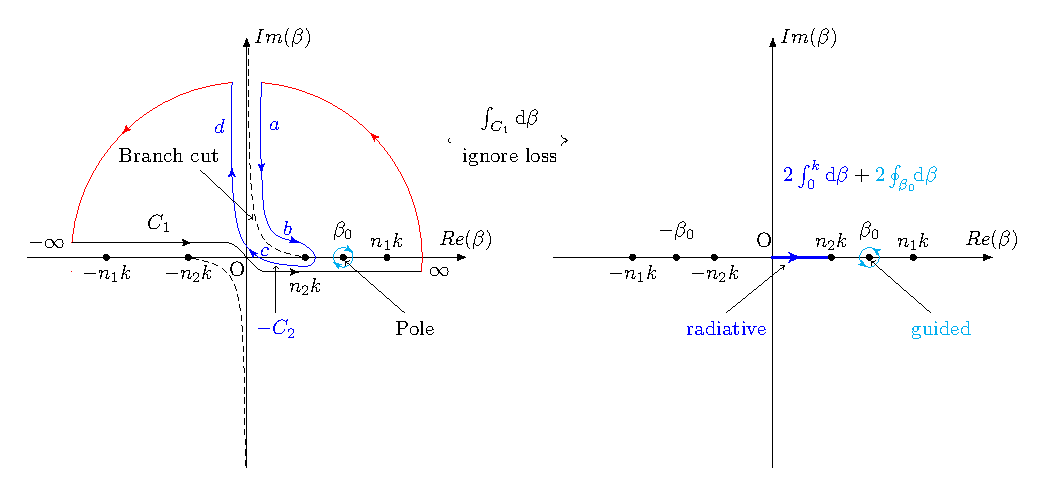
\includegraphics[scale=0.75]{../media/Figs/contourplot_upper}}
\end{minipage}
\par\medskip
\begin{minipage}{.91\linewidth}
\centering
\subfloat[]{\label{contourplot_lower}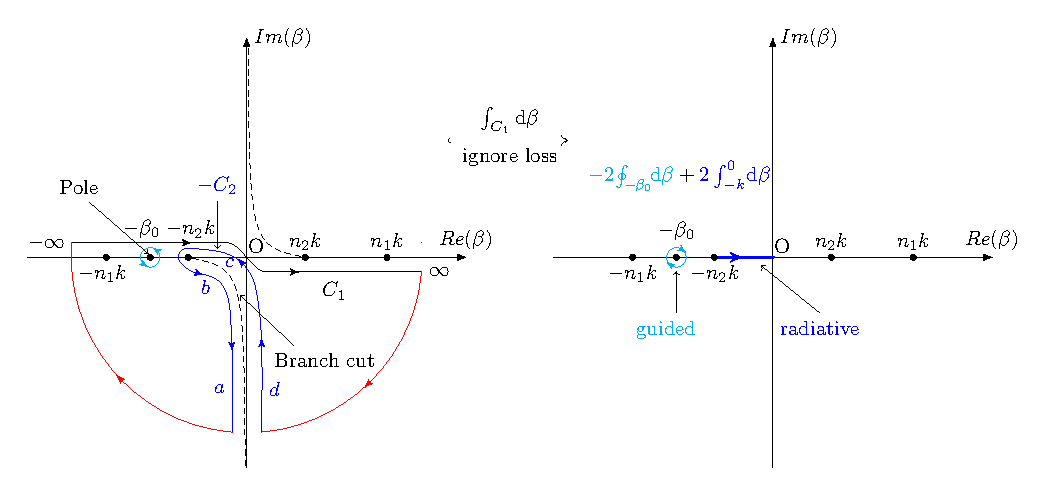
\includegraphics[scale=0.75]{../media/Figs/contourplot_lower}}
\end{minipage}
\caption[Contour integrations to decompose the guided and radiation modes of a dipole radiation problem in presence of a single mode waveguide.]{Integration paths. For the case that $ z>0 $, we can use the zero-valued contour integral path drawn in subfig.~\ref{contourplot_upper} to calculate the integration along path $ C_1 $. The simplified integration path by ignoring waveguide losses is given on the right-hand-side. It only contains the forward propagating mode contributions with radiation and guided mode components as divided through the real axis integral and the loop-hole integral. For the $ z<0 $ case, the contour integral analysis is given in subfig.~\ref{contourplot_lower}, which only includes the backward propagating mode contributions.}
\label{fig:integralpath}
\end{figure}

Now, we only consider the $ m=\pm 1 $ modes, and hence Equs.~\ref{ET0Rexpand}, ~\ref{BT0Rexpand} and the corresponding $ \phi $ and $ r\!_\perp $ components can be explicitly expressed as contour integrals as below
\begin{subequations}\label{ET0RC1}
\begin{align}
\mathcal{E}^{(T)}_z &= \sum_{m=\pm 1} \int_{C_1} \mathrm{d}\beta e^{im(\phi-\phi') + i\beta (z-z')} c_{m\beta} J_m (hr\!_\perp),\\
% + B_{m\beta} Y_m(hr\!_\perp)\right],\\
\mathcal{E}^{(0)}_{z} &= \sum_{m=\pm 1} \int_{C_1} \mathrm{d}\beta e^{im(\phi-\phi') + i\beta (z-z')} \mathcal{E}^{(0)}_{z,m\beta}(r\!_\perp)\\
\mathcal{E}^{(R)}_z &= \sum_{m=\pm 1} \int_{C_1} \mathrm{d}\beta e^{im(\phi-\phi') + i\beta (z-z')} a_{m\beta} H_m^{(1)} (pr\!_\perp),
\end{align}
\end{subequations}
\begin{subequations}\label{BT0RC1}
\begin{align}
\mathcal{B}^{(T)}_z &= \sum_{m=\pm 1} \int_{C_1} \mathrm{d}\beta e^{im(\phi-\phi') + i\beta (z-z')} d_{m\beta} J_m (hr\!_\perp),\\
% + E_{m\beta} Y_m(hr\!_\perp)\right],\\
\mathcal{B}^{(0)}_{z} &= \sum_{m=\pm 1} \int_{C_1} \mathrm{d}\beta e^{im(\phi-\phi') + i\beta (z-z')} \mathcal{B}^{(0)}_{z,m\beta}(r\!_\perp)\\
\mathcal{B}^{(R)}_z &= \sum_{m=\pm 1} \int_{C_1} \mathrm{d}\beta e^{im(\phi-\phi') + i\beta (z-z')} b_{m\beta} H_m^{(1)} (pr\!_\perp).
\end{align}
\end{subequations}
To distinguish the bound and radiation modes contributions, one can use the integral path along $ C_1 $ (see Fig.(\ref{fig:integralpath})) and find the equivalent integral path detouring the branch cuts and isolated poles which will be discussed next. 

For the free-dipole radiation components, the $ C_1 $ integral path is almost the real integral path from $ -\infty $ to the $ +\infty $ except for the branch point at $ \pm k $. The sign of $ \beta $ indicates the propagation direction of the field. The free-dipole components only yield the radiation mode contributions to the total Green's dyadic. This is because the dipole radiation only occurs outside of the fiber, and always in the radiation potential zone using the equivalent scattering potential model. 

For the reflection and transmission components of the field, there are poles in the $ a_{m\beta} $, $ b_{m\beta} $, $ c_{m\beta} $ and $ d_{m\beta} $ coefficients. There are also branch cuts hidden in the Bessel and Hankel function components of their expressions. Depending on the sign of $ (z-z') $, the integral paths and their simplification are shown in Fig.(\ref{fig:integralpath}). The bound modes are associated with poles, and hence can be represented as residues if asymptotic approximation can be made. Therefore, the guided mode contribution part of the reflection and transmission components can be given by
\begin{subequations}\label{ET0RRes}
\begin{align}
\mathcal{E}^{(T)}_z &= \sum_{m=\pm 1} \oint_{\beta_{1,m}}  e^{im(\phi\!-\!\phi') + i\beta (z\!-\!z')} c_{m\beta} J_m (hr\!_\perp),\\
%\mathcal{E}^{(0)}_{z} &= 2\pi i \sum_{m=\pm 1} \sum_{\beta_{1,m=\pm 1}}\mathrm{Res}\left[  e^{im(\phi-\phi') + i\beta (z-z')} \mathcal{E}^{(0)}_{z,m\beta}(r\!_\perp)\right]_{\beta=\beta_{1,m}},\\
\mathcal{E}^{(R)}_z &= \sum_{m=\pm 1} \oint_{\beta_{1,m}} e^{im(\phi\!-\!\phi') + i\beta (z\!-\!z')} a_{m\beta} H_m^{(1)} (pr\!_\perp),
\end{align}
\end{subequations}
\begin{subequations}\label{BT0RRes}
\begin{align}
\mathcal{B}^{(T)}_z &= \sum_{m=\pm 1} \oint_{\beta_{1,m}} e^{im(\phi\!-\!\phi') + i\beta (z\!-\!z')} d_{m\beta} J_m (hr\!_\perp),\\
%\mathcal{B}^{(0)}_{z} &= 2\pi i \sum_{m=\pm 1} \sum_{\beta_{1,m=\pm 1}}\mathrm{Res}\left[  e^{im(\phi-\phi') + i\beta (z-z')} \mathcal{B}^{(0)}_{z,m\beta}(r\!_\perp)\right]_{\beta=\beta_{1,m}}, \\
\mathcal{B}^{(R)}_z &= \sum_{m=\pm 1} \oint_{\beta_{1,m}} e^{im(\phi\!-\!\phi') + i\beta (z\!-\!z')} b_{m\beta} H_m^{(1)} (pr\!_\perp).
\end{align}
\end{subequations}
%\begin{subequations}\label{ET0RRes}
%\begin{align}
%\mathcal{E}^{(T)}_z &= 2\pi i \sum_{m=\pm 1} \sum_{\beta_{1,m=\pm 1}}\mathrm{Res}\left[  e^{im(\phi\!-\!\phi') + i\beta (z\!-\!z')} c_{m\beta} J_m (hr\!_\perp)\right]_{\beta=\beta_{1,m}},\\
%% + B_{m\beta} Y_m(hr\!_\perp)\right],\\
%\mathcal{E}^{(0)}_{z} &= 2\pi i \sum_{m=\pm 1} \sum_{\beta_{1,m=\pm 1}}\mathrm{Res}\left[  e^{im(\phi-\phi') + i\beta (z-z')} \mathcal{E}^{(0)}_{z,m\beta}(r\!_\perp)\right]_{\beta=\beta_{1,m}},\\
%\mathcal{E}^{(R)}_z &= 2\pi i \sum_{m=\pm 1} \sum_{\beta_{1,m=\pm 1}}\mathrm{Res}\left[ e^{im(\phi\!-\!\phi') + i\beta (z\!-\!z')} a_{m\beta} H_m^{(1)} (pr\!_\perp)\right]_{\beta=\beta_{1,m}},
%\end{align}
%\end{subequations}
%\begin{subequations}\label{BT0RRes}
%\begin{align}
%\mathcal{B}^{(T)}_z &= 2\pi i \sum_{m=\pm 1} \sum_{\beta_{1,m=\pm 1}}\mathrm{Res}\left[ e^{im(\phi\!-\!\phi') + i\beta (z\!-\!z')} d_{m\beta} J_m (hr\!_\perp)\right]_{\beta=\beta_{1,m}},\\
%% + E_{m\beta} Y_m(hr\!_\perp)\right],\\
%\mathcal{B}^{(0)}_{z} &= 2\pi i \sum_{m=\pm 1} \sum_{\beta_{1,m=\pm 1}}\mathrm{Res}\left[  e^{im(\phi-\phi') + i\beta (z-z')} \mathcal{B}^{(0)}_{z,m\beta}(r\!_\perp)\right]_{\beta=\beta_{1,m}}, \\
%\mathcal{B}^{(R)}_z &= 2\pi i \sum_{m=\pm 1} \sum_{\beta_{1,m=\pm 1}}\mathrm{Res}\left[ e^{im(\phi\!-\!\phi') + i\beta (z\!-\!z')} b_{m\beta} H_m^{(1)} (pr\!_\perp)\right]_{\beta=\beta_{1,m}}.
%\end{align}
%\end{subequations}

The radiation mode contributions of the reflection and transmission components are associated with the branch cuts $ C_2 $~\cite{Klimov2004} in Fig.(\ref{fig:integralpath}).
\begin{subequations}\label{ET0RC2}
\begin{align}
\mathcal{E}^{(T)}_z &= \sum_{m=\pm 1} \int_{C_2} \mathrm{d}\beta e^{im(\phi-\phi') + i\beta (z-z')} c_{m\beta} J_m (hr\!_\perp)\\
&\approx \sum_{m=\pm 1} 2\int_{-n_2k}^{n_2k} \mathrm{d}\beta e^{im(\phi-\phi') + i\beta (z-z')} c_{m\beta} J_m (hr\!_\perp),\\
%\mathcal{E}^{(0)}_{z} &= \sum_{m=\pm 1} \oint_{C_2} \mathrm{d}\beta e^{im(\phi-\phi') + i\beta (z-z')} \mathcal{E}^{(0)}_{z,m\beta}(r\!_\perp),\\
\mathcal{E}^{(R)}_z &= \sum_{m=\pm 1} \oint_{C_2} \mathrm{d}\beta e^{im(\phi-\phi') + i\beta (z-z')} a_{m\beta} H_m^{(1)} (pr\!_\perp)\\
&\approx \sum_{m=\pm 1} 2\int_{-n_2k}^{n_2k} \mathrm{d}\beta e^{im(\phi-\phi') + i\beta (z-z')} a_{m\beta} H_m^{(1)} (pr\!_\perp),
\end{align}
\end{subequations}
\begin{subequations}\label{BT0RC2}
\begin{align}
\mathcal{B}^{(T)}_z &= \sum_{m=\pm 1} \oint_{C_2} \mathrm{d}\beta e^{im(\phi-\phi') + i\beta (z-z')} d_{m\beta} J_m (hr\!_\perp)\\
&\approx \sum_{m=\pm 1} 2\int_{-n_2k}^{n_2k} \mathrm{d}\beta e^{im(\phi-\phi') + i\beta (z-z')} d_{m\beta} J_m (hr\!_\perp),\\
%\mathcal{B}^{(0)}_{z} &= \sum_{m=\pm 1} \oint_{C_2} \mathrm{d}\beta e^{im(\phi-\phi') + i\beta (z-z')} \mathcal{B}^{(0)}_{z,m\beta}(r\!_\perp),\\
\mathcal{B}^{(R)}_z &= \sum_{m=\pm 1} \oint_{C_2} \mathrm{d}\beta e^{im(\phi-\phi') + i\beta (z-z')} b_{m\beta} H_m^{(1)} (pr\!_\perp)\\
&\approx \sum_{m=\pm 1} 2\int_{-n_2k}^{n_2k} \mathrm{d}\beta e^{im(\phi-\phi') + i\beta (z-z')} b_{m\beta} H_m^{(1)} (pr\!_\perp).
\end{align}
\end{subequations}
Above, the approximation works when the waveguide is lossless and hence the branch lines along the imaginary axis of the $ \beta $ plane can be ignored. The factor of $ 2 $ comes from the sign flip of the two branch lines parallel to the real axis in the $ \beta $ plane ($ 2=1-\mathrm{e}^{\pi i} $), and physically corresponds to the degeneracy of $ 2 $ degrees of freedom of the polarization of the radiation modes in the transverse plane. Although we use the integral limit from $ -n_2k $ to $ n_2k $, the integral limit, in practice, should be either $ 0 \rightarrow n_2k$ or $ -n_2k\rightarrow 0 $ depending on the propagation directions we are interested in. 

One can obtain the bound and radiation field components with the dipole oriented in $ z $, $ \phi $ and $ r\!_\perp $ directions by substituting the $ \bmc{E}^{(0)}_{m\beta}(r\!_\perp) $ expressions for corresponding cases into Equs.~\ref{ET0RRes},~\ref{BT0RRes},~\ref{ET0RC2} and~\ref{BT0RC2}. 

To calculate the bound modes, we need to calculate the residues at isolated poles with $ \beta_{1,m} $ and $ m=\pm 1 $. The poles can be found by using the condition that
\begin{align}
D=P^2+QR=0,
\end{align}
or
\begin{align}\label{pole4beta}
&\beta^2m^2k^4\left(J_m(ha) H_m^{(1)}(pa) \right)^2 (\varepsilon_f-1)^2\nonumber\\
-& h^2p^2a^2k^2 \left(hJ_m(ha) \dd{}{(pa)}H_m^{(1)}(pa)-pH_m^{(1)}(pa)\dd{}{(ha)}J_m(ha) \right)\nonumber\\ &\left(hJ_m(ha) \dd{}{(pa)}H_m^{(1)}(pa)-\varepsilon_f pH_m^{(1)}(pa)\dd{}{(ha)}J_m(ha) \right)=0.
\end{align}
Here are some useful relationships to solve the equation above:
\begin{align}
J_{-m}(z)=(-1)^nJ_n(z),\, &\quad H_{-m}^{(1)}(z)=e^{m\pi i}H_m^{(1)}(z),\\
\dd{}{z}J_m(z) &= \frac{1}{2} \left( J_{m-1}(z)-J_{m+1}(z) \right),\\ 
\dd{}{z}H^{(1)}_m(z) &= \frac{1}{2} \left( H^{(1)}_{m-1}(z)-H^{(1)}_{m+1}(z) \right).
\end{align}
We can rewrite Eq.~\ref{pole4beta} as
\begin{align}\label{pole4beta2}
&\beta^2m^2k^2\left(J_m\!(ha) H_m^{(\!1\!)}\!(pa) \right)^2 (\varepsilon_f-1)^2\nonumber\\
=& \frac{h^2p^2a^2}{4} \left[hJ_m\!(ha)\! \left( H^{(\!1\!)}_{m-1}\!(pa)\!-\! H^{(\!1\!)}_{m+1}\!(pa) \right)\!-\! pH_m^{(\!1\!)}\!(pa)\left( J_{m-1}\!(ha)\!-\! J_{m+1}\!(ha) \right) \right]\nonumber\\ 
&\left[hJ_m\!(ha) \left( H^{(\!1\!)}_{m-1}\!(pa)\!-\! H^{(\!1\!)}_{m+1}\!(pa) \right)\!-\! \varepsilon_f pH_m^{(\!1\!)}\!(pa)\left( J_{m-1}\!(ha)\!-\! J_{m+1}\!(ha) \right) \right].
\end{align}
Since both $ h $ and $ p $ are functions of $ \beta $, the equation above is complicated for solving $ \beta $. If $ ka<0.8 $, asymptotic approximation is good enough to solve Eq.~\ref{pole4beta2} and give an analytical solution for $ \beta $~\cite{Klimov2004}. However, in our nanofiber case, the $ ka<0.8 $ condition is not satisfied. We should be able to numerically solve Eq.~\ref{pole4beta2} for $ \beta $ as the characteristic constant for the guided mode with $ m=\pm 1 $. \textcolor{red}{Q: we should prove Eq.~\eqref{pole4beta2} is equivalent to the eigen equation of $ \beta $ for the bare fiber case. Useful relationship: $ K_n(x)=\frac{\pi}{2}i^{n+1}H_n^{(1)}(ix) $.}

Numerically, the eigenwavevector $ \beta_0 $ is indistinguishable with the intrinsic nanofiber eigen mode wavevector, in the regime we are interested in.

Next, we can solve the bound modes by differentiating the functions inside of $ Res $ signs and inserting the values of $ \beta_{1,m=\pm 1} $. %\textcolor{red}{(Q: are those poles all of order 1?)} 
The transverse components of the fields can be obtained from the longitudinal components using the relations of Eq.~\ref{EHzgauss}. 
%Sample numerical calculations has been performed, and results are documented in the NanofiberProjectPlots.pdf (Dropbox folder, \url{Nanofiber/Code/Matlab/Plots}). The primary plots show that there are phase shifts for the transmitted and reflected lights so that the mode profile is not symmetric to the $ x $ axis where the atom lies on; the reflected light field has a backaction on the atom tending to move it off the trapping point; the $ m=\pm 1 $ modes are not balanced... 
Our derivation results had be checked by reproducing the decay rates following Klimov's paper~\cite{Klimov2004}. 

To calculate the total decay rate of the atom with the enhancement due to the radiation, we need to find out the functions describing the branch cuts and the integration path for the radiation modes. The equation defining the branch cut is given by
\begin{align}\label{branchcutequ}
\mathrm{Im}\left[p \right] &=0\\
\mathrm{Im}\left[h\right] &=0.
\end{align}
By setting $ \beta=x+iy $, we can rewrite the first equation above as
\begin{align}
p&=\sqrt{k^2-\beta^2}\\
&=\left[(k^2-x^2+y^2)^2 + 4x^2y^2 \right]^{1/4}e^{\frac{i}{2}\arctan\frac{-2xy}{k^2-x^2+y^2}}.
\end{align}
Hence Eq.~\ref{branchcutequ} yields
\begin{align}
0&= \left[(k^2-x^2+y^2)^2 + 4x^2y^2 \right]^{1/4} \sin \left[\frac{1}{2}\arctan\frac{-2xy}{k^2-x^2+y^2} \right]\\
&= \frac{1}{\sqrt{2}} \left[(k^2\!-\! x^2\!+\! y^2)^2 \!+\! 4x^2y^2 \right]^{1/4} \sqrt{1\!-\!\cos \left(\arctan\frac{-2xy}{k^2\!-\! x^2\!+\! y^2} \right)}\\
&= \frac{1}{\sqrt{2}} \left[(k^2\!-\!x^2\!+\! y^2)^2 \!+\! 4x^2y^2 \right]^{1/4} \sqrt{1\!-\! \frac{k^2\!-\! x^2\!+\! y^2}{\left[(k^2\!-\! x^2\!+\! y^2)^2 \!+\! 4x^2y^2 \right]^{1/2}} }\\
&=\sqrt{\left[(k^2-x^2+y^2)^2 + 4x^2y^2 \right]^{1/2}-(k^2-x^2+y^2)},
\end{align}
which gives
\begin{align}
\left[(k^2-x^2+y^2)^2 + 4x^2y^2 \right]^{1/2}&=(k^2-x^2+y^2),\\
\Leftrightarrow \qquad \qquad \qquad \qquad \qquad x^2y^2&=0.\label{branchcut2}
\end{align}
Obviously, the $ x $ axis between $ [-k,k] $ and the entire $ y $ axis are the branch cuts. To separate the branches into upper and lower parts, we can define an arbitrary small positive number $ \delta\epsilon\rightarrow 0 $ so that Eq.~\ref{branchcut2} gives
\begin{align}
xy&=\delta\epsilon.
\end{align}
Similarly, the condition for $ \mathrm{Im}[h]=0 $ gives the same result. To make the field components homomorphic at any point in the complex $ \beta $ plane, we choose the branch cuts that satisfy 
\begin{align}
xy&>\delta\epsilon>0.
\end{align}
Calling the physics meaning of radiation mode, we also have 
\begin{align}
-n_2k<x<n_2k.
\end{align}
In this way, the branch cuts as a hyperbola-type lines are symmetrically separated into top-right and lower-left parts, and are very close to the $ x- $ and $ y- $axes. For the top-right branch, one can choose the integration path as shown in Fig.~\ref{fig:integralpath} to apply the contour integral detouring the branch cut. 

%\scalefig{Figs/contourpath2}{0.8}{Integration path of the contour integral for radiation modes.}

In the case that the nanofiber can be treated as a lossless medium, the contour integral can be treated as an integral over real axis from $ -kn_2 $ to $ kn_2 $. 
We illustrate the division of the guided and unguided mode contributions to the integration over $ \beta $ in Fig.~\ref{fig:integralpaths} and how the contour integrals in different regions to be calculated. 

\begin{figure}[!tbp]
\centering\makebox[\textwidth]{
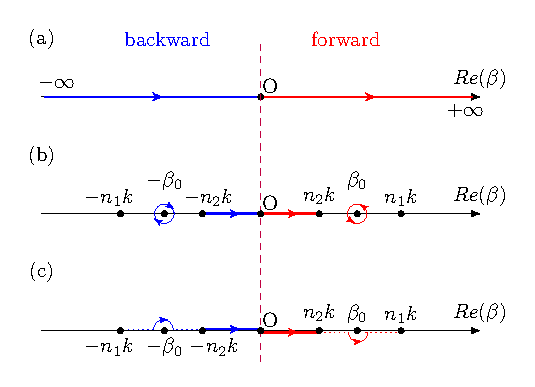
\includegraphics[width=0.85\textwidth]{../media/Figs/integratepath_GF}}
\caption[Integral paths for the dyadic Green's function calculations when loss is negligible.]{Integral paths for the dyadic Green's function calculations. Part (a) is the integral path for the dipole's free-space field contribution calculation [see, for example, Eq.~\eqref{ET0RC1}]. Part (b) is the integral path for the reflected and transmitted field contributions calculation [see, for example, Eq.~\eqref{ET0RC1}]. Part (c) is the integral path for the dyadic Green's function calculation using the eigenmode decomposition method [see Eqs.~\eqref{Eq::GreensEigenmodes} and~\eqref{Eq::GreensunguidedEigenmodes}]. The integral paths on the left-hand-side (in blue) indicate the backward propagating contributions, while the right-hand-side (in red) parts corresponding to the forward propagating contributions. For the eigenmode decomposition method in part (c), if one choose to use $ f=\pm 1 $ to indicate the propagation direction, then only the $ \beta>0 $ portion of integral path will be applied. }
\label{fig:integralpaths}
\end{figure}

As shown in section~\ref{sec:eigenmodesofwaveguides}, the guided and radiation modes contribution to the dyadic Green's function can be identified through the specific choice of integral paths. In Fig.~\ref{fig:integralpaths}, part (a) shows the integral path to calculate the dipole free-space contribution which does not yield guided mode contribution to the total dyadic Green's function. Part (b) of the figure shows the loop and real-valued integral paths of the guided and radiation mode divisions to the reflected and transmitted field components. The $ \mathrm{Re}(\beta)<0 $ and $ \mathrm{Re}(\beta)>0 $ parts correspond to the backward and forward propagating contributions, respectively. Part (c) of the figure indicates the integral path using the eigenmode decomposition method in the case that the sign of $ \mathrm{Re}(\beta) $ indicates the propagation directions. Depending on the propagation directions, we should choose the right integral paths for the corresponding methods adopted, and different methods should yield the same result. 


With all of the field components solved given a dipole vector, the dyadic Green's function can be calculated with three parts: the part due to free-dipole radiation, $ \GFT_0(\br,\br') $, the field reflection part due to the presence of the waveguide interface, $ \GFT_R(\br,\br') $, and the part due to mode transmission through the waveguide, $ \GFT_T(\br,\br') $. The former two parts generate the unguided mode contribution to the total dyadic Green's function, and the third part forms the guided mode contribution to the total dyadic Green's function. The $ ij $th components of the three parts of the dyadic Green's function can then be calculated by (see Eq.~\eqref{eq:GFTijEd})
\begin{align}
G_0^{ij}(\br,\br') &= \frac{\mathcal{E}_i^{(0)}(\br)}{d_j(\br')},\\
G_R^{ij}(\br,\br') &= \frac{\mathcal{E}_i^{(R)}(\br)}{d_j(\br')},\\
G_T^{ij}(\br,\br') &= \frac{\mathcal{E}_i^{(T)}(\br)}{d_j(\br')},
\end{align}
where $ \mathcal{E}_i^{(A)}\,(A=0,R,T) $ are the $ i $th free-dipole radiation, interface reflection and mode transmission electric component due to the corresponding dipole $ d_j $ orientated along the $ \mathbf{e}_j $ direction. The total dyadic Green's function 
\begin{align}
\GFT(\br,\br')=\GFT_0(\br,\br')+\GFT_R(\br,\br')+\GFT_T(\br,\br') .
\end{align} 


%</nanofiberradiationproblem>


%<*choozingSWGs>
\chapter{The choice of square waveguides for this study}\label{chap:choozingSWGs}
\section{Phase walkoff problems of rectangular waveguides}
Based on the enhanced QND-measurement--induced spin squeezing protocol we have studied in Ref.~\cite{Qi2017Enhanced}, a key to generate a strong spin squeezing effect (for precise measurement or generating non-classical collective states) is to allow the mode transformation between the ``local oscilator" mode and the ``signal mode". We can them as the $ H $ mode and $ V $ mode. In general, the field operator for the QND measurement can be written as 
\begin{align}\label{eq:EdifferentHV}
\hat{\mathbf{E}}^{(+)}(r\!_\perp,\phi,z;t) &= \sqrt{ \frac{2 \pi \hbar \omega_0}{ v_g^H} } \mathbf{u}_H(r\!_\perp,\phi) \hat{a}_H(z,t)  e^{i (\beta_0^H z- \omega_0 t)}\nn\\
&\quad +\sqrt{ \frac{2 \pi \hbar \omega_0}{ v_g^V} } \mathbf{u}_V(r\!_\perp,\phi) \hat{a}_V(z,t)  e^{i (\beta_0^V z- \omega_0 t)},
\end{align}
where $ v_g^{H/V} $ and $ \beta_0^{H/V} $ are the group velocities and propagation constants of the $ H $ and $ V $ modes, respectively. When a rectangular waveguide is used, $ v_g^H $ and $ v_g^V $, so as the projected mode constants $ \beta_0^H $ and $ \beta_0^V $, become different or non-degenerate.
The offset of $ v_g^{H/V} $ and $ \beta_0^{H/V} $ for the two guided modes could lead to a walkoff effect of the modes and cause an intrinsic phase shift.
We want to avoid this walkoff effect, unless the phase shift between the two modes at atom positions are multiples of $ 2\pi $, which is hard to implement as we will show next, which is mostly my conversion with other collaborators on writing Ref.~\cite{Qi2017Enhanced}.

\section{Optimal width of a \SWG to tolerate fabrication imperfections}

I made four plots when I and Dr. Jongmin Lee were working on determining the
preferable dimension of the waveguides. See Fig.~\ref{fig:ng_rect_dwg}.

\begin{figure}[!tbp]
\centering
\begin{minipage}[h]{\linewidth}
 %\begin{tabular}{*{2}{b{0.2\textwidth-2\tabcolsep}}}
  \subfloat[h][]{
    %% This file was created by matlab2tikz.
%
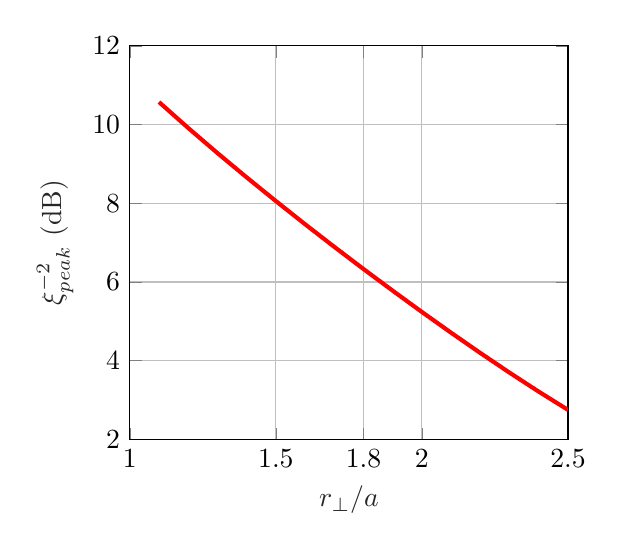
\begin{tikzpicture}

\begin{axis}[%
width=5.565cm,
height=5cm,
at={(0cm,0cm)},
scale only axis,
xmin=1.0000,
xmax=2.5000,
xtick={1.0000,1.5000,1.8000,2.0000,2.5000},
xlabel style={font=\color{white!15!black}},
xlabel={$r_\perp/a$},
ymin=2.0000,
ymax=12.0000,
ylabel style={font=\color{white!15!black}},
ylabel={$\xi^{-2}_{peak}$ (dB)},
axis background/.style={fill=white},
xmajorgrids,
ymajorgrids
]
\addplot [color=red, line width=1.5pt, forget plot]
  table[row sep=crcr]{%
1.1000	10.5712\\
1.2000	9.9128\\
1.3000	9.2762\\
1.4000	8.6588\\
1.5000	8.0571\\
1.6000	7.4685\\
1.7000	6.8935\\
1.8000	6.3307\\
1.9000	5.7799\\
2.0000	5.2394\\
2.1000	4.7118\\
2.2000	4.1974\\
2.3000	3.6980\\
2.4000	3.2157\\
2.5000	2.7531\\
};
\end{axis}
\end{tikzpicture}%
    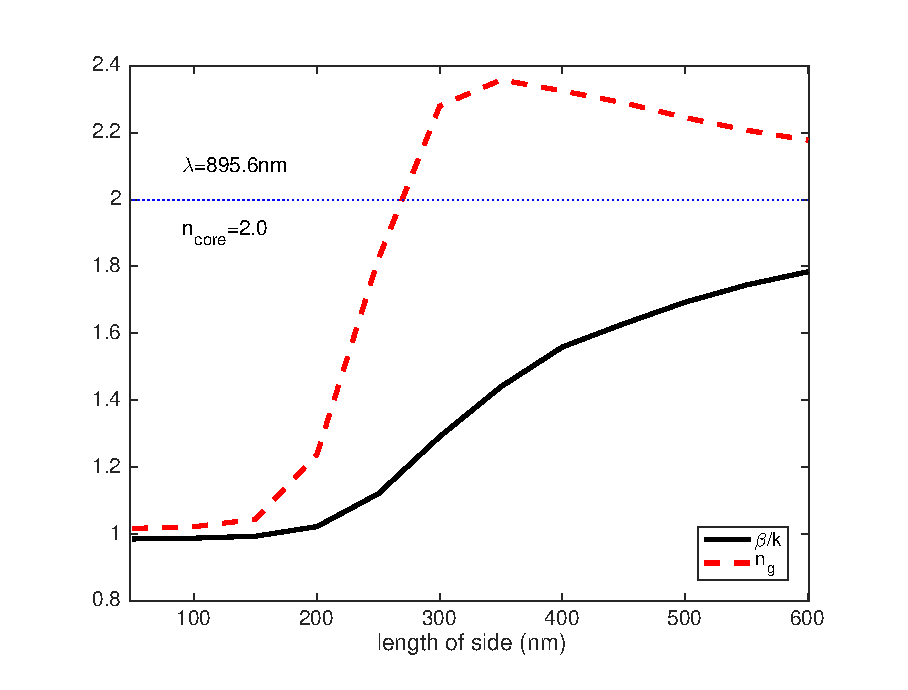
\includegraphics[width=0.48\linewidth]{../media/Figs/ng_D1_dwg}
    \label{fig:ng_D1_dwg}
    }
    \hfill
  \subfloat[h][]{
      \label{fig:ng_D2_dwg}
      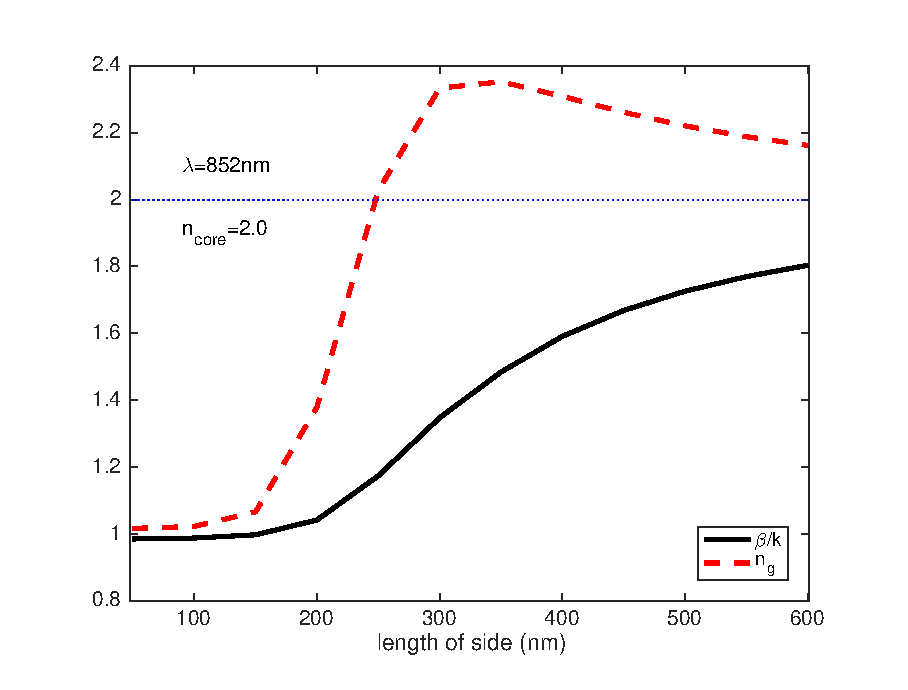
\includegraphics[width=0.48\linewidth]{../media/Figs/ng_D2_dwg}
      %% This file was created by matlab2tikz.
%
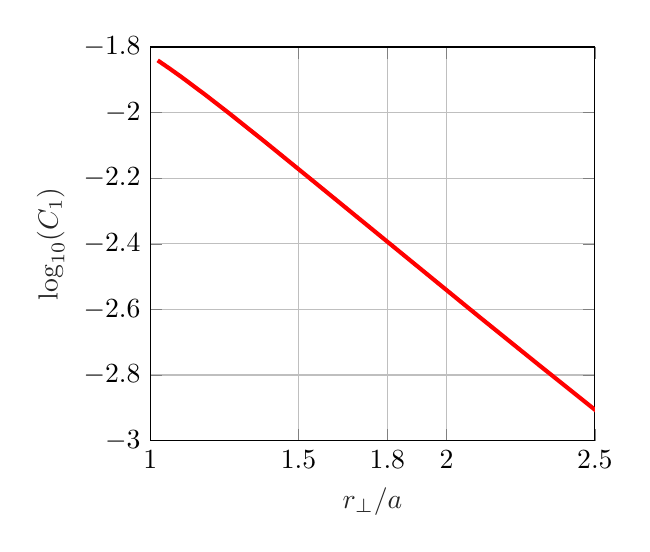
\begin{tikzpicture}

\begin{axis}[%
width=5.647cm,
height=5cm,
at={(0cm,0cm)},
scale only axis,
xmin=1.0000,
xmax=2.5000,
xtick={1.0000,1.5000,1.8000,2.0000,2.5000},
xlabel style={font=\color{white!15!black}},
xlabel={$r_\perp/a$},
ymin=-3.0000,
ymax=-1.8000,
ylabel style={font=\color{white!15!black}},
ylabel={$\log_{10}(C_1)$},
axis background/.style={fill=white},
xmajorgrids,
ymajorgrids
]
\addplot [color=red, line width=1.5pt, forget plot]
  table[row sep=crcr]{%
1.0251	-1.8409\\
1.0653	-1.8658\\
1.1055	-1.8917\\
1.1859	-1.9459\\
1.2663	-2.0022\\
1.3869	-2.0891\\
1.5477	-2.2073\\
2.1106	-2.6230\\
2.3116	-2.7696\\
2.5126	-2.9148\\
};
\end{axis}
\end{tikzpicture}%
      }
   \end{minipage}\vfill
   \begin{minipage}[h]{\linewidth}
    %\begin{tabular}{*{2}{b{0.2\textwidth-2\tabcolsep}}}
     \subfloat[h][]{
       %\input{fig/square waveguide_peakxi_rp_NA2500.tex}
       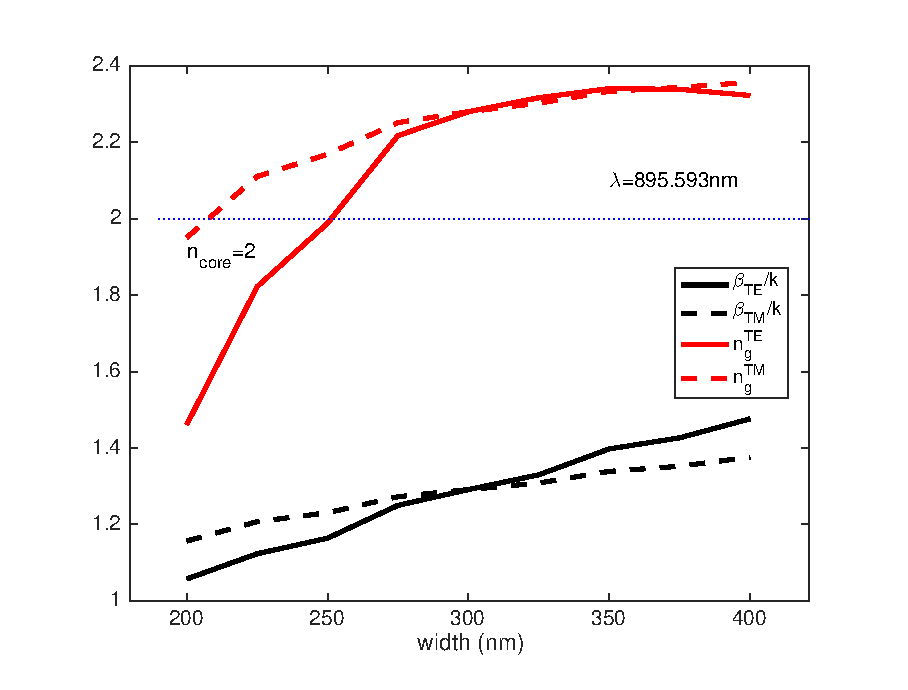
\includegraphics[width=0.48\linewidth]{../media/Figs/ng_D1_rectwg_dwg}
       \label{fig:ng_D1_rectwg_dwg}
       }
       \hfill
     \subfloat[h][]{
         \label{fig:ng_D2_rectwg_dwg}
         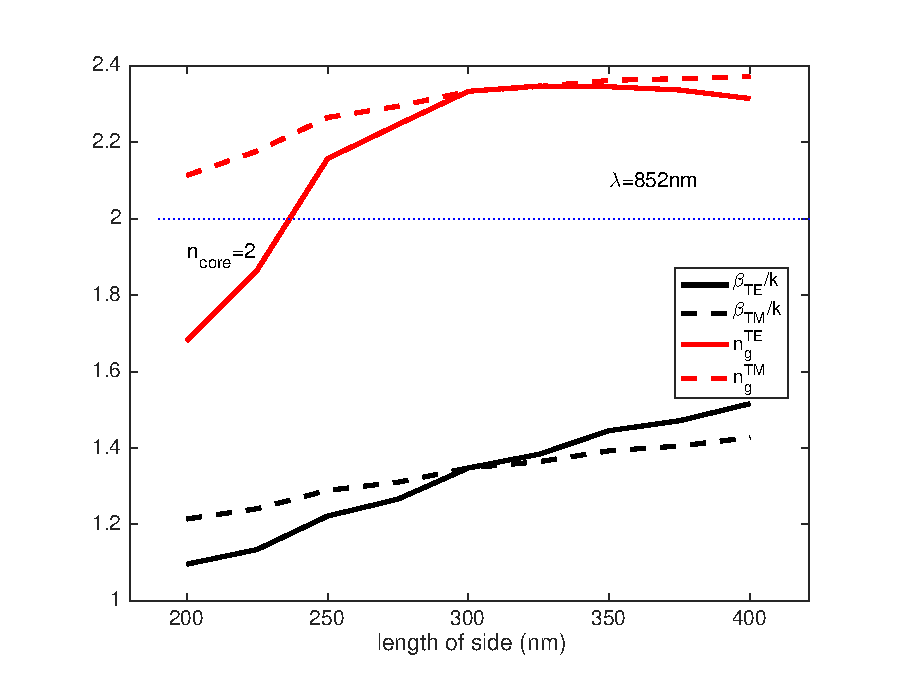
\includegraphics[width=0.48\linewidth]{../media/Figs/ng_D2_rectwg_dwg}
         %\input{fig/square waveguide_C1_y.tex}
         }
   \end{minipage}
\caption[Optimal choice of waveguide width to tolerate fabrication imperfections.]{Group index of refraction with changing width of a square waveguide ($ n_1=2.0,\,w=300 $ nm) at cesium's D1 line (a) and D2 line (b). Group indices of refraction and the phase indices of refraction for the fundamental quasi-\TE and quasi-\TM modes of an imperfect \SWG with a side changing its length ($ x $ axis) at the D1 line (c) and the D2 line (d).}\label{fig:ng_rect_dwg}
\end{figure}

In the figure, (a) and (b) show that the group index of refraction ng reaches the
peak value at $\sim 300$ nm for both D1 line (a) and D2 line (b). That plateaus
at the $300$ nm $x$-axis value of the $n_g$ curves as a function
of the width of a square waveguide imply that $n_g$ will be the most
robust case in presence of fabrication fluctuations. 1\% of fabrication
imperfection may not be a big issue to worry about in our case.

In figure (c) and (d), I fix one side of the waveguide to be $300$ nm while
varying the other side from $200$ nm to $400$ nm, and plot out the phase index
of refraction ($beta/k$) and the group index of fraction ($n_g$) for the
non-degenerate fundamental quasi-\TE and quasi-\TM modes. Of course, our formulas of
effective mode areas for spin squeezing should be modified for the
non-degenerate mode case. I didn't do the detailed calculation, but I'd
think the modification is the following: the $n_g$ in the formula of the effective interaction mode area for our Faraday spin squeezing protocol~\cite{Qi2017Enhanced}, $A_{\rm Far}$, should be replaced with the geometric average of $n_g^{TE}$ and $n_g^{TM}$, that is $\sqrt{n_g^{V} \times n_g^{H}}$ when $V$ and $H$ modes are the quasi-\TE and quasi-\TM modes; the equation for the  input mode area, $A_0$, maintains its original form. In the end,
the cooperavity formula should be modified by a factor of the square
root of the ratio between $n_g^V$ and $n_g^H$, where the input probe is
polarized along the $H$ direction and atoms are trapped on the $V$ axis.
From the plots of (c) and (d) at D1 and D2 lines, you see that the
phase indices of refraction are only barely distinguishable between the two modes with
$10\%/k$ maximum when one side of the waveguide is $200$ nm in the plots. The phase
matching condition basically tells us that the two groups of atoms
should be trapped in a minimum distance of $10\times k$, which might be too long to implement considering the great photon loss through the waveguide. Notice that the phase
difference between the two modes scales almost linearly when one side of
the waveguide decreases.

On the other hand, the ratio between the two group indices increases
dramatically when one side of the waveguide is shortened. But when we
plug in the numbers, with a $200$ nm $\times$ $300$ nm waveguide, the enhancement of
cooperativity is only about $15\%$ from the $300$ nm $\times$ $300$ nm square waveguide
case. Considering the trapping potential well gets sharper when the
corresponding side of the waveguide decreases, I think the most
important benefit of using a rectangular waveguide might be the ability
to make the trapping potential sharp on the direction parallel to the
nearest side of the waveguide. I haven't considered the quantized
trapping potential level splitting on the vertical direction, but I feel
it's also good for the experiment.

For the phase mismatch issue, I think as along as the group velocities
do not make the light pulses of the two modes walk off too much in the
waveguide range, the measurement signal as the time integral under a
resolution of ns or even longer won't tell the difference between the
signals from the two groups of atoms. Since the birefringence rotation due to the mode distortion 
is deterministic given the number of atoms, we might be able to
compensate that phase drafting and extract the pure Faraday rotation
measurement signal in the end.

%</choozingSWGs>

%###################################################################################
\bibliographystyle{../styles/abbrv-alpha-letters-links}
\bibliography{../refs/Archive}
%%%%%%%%%%%%%%%%%%%%%%%%%%%%%%%%%%%%%%%%%%%%%%%%%%%%%%%%%%%%%%%%%%%%%%%%%%%%%%%%%%%%

\printindex
\end{document}
